\documentclass[sigconf,nonacm]{acmart}

\usepackage{enumitem}
\setlist[enumerate,1]{label=\arabic*.}
\usepackage{siunitx}
\usepackage{hyperref}  % optional, for clickable links
\usepackage{cleveref}  % always load *after* hyperref
\usepackage{graphicx}
\usepackage{tabularx}
\usepackage{float}
\usepackage[table]{xcolor}


\AtBeginDocument{%
  \providecommand\BibTeX{{%
    Bib\TeX}}}

\settopmatter{printfolios=true}

\begin{document}
\title{Assignment 2 Report: Wi-Fi Analysis}
\author{Yusuf Erdem Nacar}
\affiliation{%
  \institution{Technische Universit{\"a}t M{\"u}nchen \\ TUM Chair for Connected Mobility \\ Connected Mobility Basics - SS25}
  \city{Munich}
  \country{Germany}
}
\email{yusuferdem.nacar@tum.de}
\author{Dan Bachar}
\affiliation{%
  \institution{Technische Universit{\"a}t M{\"u}nchen \\ TUM Chair for Connected Mobility \\ Connected Mobility Basics - SS25}
  \city{Munich}
  \country{Germany}
}
\email{dan.bachar@tum.de}
\author{Jonas Jostan}
\date{Summer Semester 2025 - 11.06.2025}
\affiliation{%
  \institution{Technische Universit{\"a}t M{\"u}nchen \\ TUM Chair for Connected Mobility \\ Connected Mobility Basics - SS25}
  \city{Munich}
  \country{Germany}
}
\email{jonas.jostan@tum.de}

\maketitle

% The sections are subject to change, depending on how we want to describe what we did. The optional titles are listed with slashes.

\section{Introduction}
\label{sec:intro}
The goal of this assignment is to analyze network packets and is divided into two parts: the first part of the assignment has groups capturing specifically Wi-Fi management frames, with the goal of analyzing Wi-Fi Probe Requests. Wi-Fi Probe Requests are a subtype of 802.11 Frames, which allow mobile devices to advertise their preferred wireless AP SSIDs. APs that record the Wi-Fi Probe Requests and are within the SSIDs advertised by the station answer with a Wi-Fi Probe Response. In the past, those Wi-Fi Probe Requests contained sensitive private information, which allowed malicious users to construct a highly sensitive profile of the station, containing the physical device's MAC address, wireless network SSIDs, and their MAC addresses. A geolocation of the station could then also be data-mined using external databases that contain the geolocation of SSID MAC addresses, allowing malicious users to triangulate the station. This behavior has been modified since then, and the stations advertise less information: the stations do not advertise SSID information in the Probe Requests, and also employ \textbf{MAC address randomization }\cite{cisco2022rcm} for higher privacy protection. To capture those Wi-Fi Probe Requests, a user should capture Wi-Fi management frames, with a specific subtype ($0x04$) \cite{cisco-probe-requests}. The latter part of the assignment has groups capturing all incoming network traffic on a Wi-Fi AP: a device has to be set up in hotspot mode to propagate a wireless network, another device is connected to this AP, and all traffic on the AP station is captured for evaluation and analysis.

\subsection{Hardware Setup}
\label{sec:hardware_setup}
For both parts of the assignment, a Raspberry Pi 3 Model B was used, with simultaneously up to three (name) WiFi dongles. The dongles were used in order to bootstrap additional network interfaces on the Raspberry Pi. The Raspberry Pi 3 Model B has one built-in wireless network interface (wlan0), and a wired network interface (\verb|eth0|). We used either the \verb|wlan0| or \verb|eth0| interface for control traffic (i.e. SSH into the Raspberry Pi and issuing commands), where the network interfaces provided by the external dongles (e.g. \verb|wlan1|, \verb|wlan2|) were used for the different assignment tasks: \verb|wlan1| was used as the Probe Request capturing interface in the first part of the assignment; in the latter part of the assignment, \verb|wlan2| was used to propagate a wireless network that routed traffic to a network interface which was connected to the internet: wlan0.

\subsection{Software Setup}
\label{sec:software_setup}
To enable capturing of Wi-Fi Probe Requests on any network interface, the interface needs to be set to monitor mode with the command \verb|iwconfig $INTERFACE mode Monitor|, where \verb |$INTERFACE| is the network interface name to set up for capturing probe requests, as listed in the available network interfaces, returned by \verb|ip l|.
To set up and propagate a wireless network in AP mode for the second assignment part, we used the following services that provide networking services:
\begin{itemize}
\item \textbf{hostapd} for provisioning a wireless access point.
\item \textbf{dnsmasq} for providing local DNS lookup, static IP address for the Raspberry Pi, and DHCP IP leases, which allow different devices that connect with the wireless access point to temporarily lease IP addresses, and to reach hosts both on the wireless AP network provided by the Raspberry Pi, and on the internet for websites that the connected hosts send requests to. We use \textbf{wpa supplicant} for connectivity management, both for the management and routed network interface \verb|wlan0|, and for the AP interface \verb|wlan1|.
\item routing \textbf{iptables} rules: we configure forwarding rules from the AP interface (default wlan1) to the internet-connected interface (wlan0), so that hosts connected to the wireless hotspot are able to reach the internet. Additionally, we also provide \textbf{Network Address Translation} (NAT) using masquerading. This enables the AP to connect its hosts to the internet by masquerading their private IP addresses as the IP address of the internet-connected wlan0 interface. The AP will request sites for the connected hosts and change the requesting IP address to the public IP address of eth0. We then persist those rules through reboots by using \verb|netfilter-persistent save|.
\end{itemize}

\subsection{Capture Setup}
\label{sec:capture_setup}
To capture the Wi-Fi Probe Requests of surrounding devices, we connect three network dongles to the Raspberry Pi, which creates three new network interfaces. We set each one of them to monitor mode and use a different channel to listen for Wi-Fi Probe Requests. We use channels 1, 6, and 11 to capture the Probe Requests, as they are the ones most frequently used. We use \verb|tshark| to capture all Probe Requests recorded on the respective network interfaces.

For the second part of the assignment, we used one network dongle to create a wireless network interface for the AP to use: this interface redirects traffic to eth0, which is connected to the internet. To capture all requests on this AP, we set up packet capture similarly using \verb|tshark|, but no channel-hopping is employed, and the respective network interface does not need to be set to monitor mode.

For both modes, we use the same script to capture packets: \\ \verb|capture.sh|. This script is executed using \verb|sudo|, and supports the following flags: \verb|-m| specifies whether only Probe Requests should be captured (which sets the interface to monitor mode as well), or all network traffic. The \verb|-c| flag optionally changes the channel used for the capture on the network interface specified by the \verb|-i| flag, and the \verb|-o| flag specifies the output file used to write the packets captured. A more thorough explanation for the different flags and usage help can both be found in the repository \href{https://github.com/yusuferdemnacar/connected-mobility-basics-group-7/blob/main/assignment-2/README.md}{\color{blue}README}. 

\section{MAC Layer Analysis}
\label{sec:part-1}

\subsection{Description/Goals}
\label{sec:part-1/desc}
For the first part of the assignment, we captured IEEE 802.11 Probe Request packets in various places and scenarios that exhibit different mobility patterns with varying levels of crowding, and analyzed the change in behavior and statistics by comparing them.

% Should be short as it is already described in the assignment description/known to the lecturer.
% May even be unnecessary/removed.
% Explain what this section is about
% Explain what we intended to find out

\subsection{Data Collection}
\label{sec:part-1/da-co}

% Explain the data collection scenarios
% Explain the data collection techniques
%    What is used to collect data
%    How the data is collected/annotated (e.g. timing on the train)
%    Why is it done this way

\subsubsection{Scenarios}
\label{sec:part-1/scenarios}
When it comes to creating the scenarios we wanted to collect data in, we identified 3 degrees of freedom: the crowdedness of (peak versus off-peak times), place (Garching Forchungszentrum versus Kieferngarten U-Bahn stations), and the mobility type (Stations - Highly dynamic versus train rides - semi-dynamic). These factors leaves us with 8 different scenarios, namely (with their codenames used in the remainder of the report):
\begin{itemize}
    \item Garching Forschungszentrum U-Bahn station
    \begin{itemize}
        \item station-peak-campus: Peak time
        \item station-offpeak-campus: Off-peak time
    \end{itemize}
    \item Kieferngarten U-Bahn station
    \begin{itemize}
        \item station-peak-kieferngarten: Peak time
        \item station-offpeak-kieferngarten: Off-peak time
    \end{itemize}
    \item U-Bahn from Garching Forschungszentrum to Kieferngarten
    \begin{itemize}
        \item train-peak-campus-kieferngarten: Peak time
        \item train-offpeak-campus-kieferngarten: Off-peak time
    \end{itemize}
    \item U-Bahn from Kieferngarten to Garching Forschungszentrum
    \begin{itemize}
        \item train-peak-kieferngarten-campus: Peak time
        \item train-offpeak-kieferngarten-campus: Off-peak
    \end{itemize}
\end{itemize}

\subsubsection{Capture Process}
\label{sec:part-1/da-co/capture}
In the station scenarios, we start capturing when a train to the destination (to Kieferngarten when on the campus and to the campus when in Kieferngarten) leaves, and stop capturing when the next train arrives and leaves as well. 

In the train scenarios, we start capturing when the train starts moving at the starting station, and stop capturing when the train stops at the destination station.

In both types of scenarios, the captures were done in the middle of the place (the middle of the station or the train), on channels 1, 6, and 11 of the 2.4 GHz band, which are the most common channels used as they do not overlap with each other.

The dates, start times, and durations of the captures are as follows:
\begin{table}[ht]
\centering
\caption{Capture dates, start times, and durations for each scenario}
\resizebox{\columnwidth}{!}{
\begin{tabular}{lccc}
\toprule
\textbf{Scenario} & \textbf{Date} & \begin{tabular}[c]{@{}c@{}}\textbf{Start Time}\\\textbf{(HH:MM:SS)}\end{tabular} & \begin{tabular}[c]{@{}c@{}}\textbf{Duration}\\\textbf{(HH:MM:SS)}\end{tabular} \\
\midrule
station-peak-campus & 2025-07-04 & 17:32:57 & 00:14:20 \\
station-offpeak-campus & 2025-07-06 & 17:53:56 & 00:17:18 \\
station-peak-kieferngarten & 2025-07-04 & 18:17:22 & 00:13:50 \\
station-offpeak-kieferngarten & 2025-07-06 & 18:50:27 & 00:18:40 \\
train-peak-campus-kieferngarten & 2025-07-04 & 18:02:05 & 00:10:58 \\
train-offpeak-campus-kieferngarten & 2025-07-06 & 18:31:39 & 00:10:15 \\
train-peak-kieferngarten-campus & 2025-07-04 & 18:46:30 & 00:11:30 \\
train-offpeak-kieferngarten-campus & 2025-07-06 & 19:29:31 & 00:11:24 \\
\bottomrule
\end{tabular}
}
\label{tab:capture_times}
\end{table}

For the train rides, the times at which the train became stationary and started moving were recorded to record the time intervals during which the train was at a station, and people could enter and exit the train. The timetables for the train rides can be found in \cref{fig:timetable-train-peak-campus-kieferngarten}, \cref{fig:timetable-train-offpeak-campus-kieferngarten}, \cref{fig:timetable-train-peak-kieferngarten-campus}, and \cref{fig:timetable-train-offpeak-kieferngarten-campus}.

\begin{figure}
    \centering
    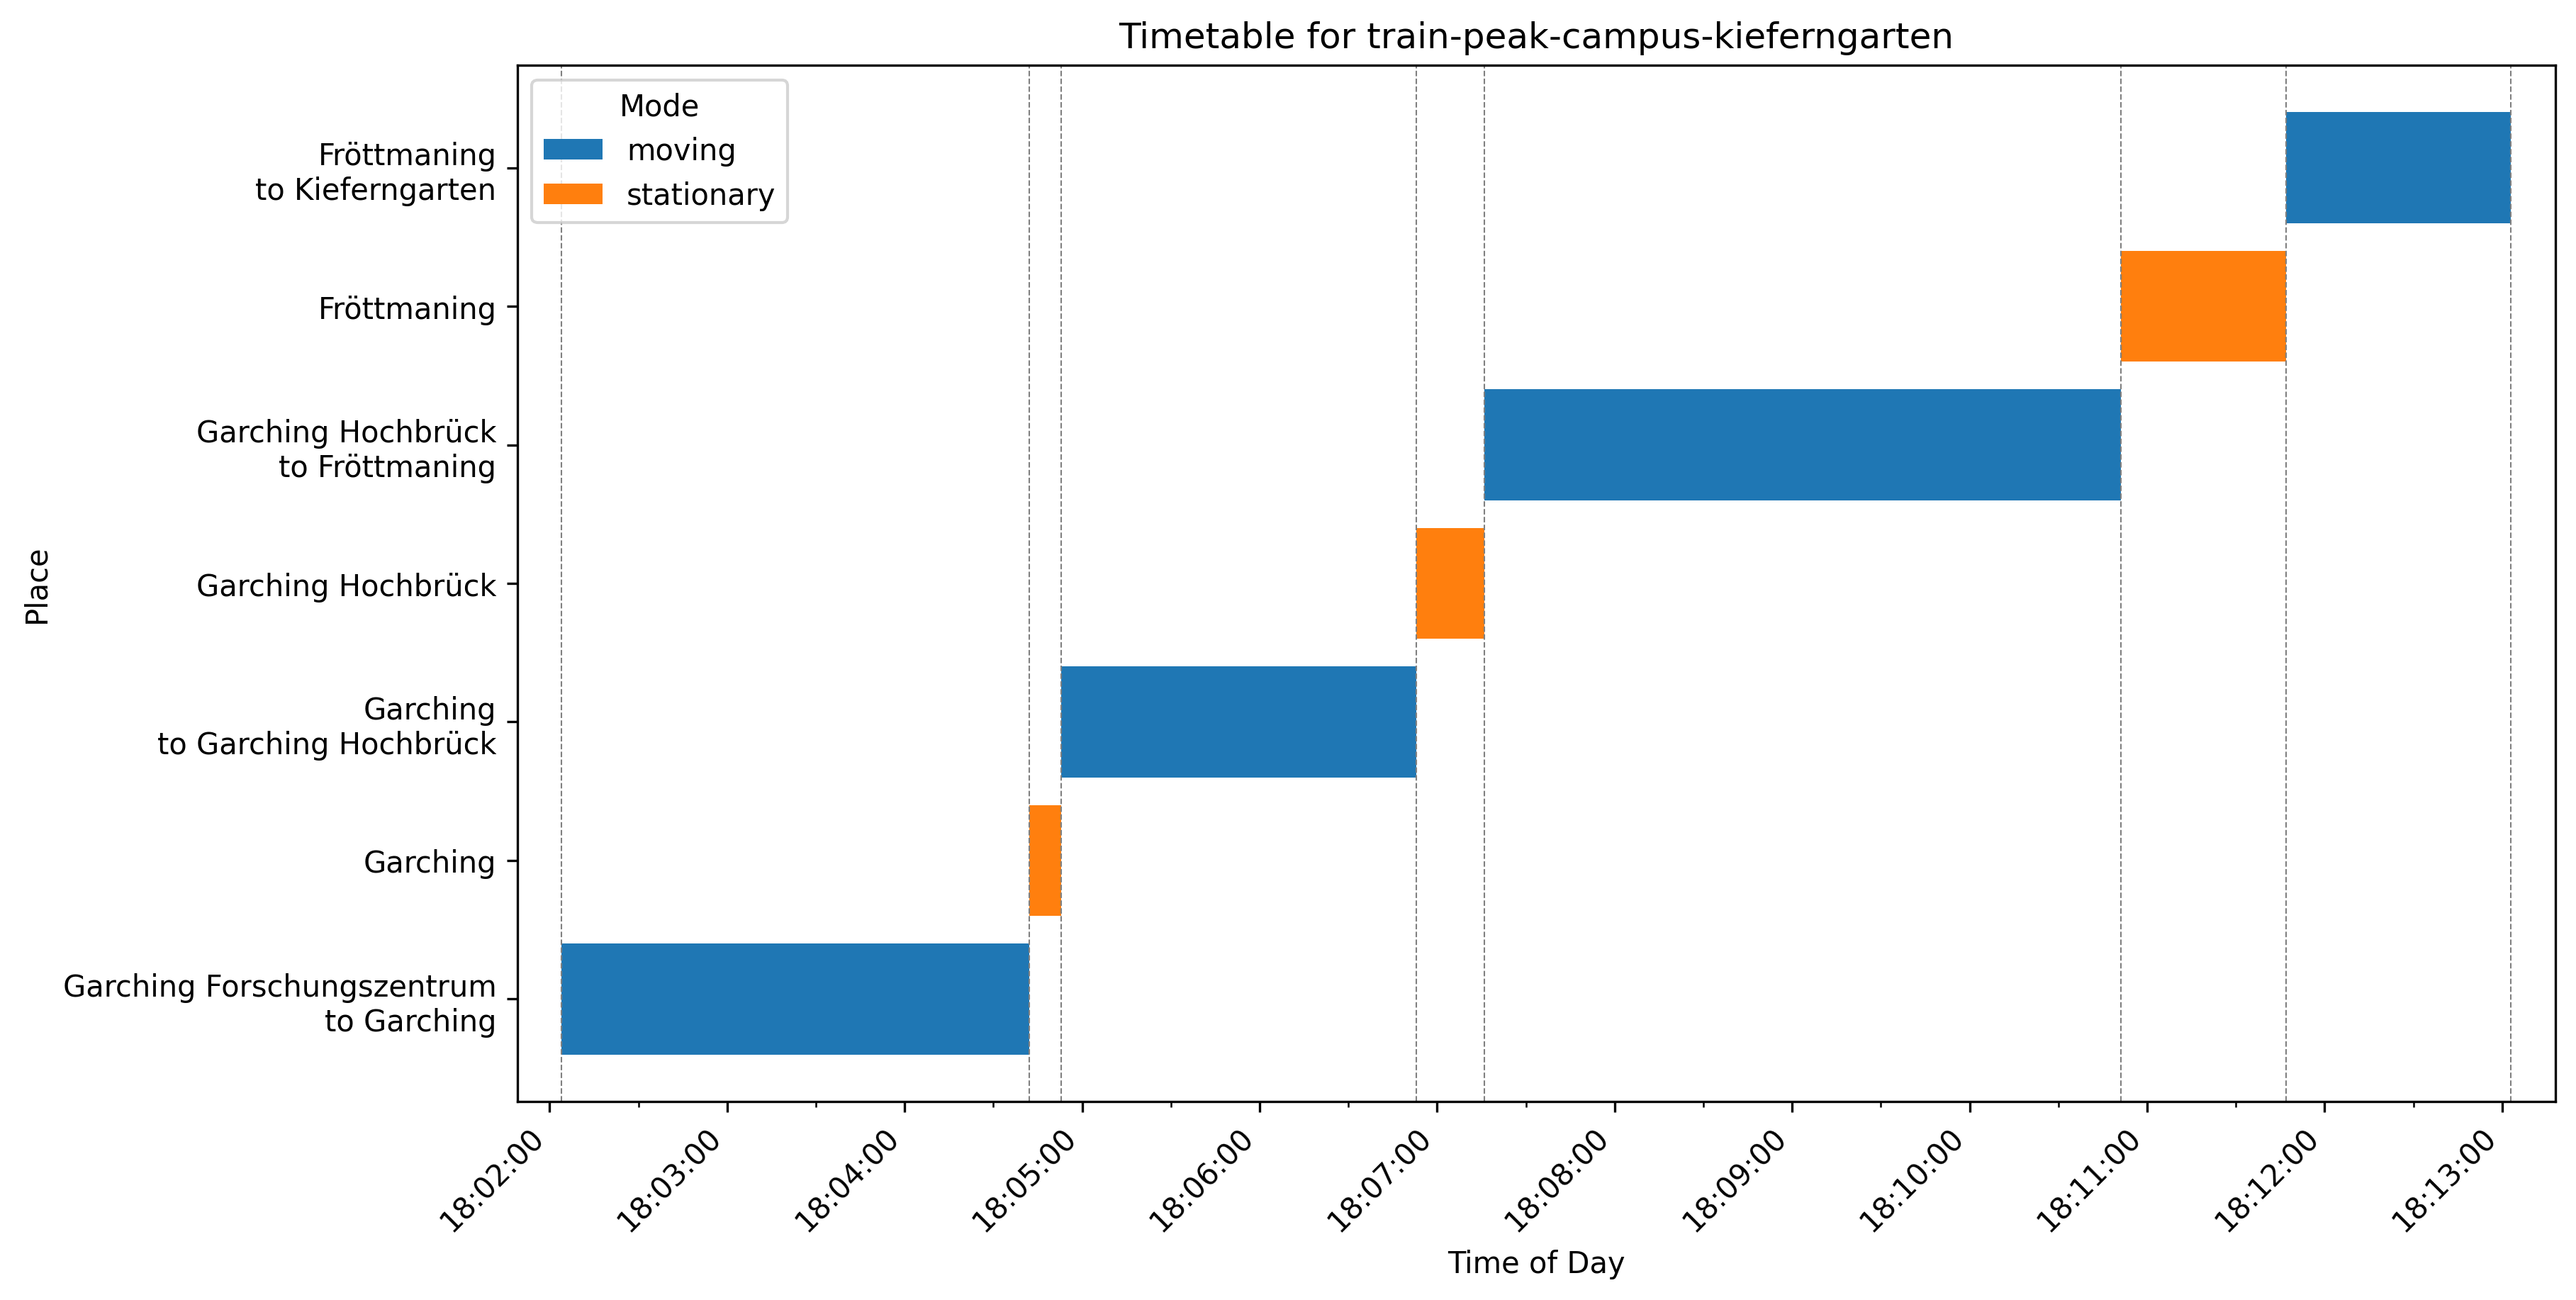
\includegraphics[width=\columnwidth]{images/part1/timetables/timetable-train-peak-campus-kieferngarten.png}
    \caption{Timetable for train-peak-campus-kieferngarten scenario}
    \label{fig:timetable-train-peak-campus-kieferngarten}
\end{figure}

\begin{figure}
    \centering
    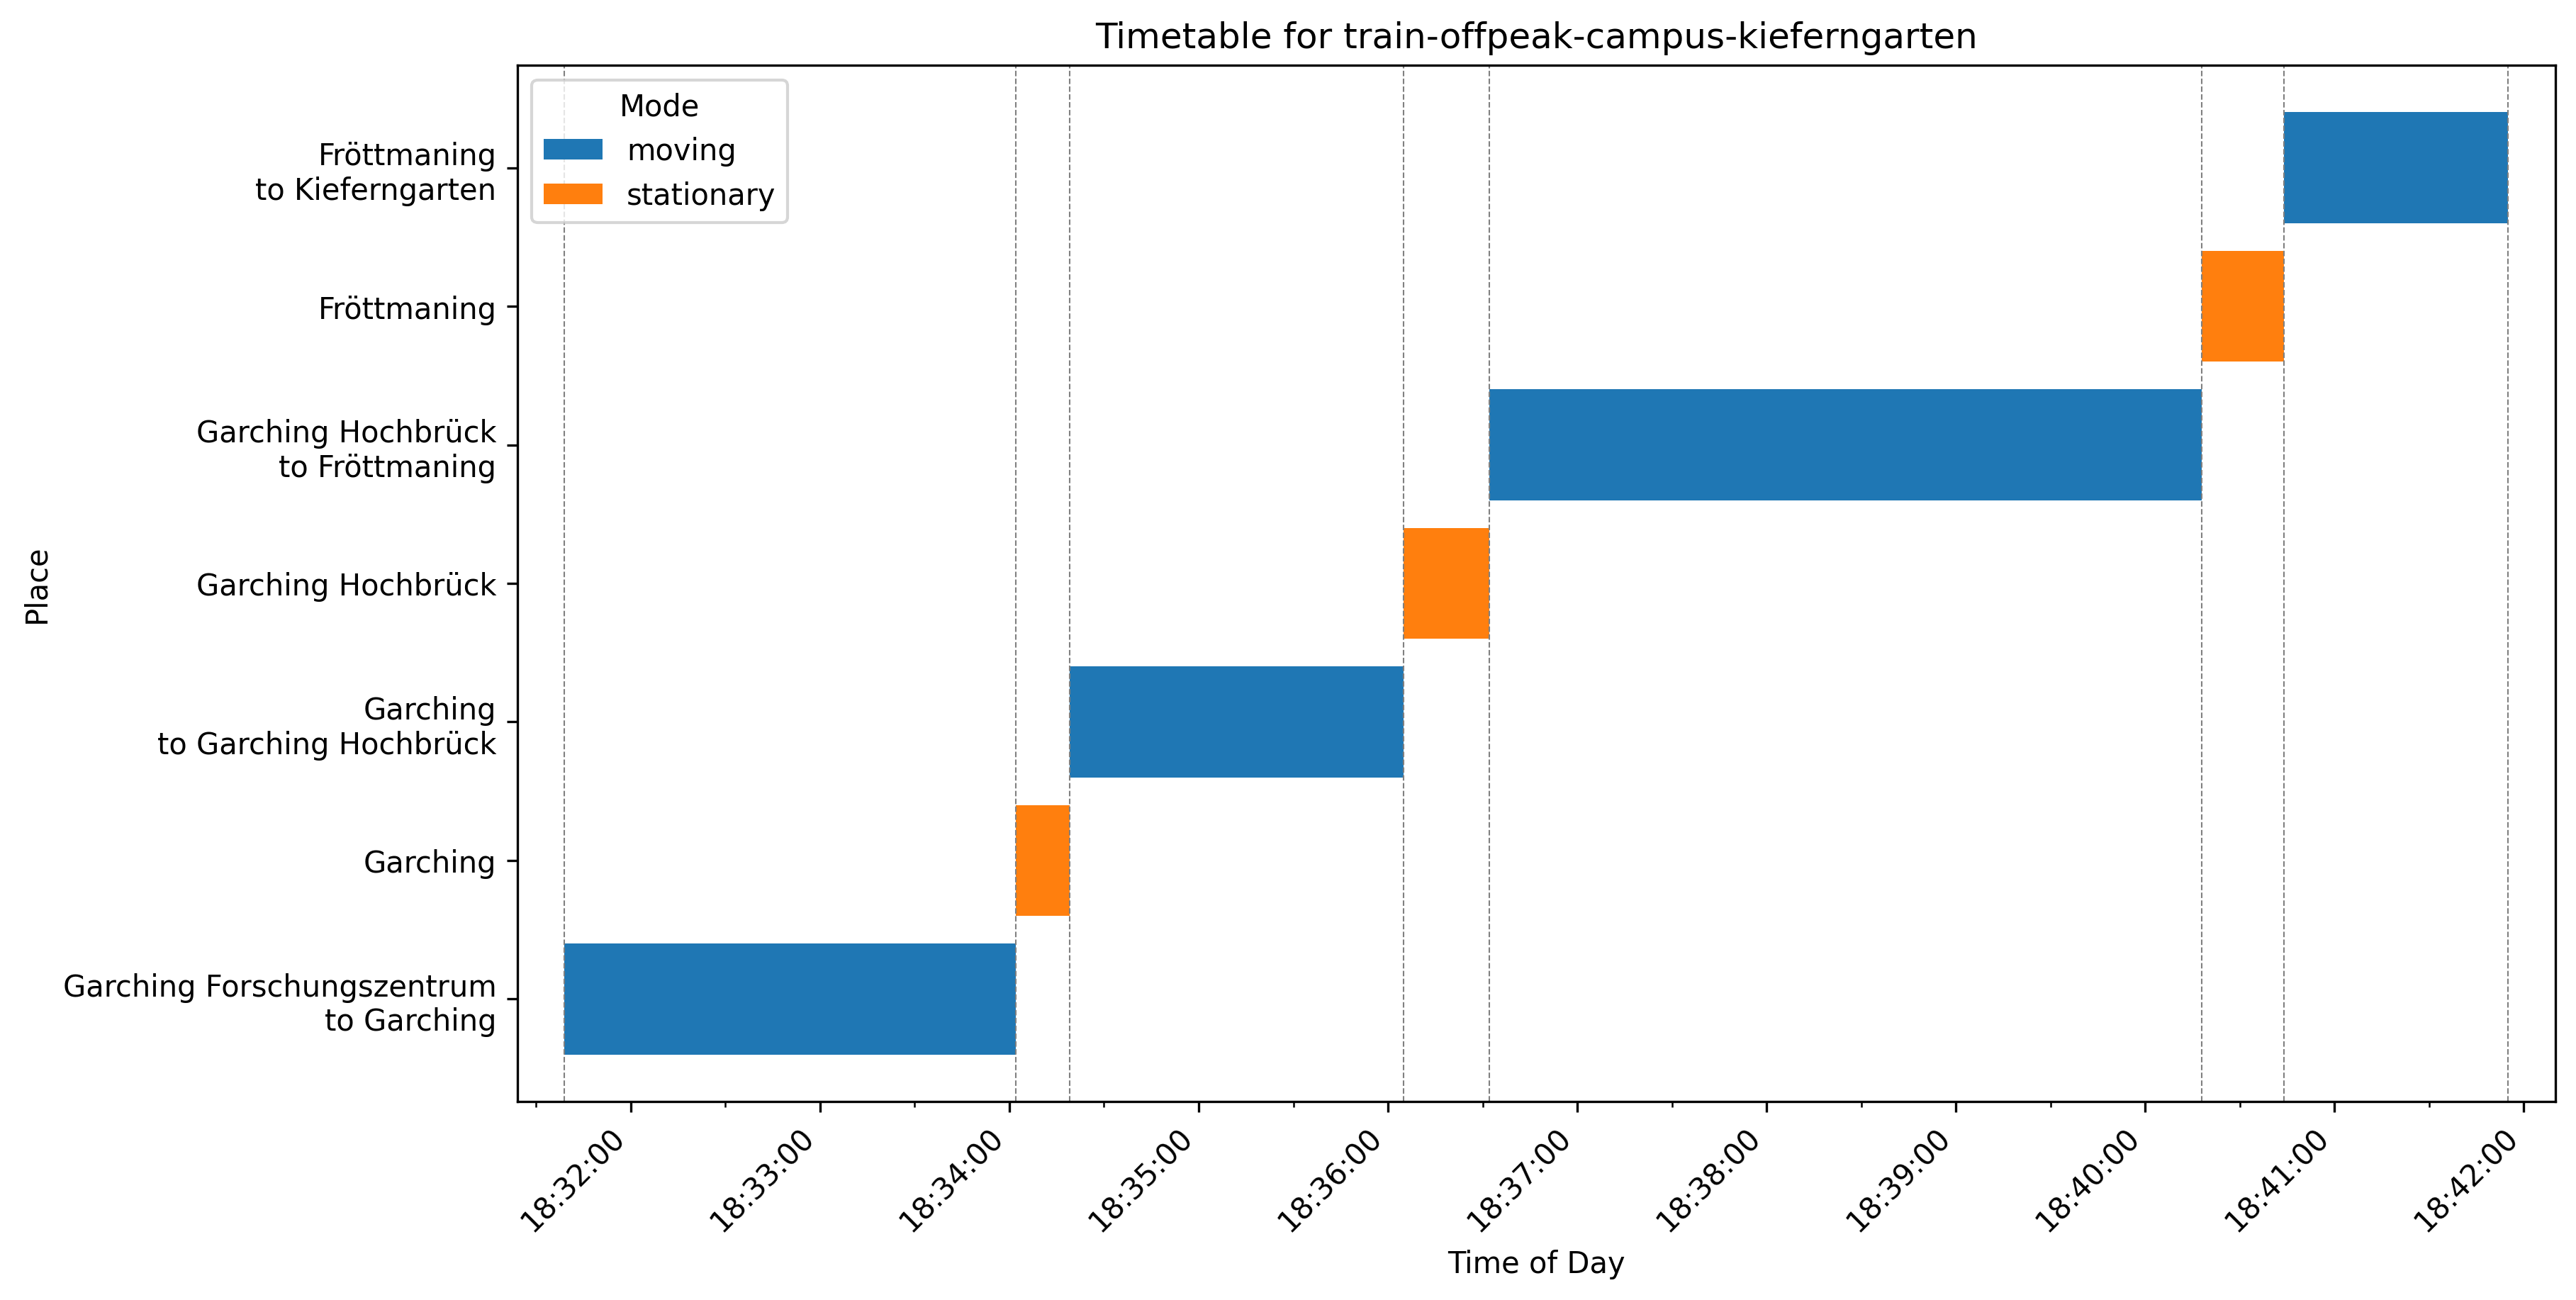
\includegraphics[width=\columnwidth]{images/part1/timetables/timetable-train-offpeak-campus-kieferngarten.png}
    \caption{Timetable for train-offpeak-campus-kieferngarten scenario}
    \label{fig:timetable-train-offpeak-campus-kieferngarten}
\end{figure}

\begin{figure}
    \centering
    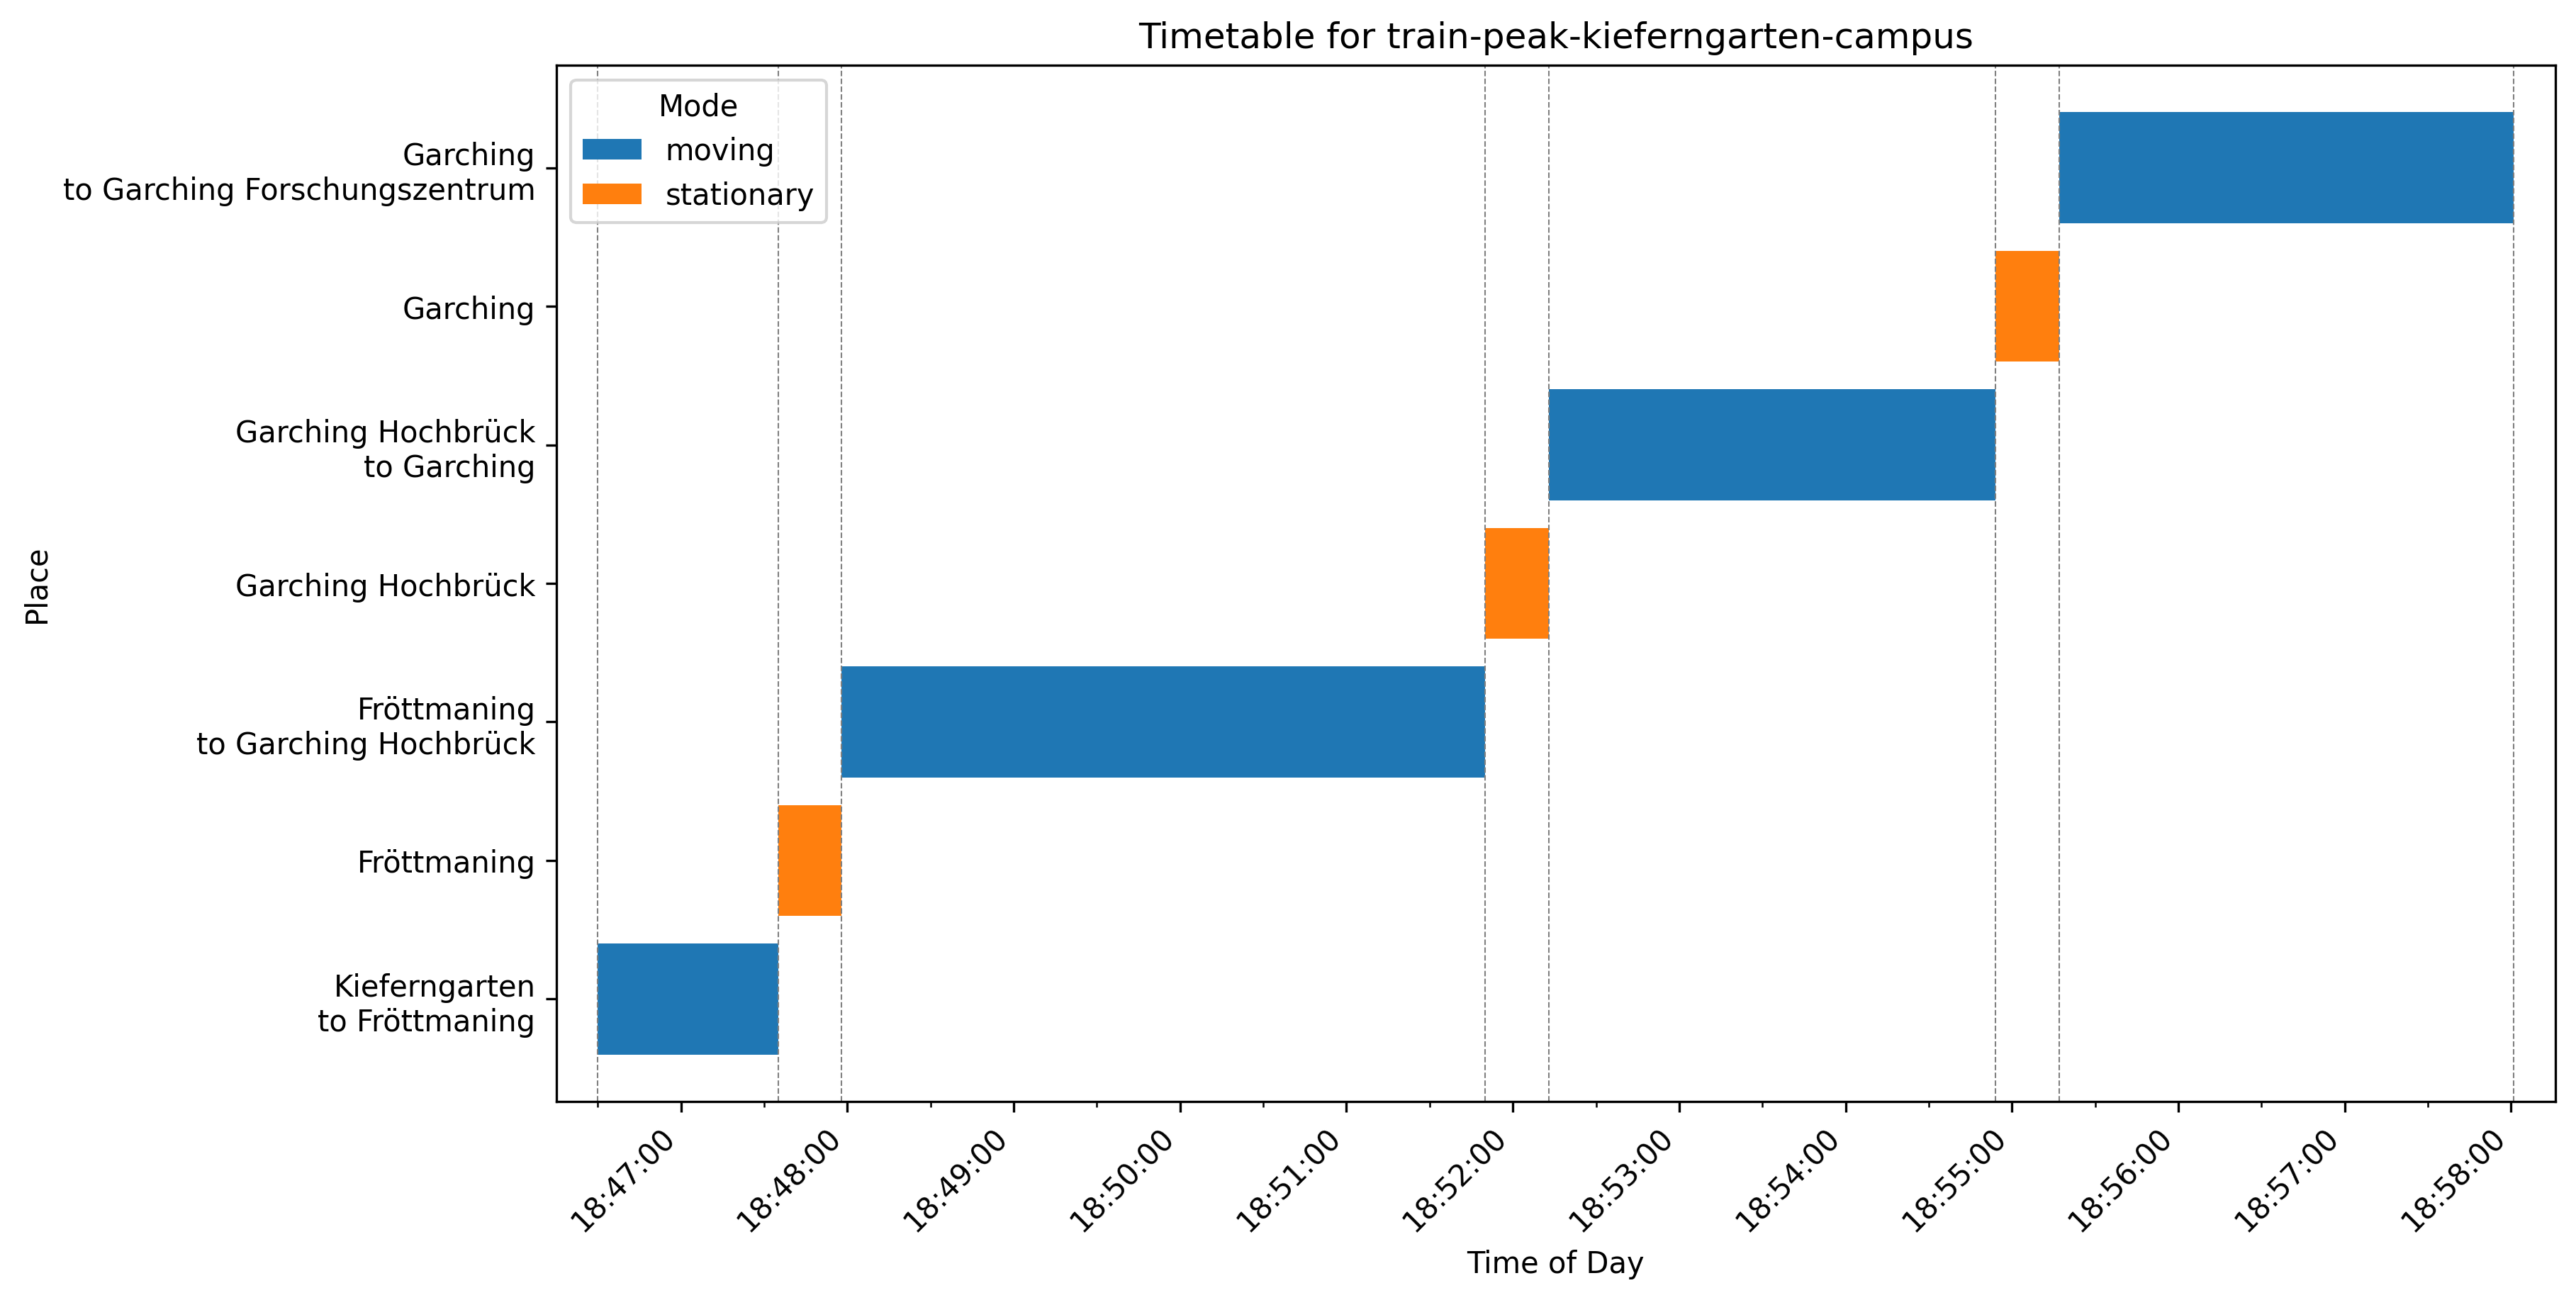
\includegraphics[width=\columnwidth]{images/part1/timetables/timetable-train-peak-kieferngarten-campus.png}
    \caption{Timetable for train-peak-kieferngarten-campus scenario}
    \label{fig:timetable-train-peak-kieferngarten-campus}
\end{figure}

\begin{figure}
    \centering
    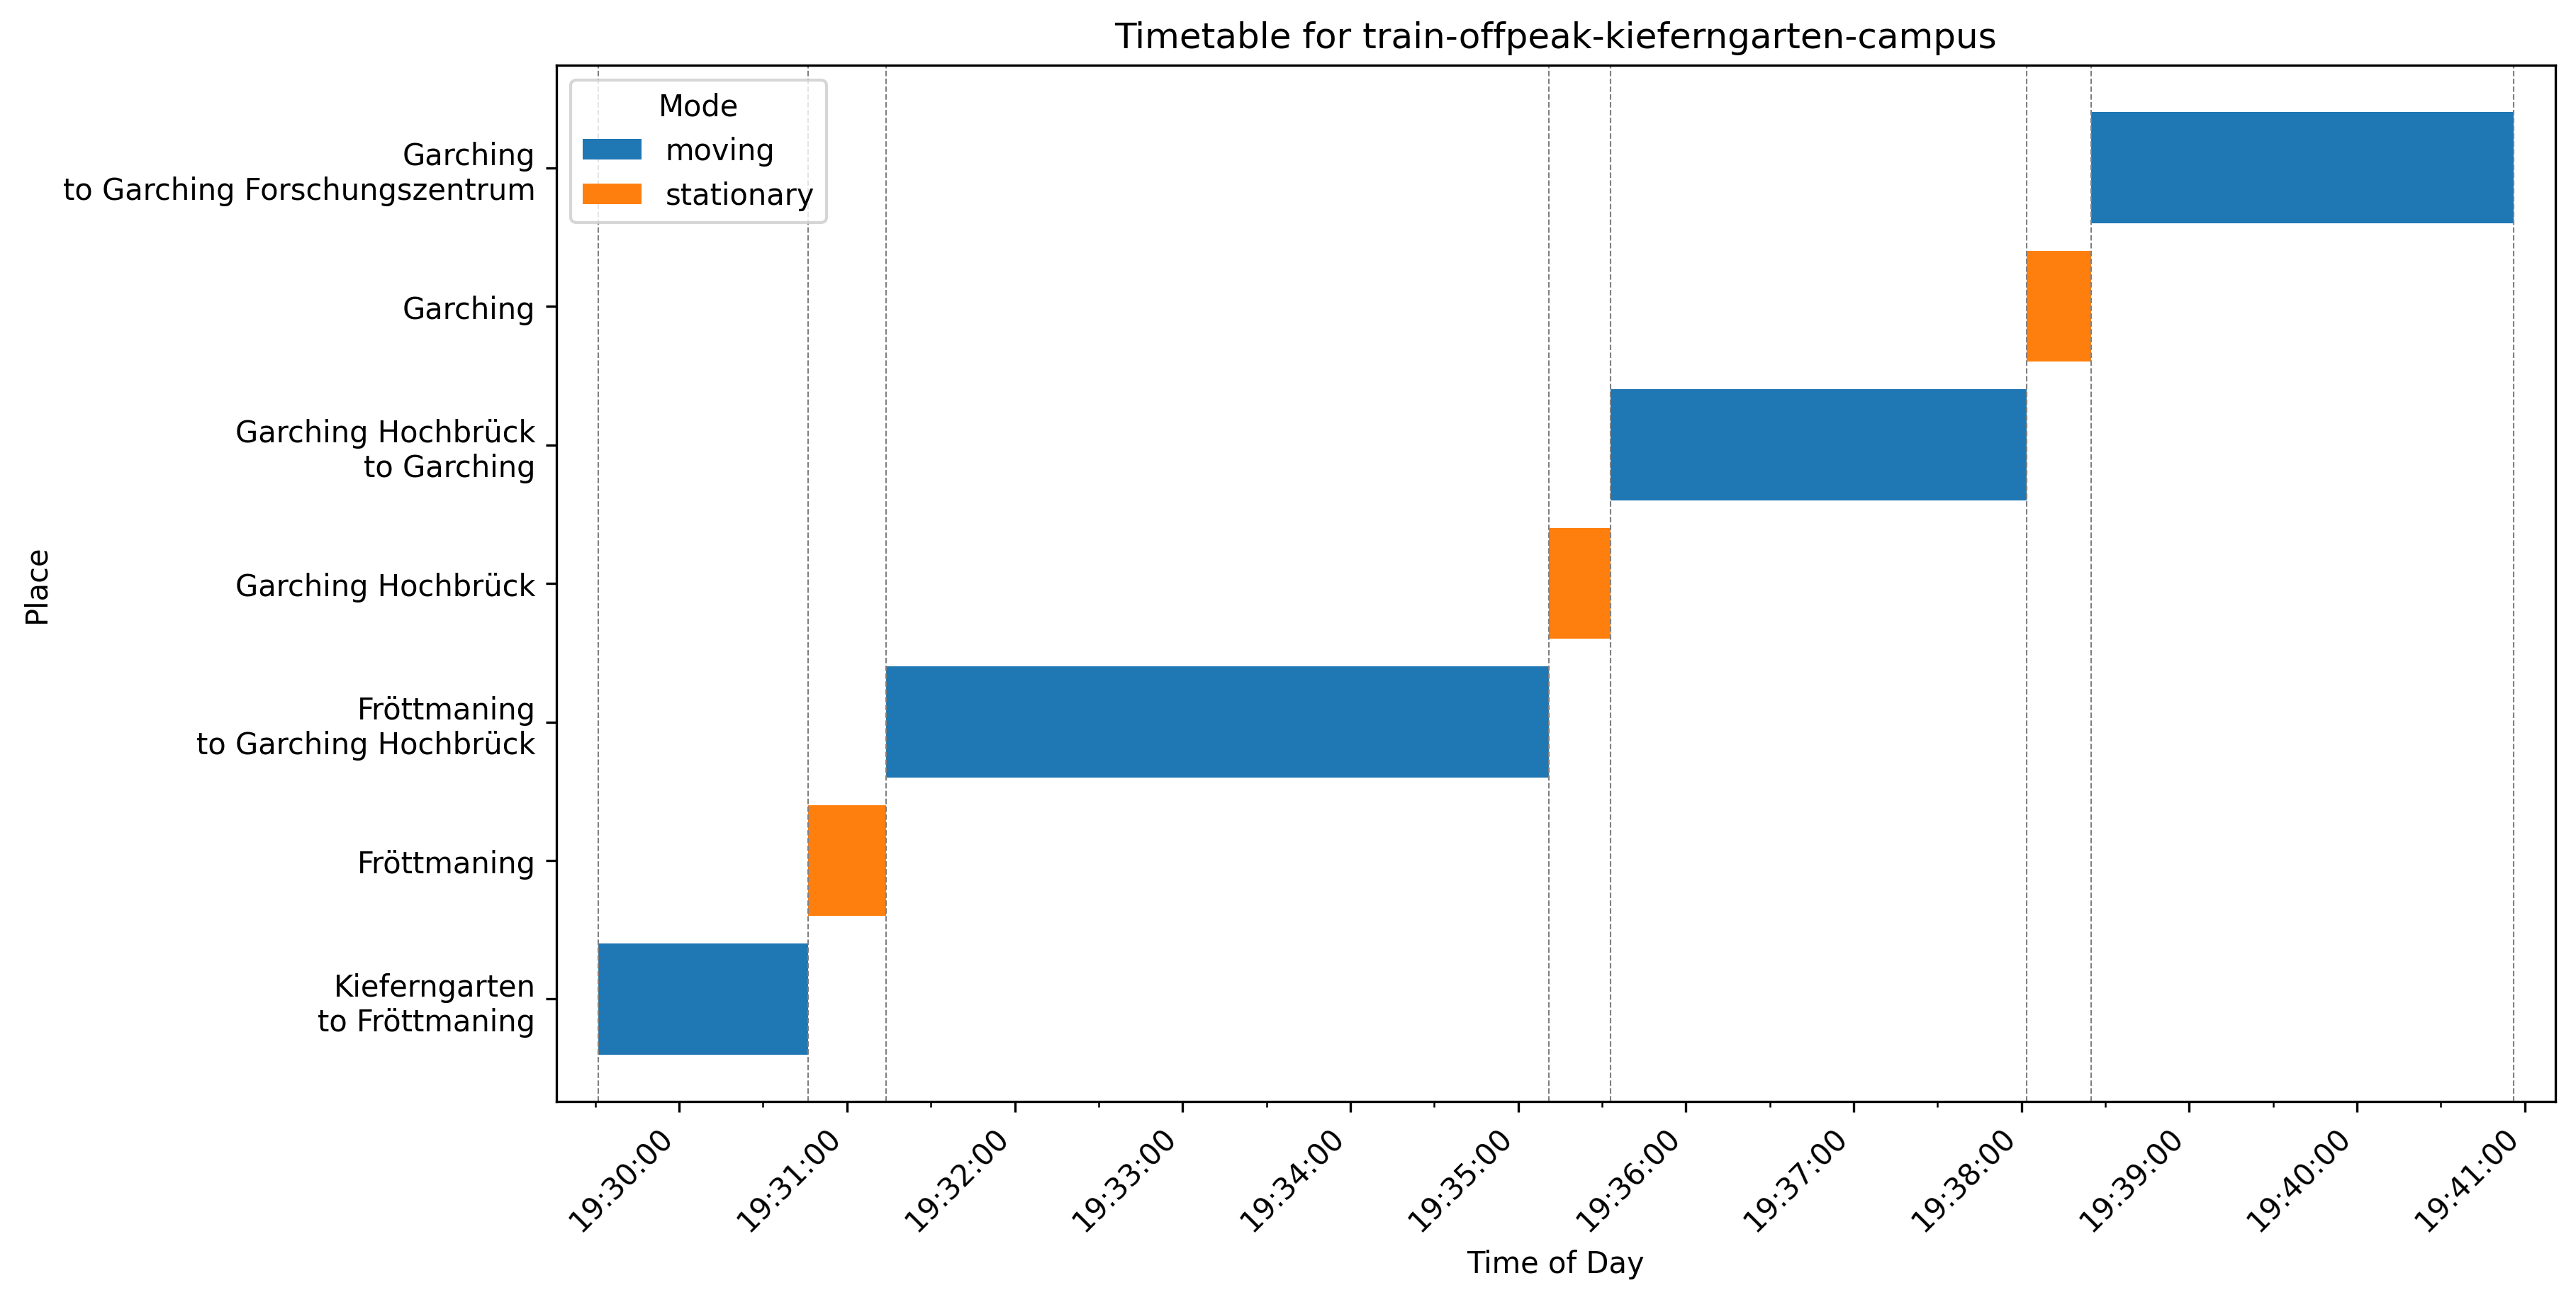
\includegraphics[width=\columnwidth]{images/part1/timetables/timetable-train-offpeak-kieferngarten-campus.png}
    \caption{Timetable for train-offpeak-kieferngarten-campus scenario}
    \label{fig:timetable-train-offpeak-kieferngarten-campus}
\end{figure}

\subsubsection{Involved Devices}
\label{sec:part-1/da-co/devices}
To control the capture process, we use a smartphone to be an AP, to which the Raspberry Pi (through wlan0, the interface of the integrated Wi-Fi device) and a laptop are connected. On all devices involved (Raspberry Pi, smartphone, and laptop), we disable MAC randomization to have better trackability of the devices closest to the capturing antennas. Both the smartphone and the laptop are then put into power-saving mode to reduce their influence on the capture by reducing the number of probe requests they send. Additionally, throughout the capture, the Raspberry Pi and the laptop stayed connected to the smartphone AP, which stopped the Raspberry Pi from sending probe requests altogether and reduced the probe request rate of the laptop even further.

\subsection{Analysis}
\label{sec:part-1/ana}

% What data analysis techniques are used to derive what information

\subsubsection{Noise Filtering}
\label{sec:part-1/ana/noise-filtering}
To filter out noise from the captured Probe Requests, we employed a simple packet filter. After capturing, in the preprocessing stage, we filter out probe requests with less than -70 dBm signal strength, as those probes would be from devices that are too far away to be considered in the same place/scenario.

\subsubsection{MAC Address Randomization}
\label{sec:part-1/ana/mac-randomization}

To identify random MAC addresses, we rely on the second significant bit of the first byte in the \textbf{Organizationally Unique Identifier (OUI)}. If this bit is set, it indicates that the MAC address is \textit{locally administrated}; otherwise, it is a \textit{globally unique} address. Since randomized MAC addresses are locally administered, the locally administered bit should be set to 1. \cite{cisco2022rcm}

\begin{figure}[h]
    \centering
    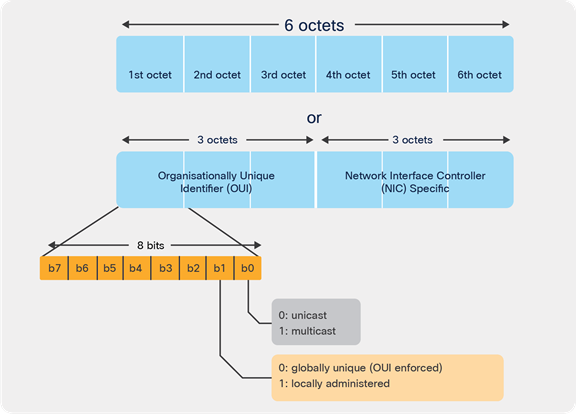
\includegraphics[width=\columnwidth]{images/randomized-changing-mac-dg_2.png}
    \caption{locally administrated MAC addresses are random MAC addresses \cite{cisco2022rcm}}
    \label{fig:random-mac-address}
\end{figure}

\subsubsection{Smoothing}
To smooth the packet arrival rates, we use Savitzky-Golay filtering \cite{savitzky1964smoothing}, which is a common technique to smooth time series data. The smoothing is done with a window size of 5 seconds and a polynomial order of 2.

\subsection{Results Overview}
\label{sec:part-1/res}

In this section and the following results sections, we present and discuss the results of varying scenarios. The results are presented in the form of plots and tables, which summarize the characteristics of the captured data.

\begin{table}[ht]
    \centering
    \resizebox{\columnwidth}{!}{
    \begin{tabular}{|>{\columncolor[gray]{0.95}}l|c|c|c|}
        \hline
        Scenario & Packet Count & Mean RSSI (dBm) & Std Dev RSSI (dBm) \\
        \hline
        \rowcolor[HTML]{EAF2FB} station-peak-campus & 6980 & -58.38 & 9.03 \\
        \hline
        \rowcolor[HTML]{EAF2FB} station-peak-kieferngarten & 11289 & -58.46 & 8.97 \\
        \hline
        \rowcolor[HTML]{F7F6D1} station-offpeak-campus & 1095 & -62.14 & 8.11 \\
        \hline
        \rowcolor[HTML]{F7F6D1} station-offpeak-kieferngarten & 4609 & -59.99 & 9.36 \\
        \hline
        \rowcolor[HTML]{DFF2DF} train-peak-campus-kieferngarten & 7654 & -48.61 & 11.67 \\
        \hline
        \rowcolor[HTML]{DFF2DF} train-peak-kieferngarten-campus & 1840 & -53.94 & 11.99 \\
        \hline
        \rowcolor[HTML]{F2EAFB} train-offpeak-campus-kieferngarten & 6737 & -60.13 & 7.18 \\
        \hline
        \rowcolor[HTML]{F2EAFB} train-offpeak-kieferngarten-campus & 3202 & -54.24 & 11.35 \\
        \hline
    \end{tabular}
    }
    \caption{Overview of Probe Frame Counts, and RSSI Distribution}
    \label{tab:probe_frame_overview}
\end{table}

As expected, it can clearly be seen that the peak scenarios have a significantly higher number of probe requests captured than the off-peak scenarios.

Additionally, the number of probe requests heavily favors Kieferngarten over Garching Forschungszentrum. This is due to the fact that Kieferngarten is closer to the city center, which intuitively makes it more likely to host more people. This difference is amplified even more due to the fact that there is a construction going on on the U-6 line, and Kieferngarten is the last station before the required transfer to the rest of the U-6 line, which makes even more people than normal to leave at the station or wait for the next train to arrive there.

However, we don't see a significant difference in the RSSI values between the scenarios, which can be explained by the fact that the length of the stations and the trains are more or less the same, which would result in a similar spatial distribution of people. We assume that in none of the scenarios, people were distributed differently from the other scenarios.

Additionally, as it will be visible in the following sections, we did not observe any preference towards or significant difference between channels 1, 6, and 11, which are the channels we used for the captures, and observed that all three channels are highly correlated with each other.

\subsubsection{Device Behavior}

Upon our investigation into the behavior of the devices we used to capture the probe requests and control the capture process, we observed the behaviors summarized in \cref{tab:device_behavior}.

\begin{table}[H]
    \centering
    \caption{Probe request behavior of the smartphone and the controller laptop with and without power saving mode.}
    \label{tab:device_behavior}
    \resizebox{\columnwidth}{!}{%
    \begin{tabular}{|l|l|l|}
        \hline
        \textbf{Device} & \textbf{Power Saving Enabled} & \textbf{Power Saving Disabled} \\
        \hline
        \textbf{Smartphone} & 
        \begin{tabular}[t]{@{}l@{}}
            - No probe requests (passive scanning only) \\
            - Bursts on Wi-Fi connection
        \end{tabular} &
        \begin{tabular}[t]{@{}l@{}}
            - Bursts every \textasciitilde180s \\
            - Bursts on Wi-Fi connection
        \end{tabular} \\
        \hline
        \textbf{Controller Laptop} &
        \begin{tabular}[t]{@{}l@{}}
            - Bursts every \textasciitilde600s \\
            - Bursts on Wi-Fi connection
        \end{tabular} &
        \begin{tabular}[t]{@{}l@{}}
            - Bursts every \textasciitilde60s \\
            - Bursts on Wi-Fi connection
        \end{tabular} \\
        \hline
    \end{tabular}
    }
\end{table}

The Raspberry Pi doesn't have a power-saving mode, and it doesn't send any probe requests when it is connected to a Wi-Fi network. Due to the fact that the Raspberry Pi will be connected to the smartphone AP at all times, we did not feel the need to investigate its behavior further.

\subsection{Results - Station Scenarios}
\label{sec:part-1/res-station}

\subsubsection{Crowd Estimations}
\label{sec:part-1/station/crowd-estimations}

The crowd estimations are done visually during the captures. 

For the crowd estimations of the stations, the estimated number of people is noted down at the beginning of the capture, when the train arrives at the station (only the train on the Garching Forschungszentrum - Kieferngarten line), and when the train leaves the station.

The crowd estimations can be found in \cref{tab:crowd_estimate-stations} and \cref{tab:crowd_estimate-trains}.

\begin{figure}
    \centering
    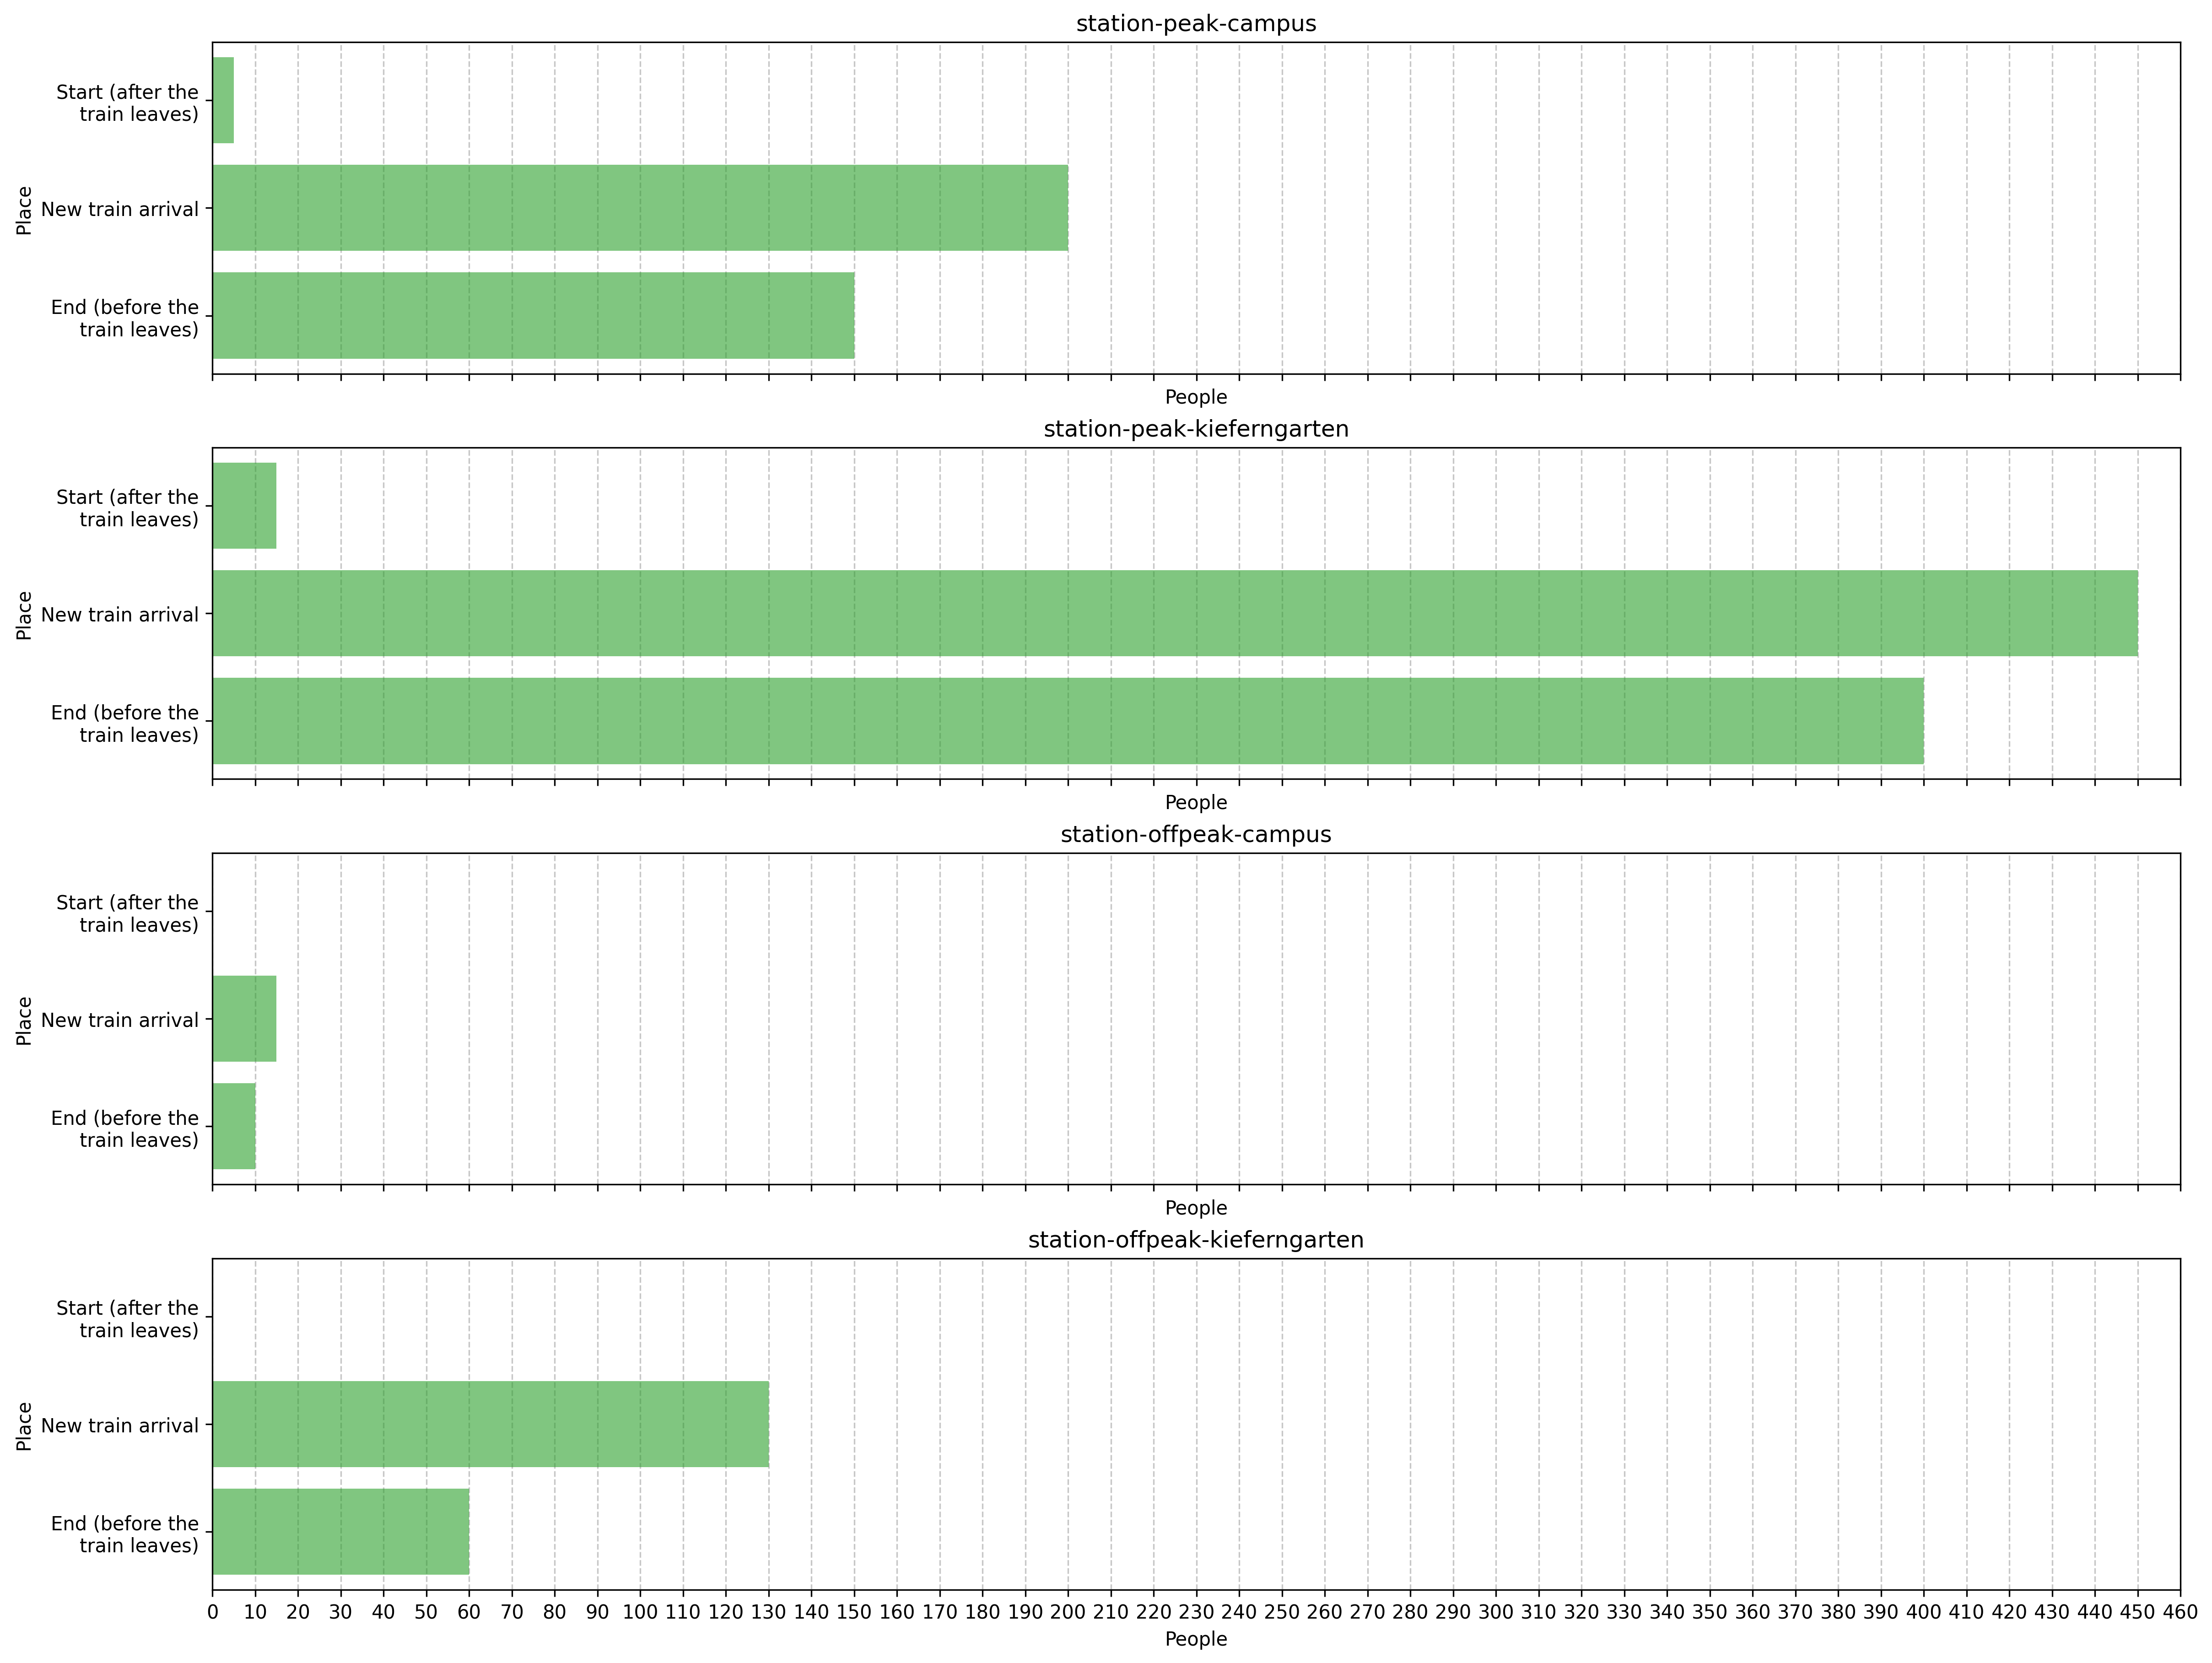
\includegraphics[width=\columnwidth]{images/part1/crowd-estimations/crowd-estimate-stations.png}
    \caption{Crowd Estimations for the Station Scenarios}
    \label{tab:crowd_estimate-stations}
\end{figure}

\subsubsection{Packet Counts}
\label{sec:part-1/station/packet-counts}

The cumulative packet counts and the packet arrival rates are shown in \cref{fig:station_cumulative_packet_counts} and \cref{fig:station_packet_arrival_rate}, respectively. The cumulative packet counts show the total number of packets captured over time, while the packet arrival rates show the number of packets captured per 5 seconds with the smoothing described in \cref{sec:part-1/ana/noise-filtering}.

\begin{figure}
    \centering
    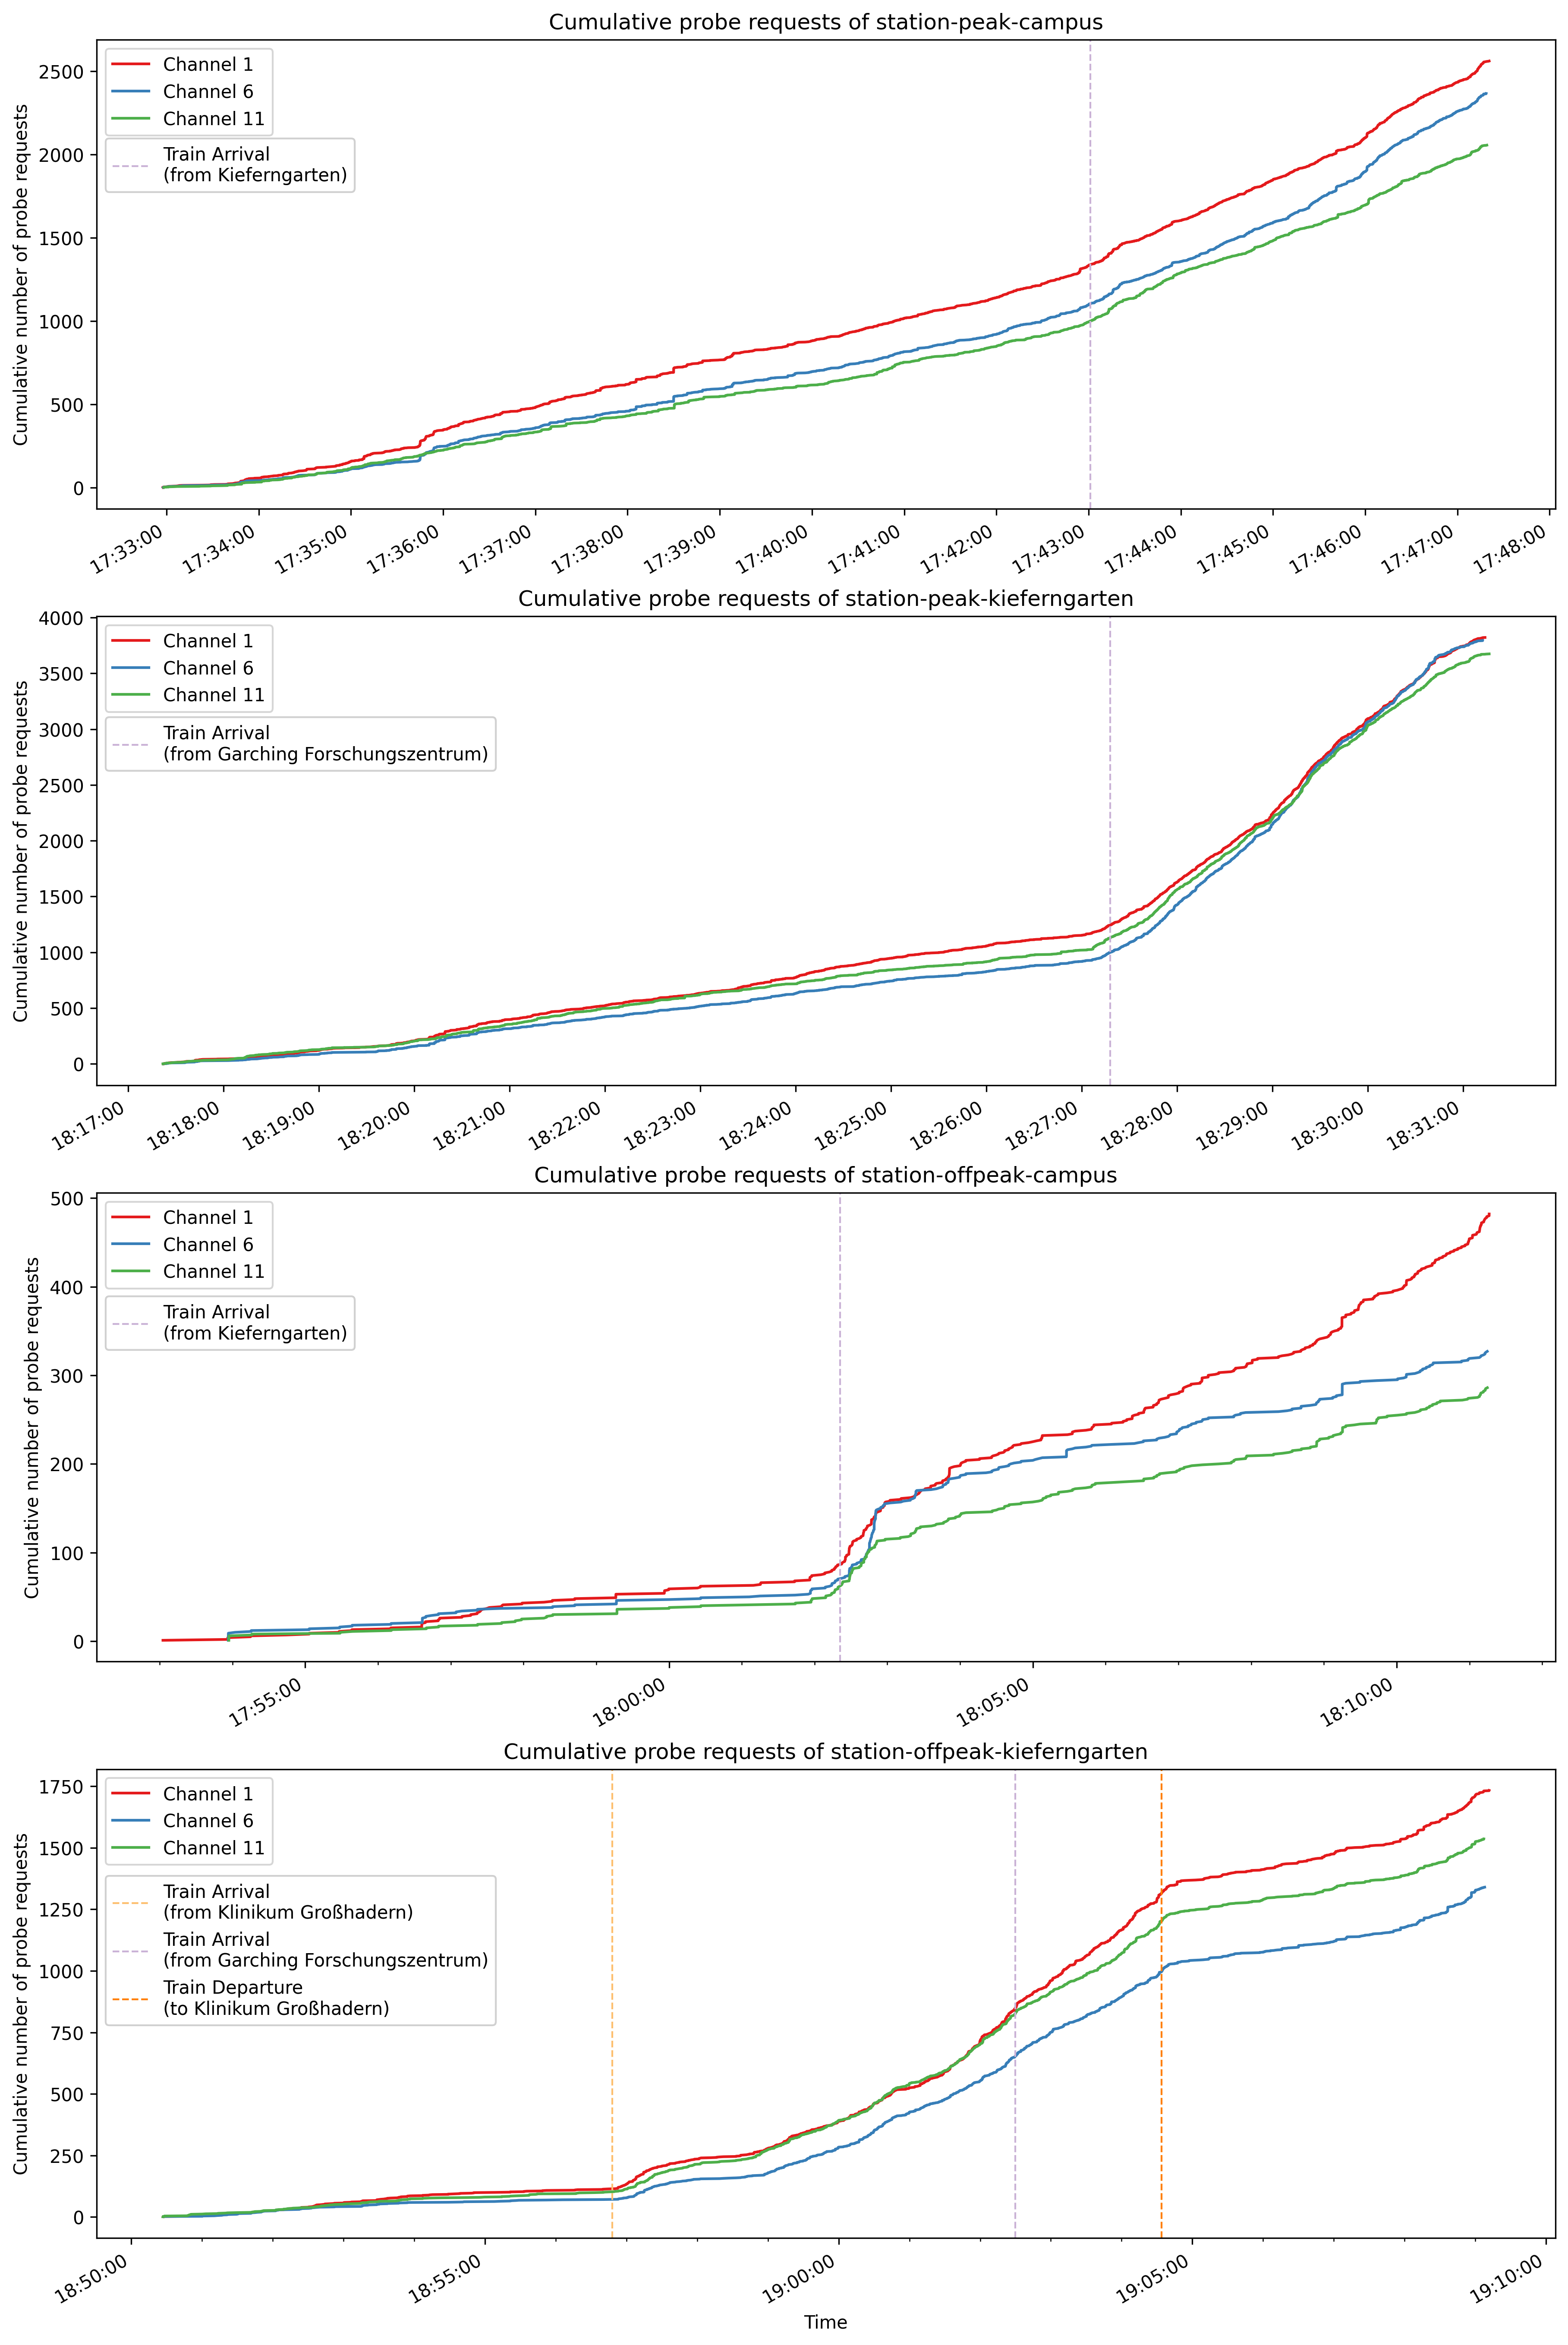
\includegraphics[width=\columnwidth]{images/part1/cumulative-packet-counts/station-scenarios.png}
    \caption{Cumulative Packet Counts for the Station Scenarios}
    \label{fig:station_cumulative_packet_counts}
\end{figure}

\begin{figure}
    \centering
    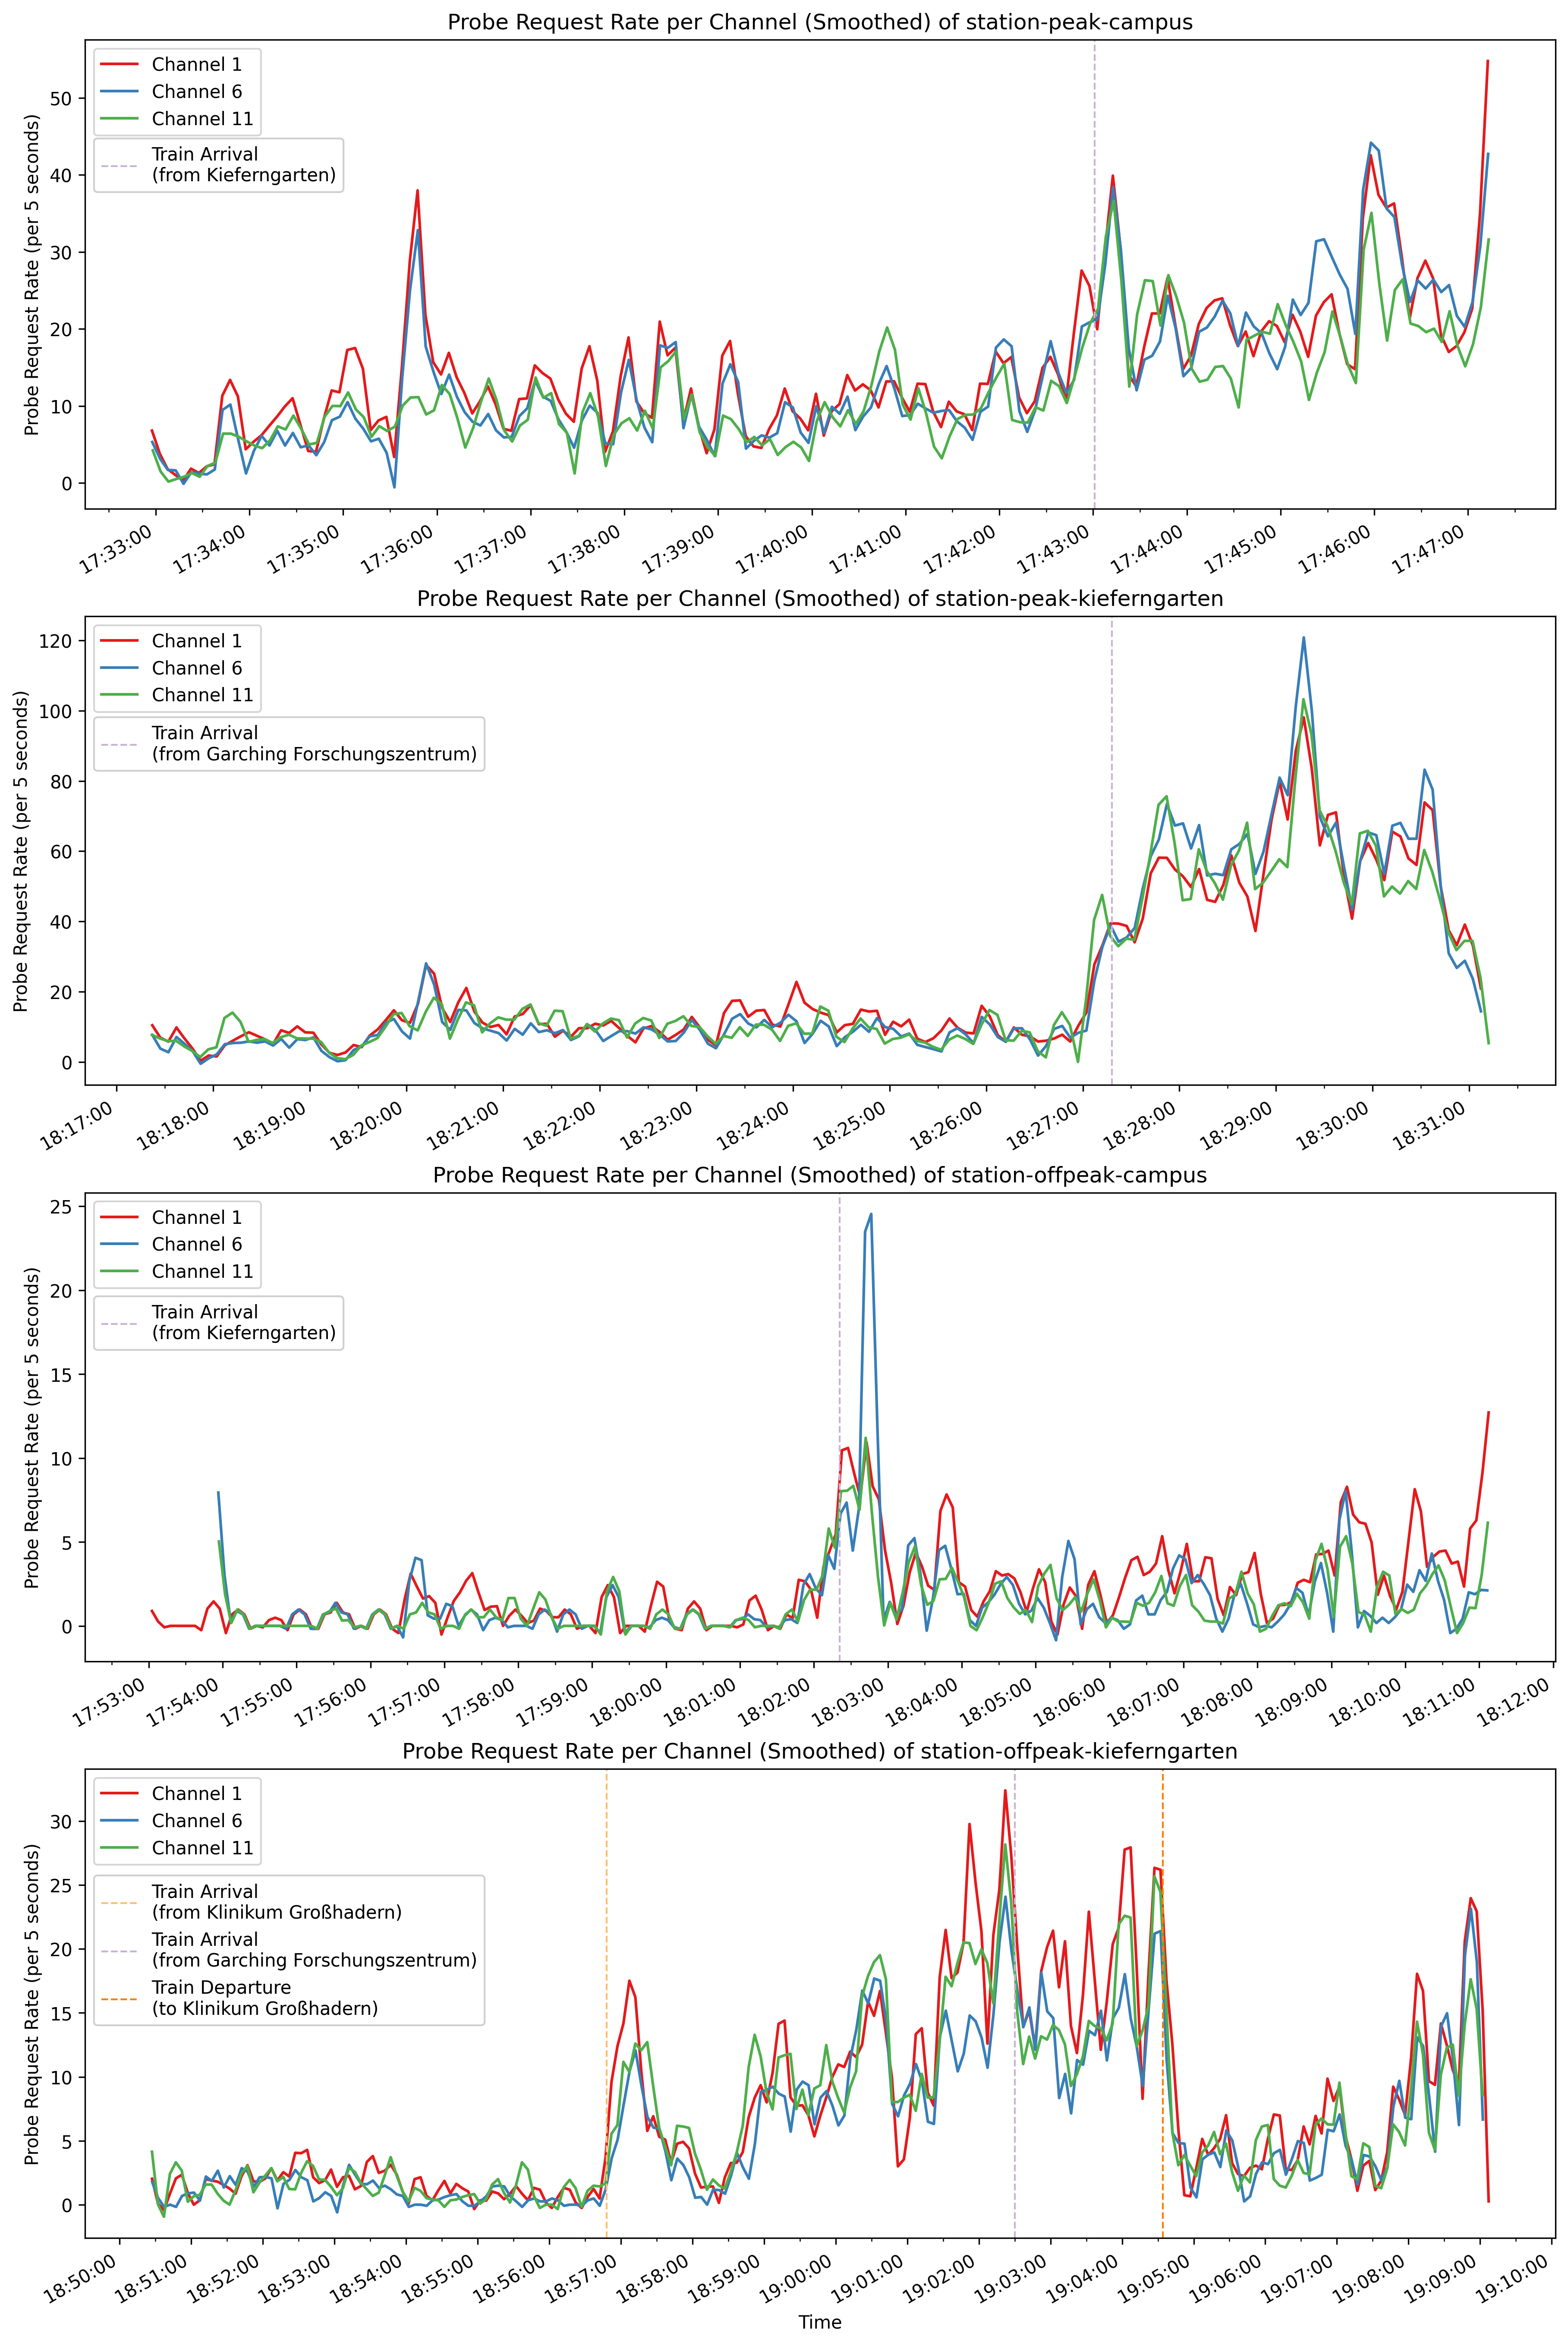
\includegraphics[width=\columnwidth]{images/part1/probe-rate/station-scenarios.png}
    \caption{Packet Arrival Rates for the Station Scenarios}
    \label{fig:station_packet_arrival_rate}
\end{figure}

As can be seen, the arrival of the next train at the station causes a significant increase in the number of packets captured, as more people arrive at the station all at once. This effect is less pronounced in the peak hours of the campus station (around 17:00 to 18:00 in the evening) corresponds to a time in the day when not a lot of people are arriving at the campus, which is why the increase in probe request rate is not as significant as in the other scenarios.

Additionally, the decrease in the probe request rate after the train leaves the station in the off-peak Kieferngarten station displays how people leaving affects the probe request rate pretty clearly. However, an additional train arriving and leaving cannot be observed at the campus station, as it is the terminal station. Unfortunately, an additional train (other than the one going back to the campus) arriving and leaving at the Kieferngarten station could not be observed in the peak scenario as well, due to the fact that it didn't coincide with the capture time.

Although slightly visible in the cumulative packet counts figures (\cref{fig:station_cumulative_packet_counts}) with a downturned bend after the train arrival events, the effect of people who arrived via the train leaving the station is much more visible in the packet arrival rates (\cref{fig:station_packet_arrival_rate}), where the probe request rate drops significantly after the sharp increase in the rate at a train arrival event. If people were to remain at the station after the train left, we would expect the probe request rate to remain high after the peak, but we see that the rate drops. However, this effect is not as pronounced in the Kieferngarten station as people are moving from one train to the other due to the transfer status of the station, which is why the probe request rate doesn't drop as significantly as in the campus station scenarios.

Finally, both in the cumulative packet counts (\cref{fig:station_cumulative_packet_counts}) and the packet arrival rates (\cref{fig:station_packet_arrival_rate}), we can clearly identify the peak and off-peak scenarios, as the peak scenarios display higher packet counts and arrival rates than the off-peak scenarios.

\subsubsection{Packet Counts per MAC Address}
\label{sec:part-1/station/packet-counts-per-mac}

After observing the time series of the packet counts and arrival rates, we now turn our focus to the packet counts per MAC address. The packet counts per top 20 MAC addresses (with respect to the total packet counts) are shown in \cref{fig:station_packet_counts_per_mac}.

We also present the number of probe requests sent by the known devices (i.e., the devices we used to control the capture process) in \cref{tab:known_devices_station}.

\begin{table}[ht]
    \centering
    \resizebox{\columnwidth}{!}{
        \begin{tabular}{|l|ccc|}
            \hline
            \textbf{Scenario} & \textbf{Controller Laptop} & \textbf{Smartphone} & \textbf{Raspberry Pi} \\
            \hline
            station-peak-campus & 1 & 0 & 0 \\
            \hline
            station-peak-kieferngarten & 6 & 0 & 0 \\
            \hline
            station-offpeak-campus & 12 & 0 & 0 \\
            \hline
            station-offpeak-kieferngarten & 3 & 0 & 0 \\
            \hline
        \end{tabular}
    }
    \caption{Packet counts of known devices in station scenarios.}
    \label{tab:known_devices_station}
\end{table}

\begin{figure}
    \centering
    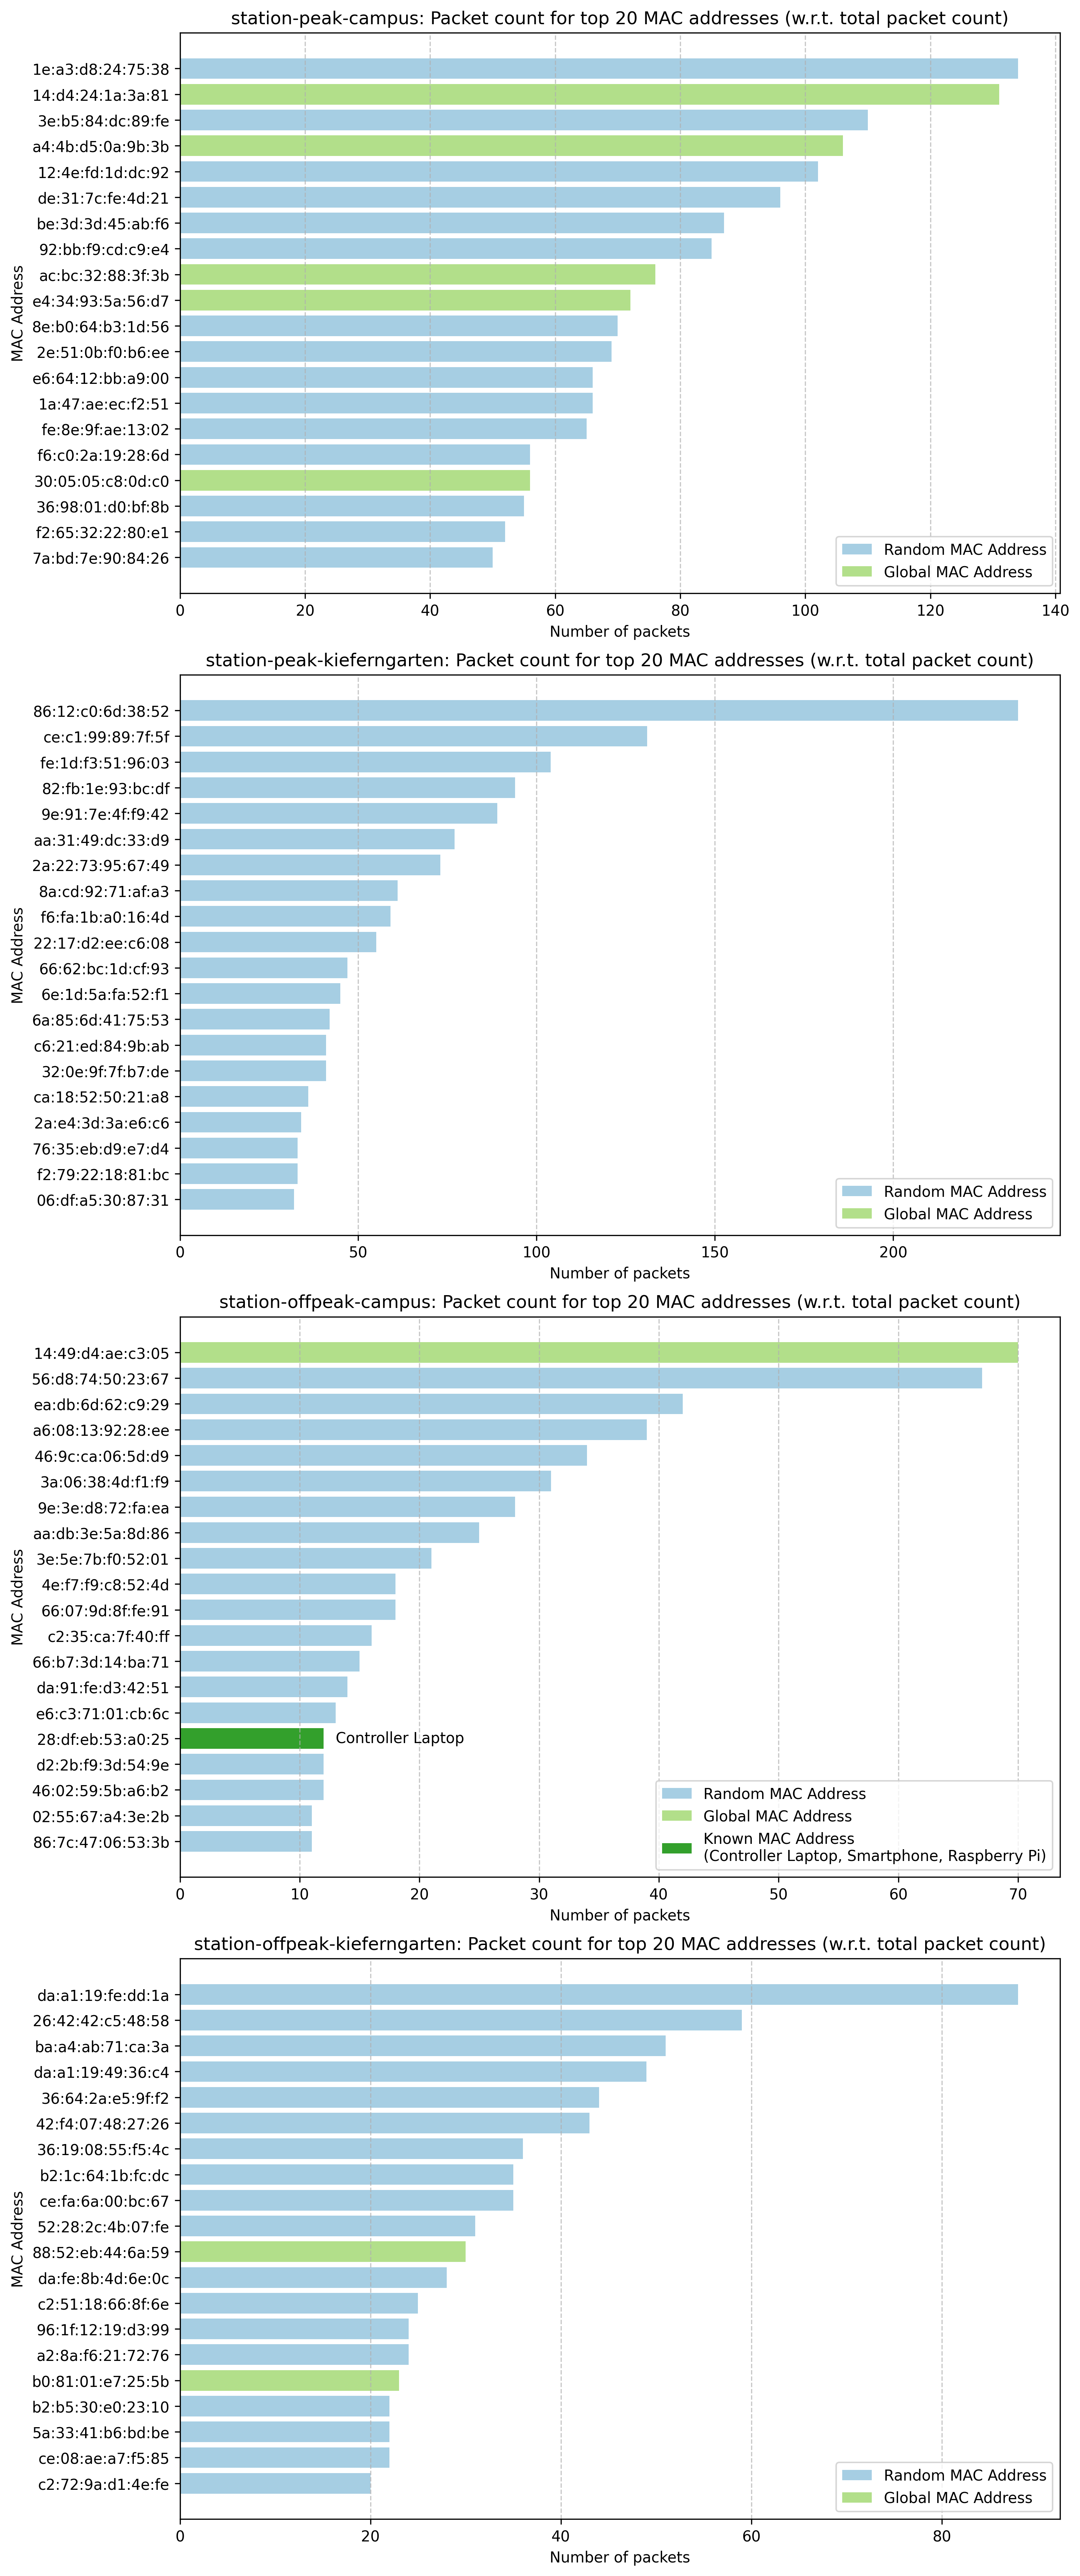
\includegraphics[width=\columnwidth]{images/part1/packet-counts/top-macs-station-scenarios.png}
    \caption{Packet Counts per MAC Address for the Station Scenarios}
    \label{fig:station_packet_counts_per_mac}
\end{figure}

Just like the cumulative statistics before, we can easily identify the peak and off-peak scenarios, as the top MAC addresses in the peak scenarios have significantly higher packet counts than the off-peak scenarios. This might seem obvious at first glance, but it is unintuitive when examined carefully, as the number of packets a device sends is not directly correlated with the number of people present at the station. Therefore, it is surprising that we see more packets from the top MAC addresses in the peak scenarios than in the off-peak scenarios. This is likely due to the fact that more people are present at the station, which increases the likelihood of a device that sends probe requests more frequently being present.

\subsubsection{RSSI Distribution}
\label{sec:part-1/station/rssi-distribution}

The RSSI distribution for the station scenarios is shown in \cref{fig:station_rssi_distribution}.

\begin{figure}
    \centering
    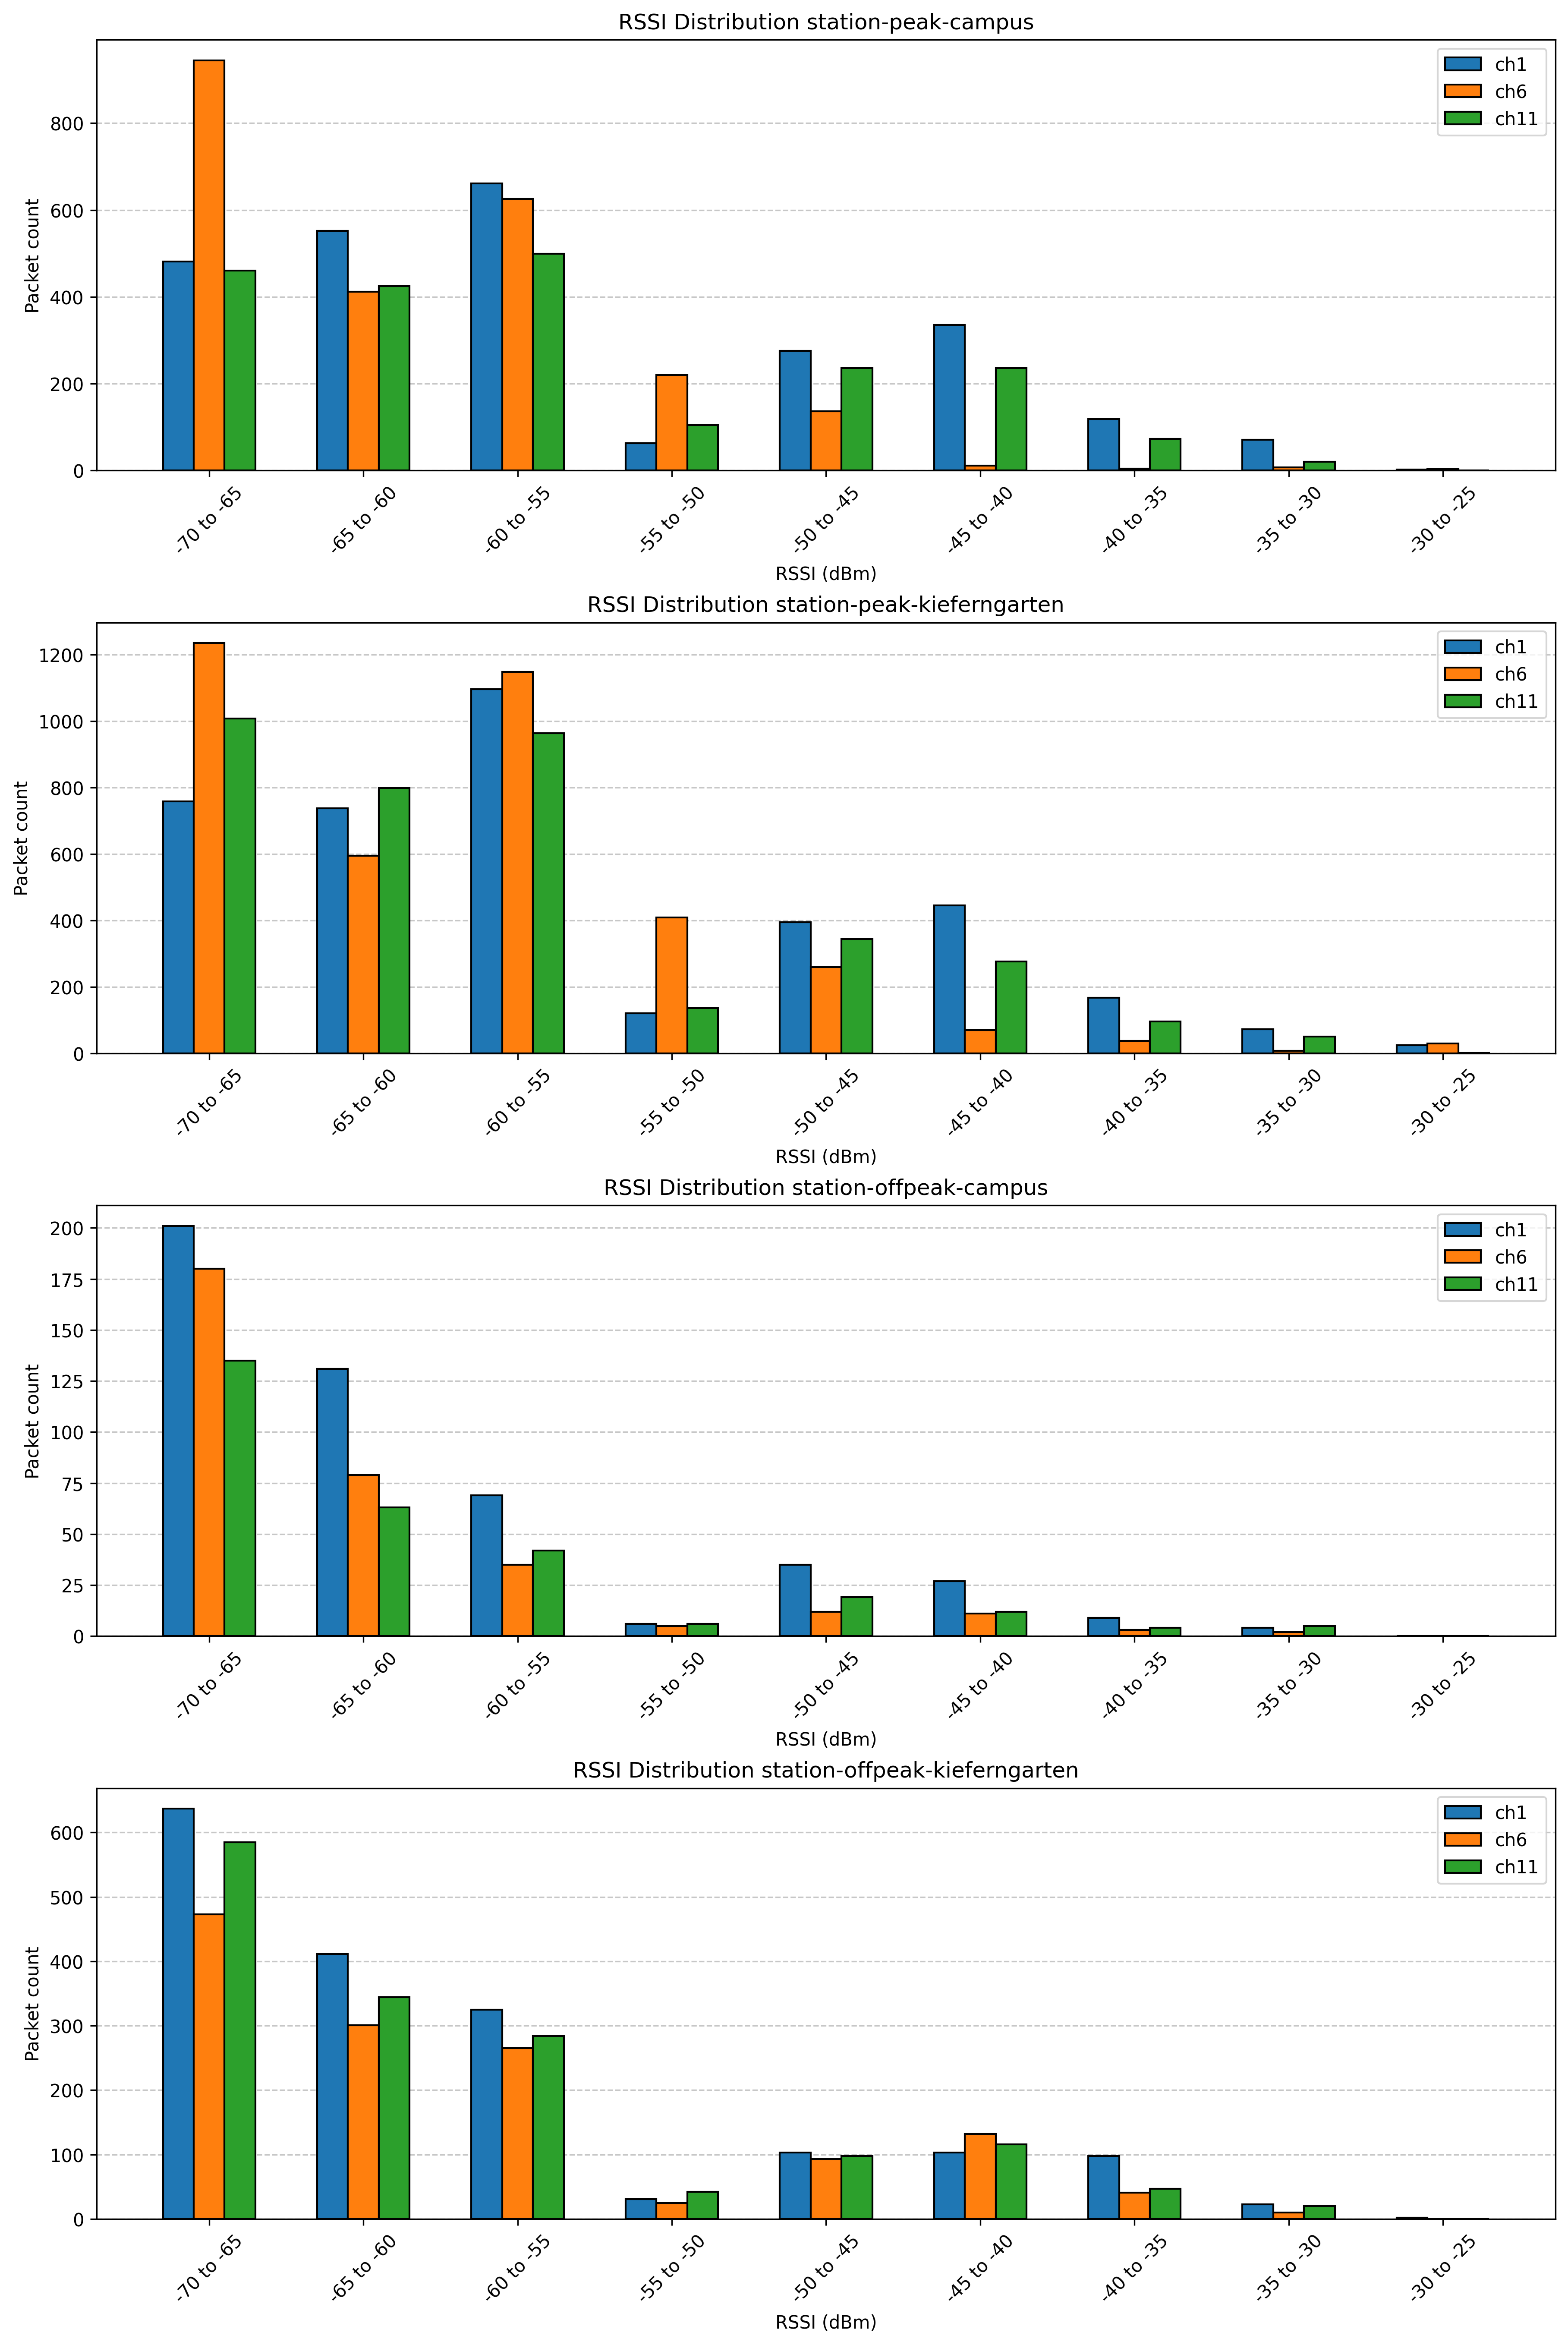
\includegraphics[width=\columnwidth]{images/part1/rssi/station-scenarios.png}
    \caption{RSSI Distribution for the Station Scenarios}
    \label{fig:station_rssi_distribution}
\end{figure}

In the station scenarios, we see a small dip in the RSSI distribution around -50 to -55 dBm. Using the log-distance path loss formula, we estimate that the -50 to -55 dBm range corresponds to 3 to 5 meters away (line of sight) from the antennas. This distance is less than the distance between the benches in the station, which led us to hypothesize that the gap is caused by people mainly gathering around the benches and not many people being present (comparatively) between the benches. Additionally, there is a concrete stairwell next to the middle bench at the Garching Forschungszentrum station, which could also cause a dip in the RSSI distribution as people cannot wait there. However, we did not test this hypothesis, as we did not have the time to capture the RSSI distribution at different locations in the station.

\subsubsection{RSSI Distribution per MAC Address}
\label{sec:part-1/station/rssi-distribution-per-mac}

We now turn our attention to the RSSI distribution per MAC address in hopes of finding out some patterns in the RSSI distribution of the known MAC addresses (i.e., the devices we used to control the capture process). The RSSI distribution per MAC address is shown in \cref{fig:station_rssi_distribution_per_mac}. We filter out the MAC addresses that sent less than 5 packets

\begin{figure}
    \centering
    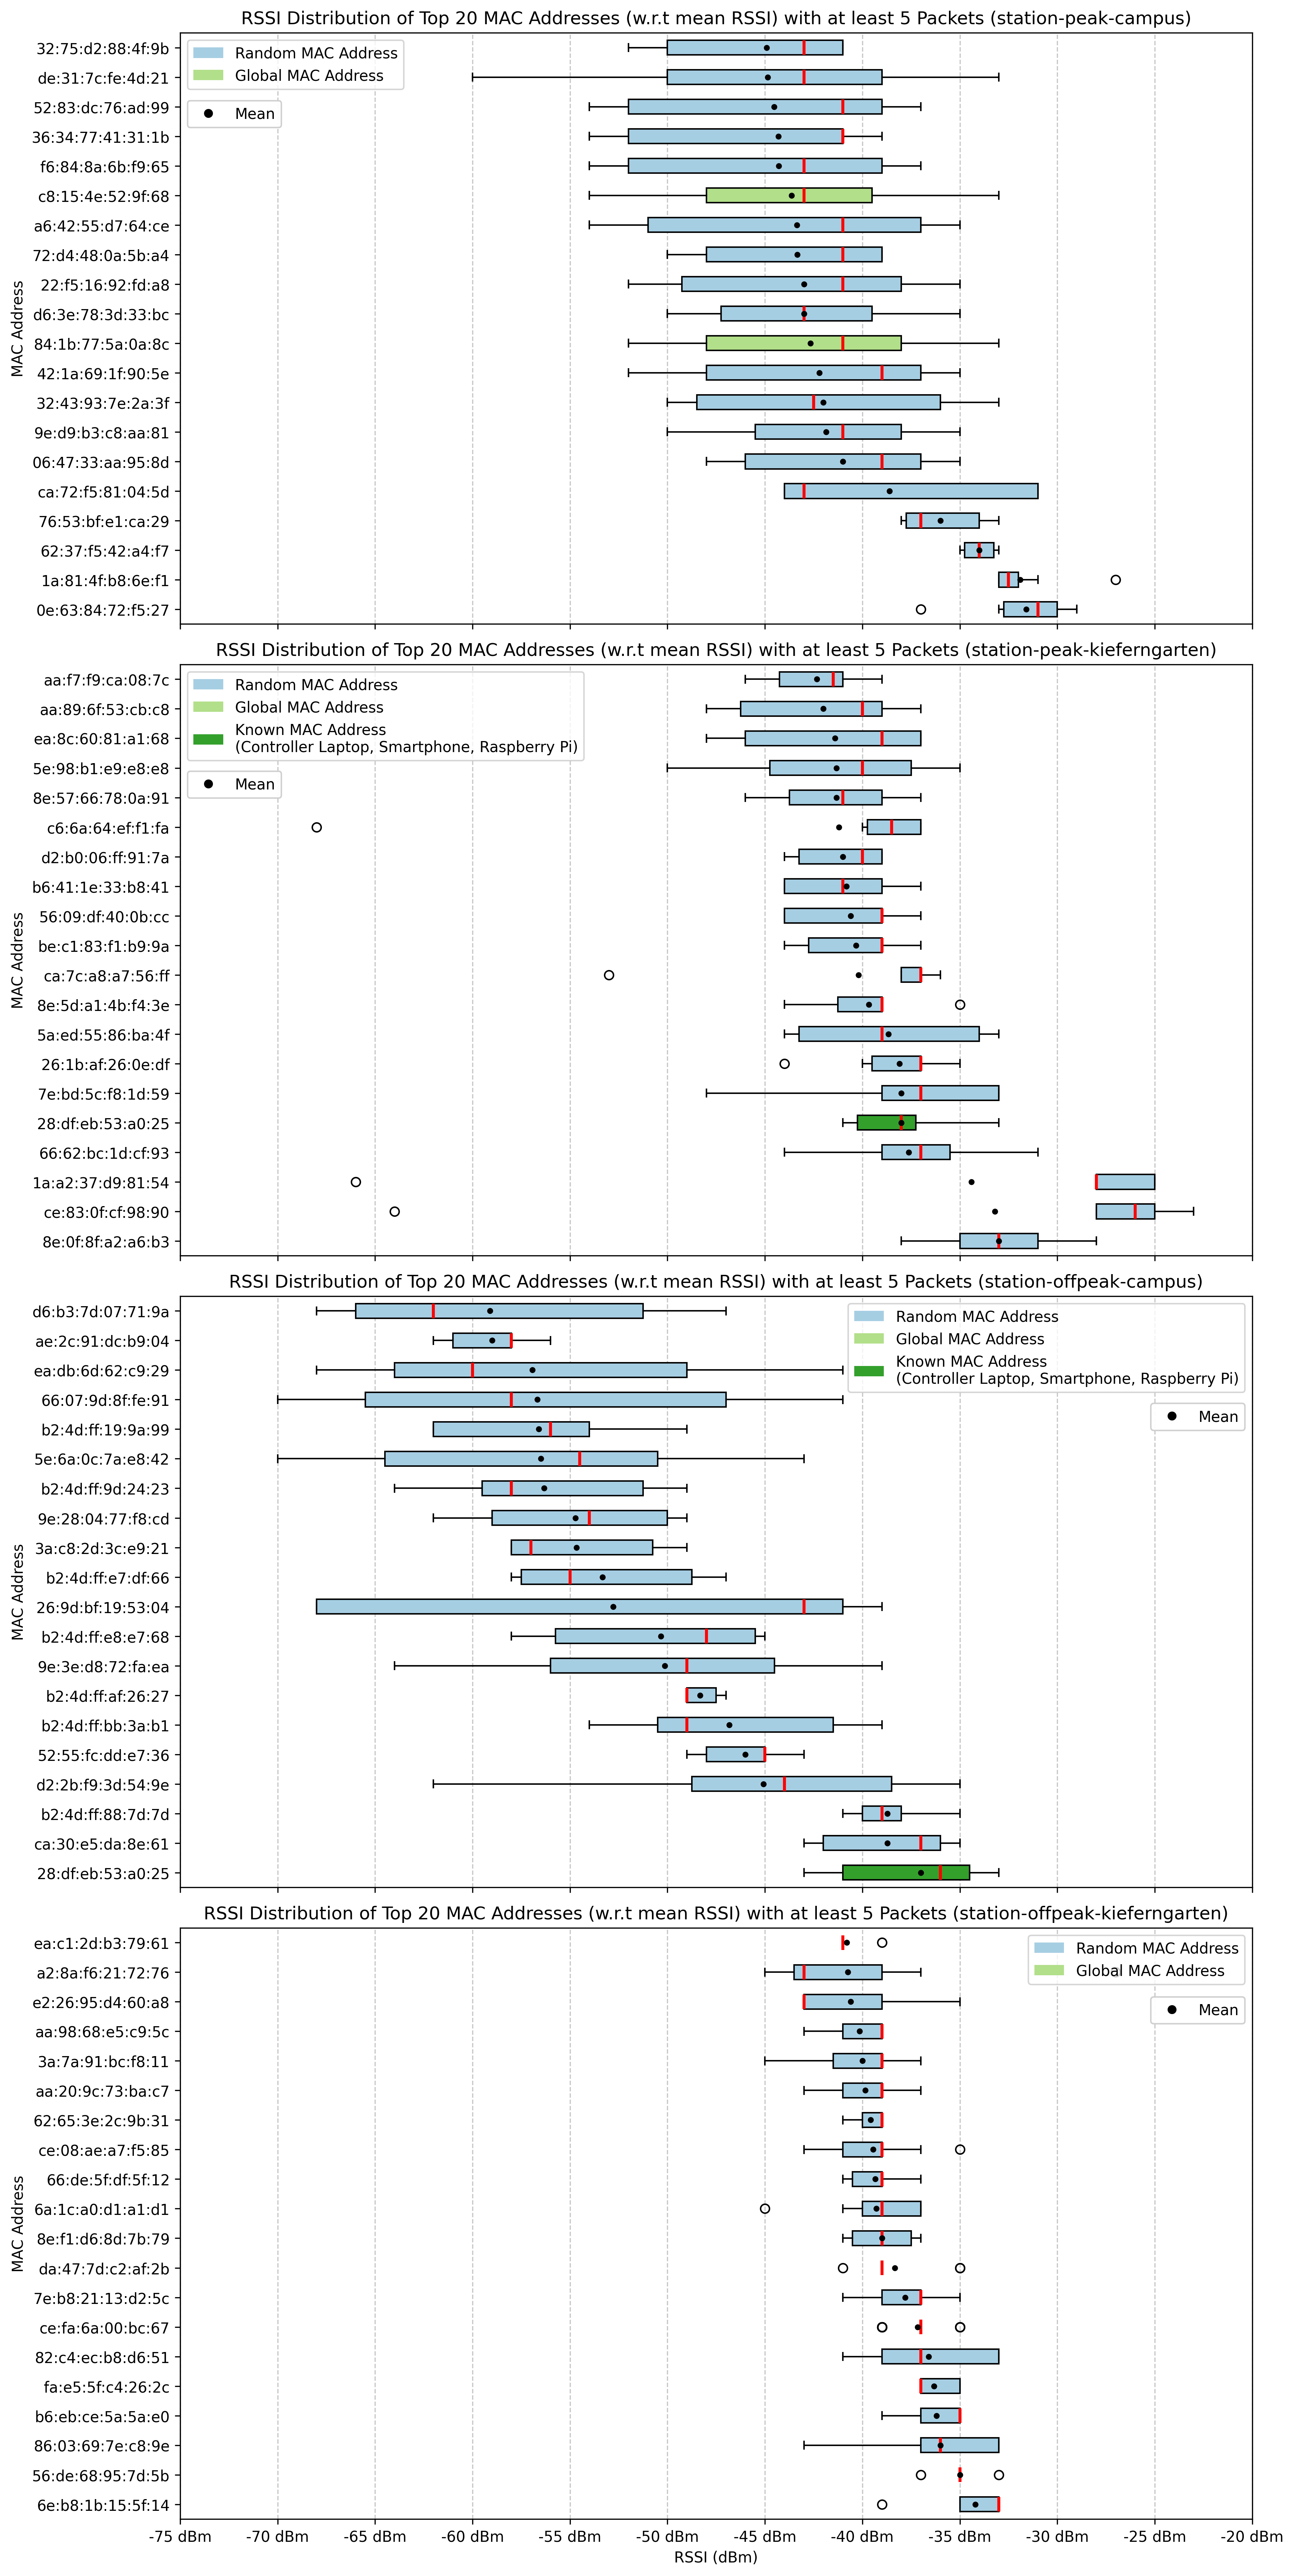
\includegraphics[width=\columnwidth]{images/part1/rssi/top-macs-station-scenarios.png}
    \caption{RSSI Distribution per MAC Address for the Station Scenarios}
    \label{fig:station_rssi_distribution_per_mac}
\end{figure}

Upon closer investigation, we find out that expectedly we have not captured any probe requests from the smartphone and the Raspberry Pi, as the smartphone was on battery saver mode (as described in \cref{sec:part-1/da-co/devices}) therefore was doing passive scanning, and the Raspberry Pi was connected to the smartphone AP, which stopped it from sending probe requests altogether. The controller laptop was connected to the smartphone AP as well, but it was still sending probe requests, which is why we see it in the top 20 MAC addresses in the station-offpeak-campus scenario. The reason why we don't see the controller laptop in the top 20 MAC addresses in the other scenarios is that it sent less than 5 probe requests in those scenarios, which is why it was filtered out.

Unexpectedly, we see that there are many other MAC addresses that have a higher mean RSSI than the devices we used to control the capture process (laptop, smartphone, and Raspberry Pi). This is likely due to the fact that the controller laptop was also on battery saver mode (as described in \cref{sec:part-1/da-co/devices}), which reduced the antenna power of its internal Wi-Fi adapter. Unfortunately, we could not find sufficient documentation on the power behavior of the internal Wi-Fi adapter from the vendor, so the reason for the low RSSI values of the controller laptop remains an open question and requires further testing.

\subsubsection{MAC Address Randomization}
\label{sec:part-1/station/mac-randomization}

We now present the results of the MAC address randomization analysis. We analyze the MAC addresses captured in the station scenarios and check whether they are randomized or not. The results are shown in \cref{tab:mac_randomization_station} and \cref{fig:station_mac_randomization}. The table and the figure show results based on unique MAC addresses, i.e., the same MAC address is counted only once, regardless of how many packets it sent.

\begin{table}[ht]
    \centering
    \caption{MAC Address Randomization Ratios in Station Scenarios}
    \label{tab:mac_randomization_station}
    \resizebox{\columnwidth}{!}{
        \begin{tabular}{|l|r|r|r|r|}
            \hline
            \textbf{Scenario} & \textbf{Random} & \textbf{Global} & \textbf{Total} & \textbf{Random Ratio (\%)} \\
            \hline
            station-peak-campus & 1749 & 39 & 1788 & 97.82\% \\
            station-peak-kieferngarten & 3933 & 26 & 3959 & 99.34\% \\
            station-offpeak-campus & 312 & 6 & 318 & 98.11\% \\
            station-offpeak-kieferngarten & 2031 & 11 & 2042 & 99.46\% \\
            \hline
        \end{tabular}
    }
\end{table}

\begin{figure}
    \centering
    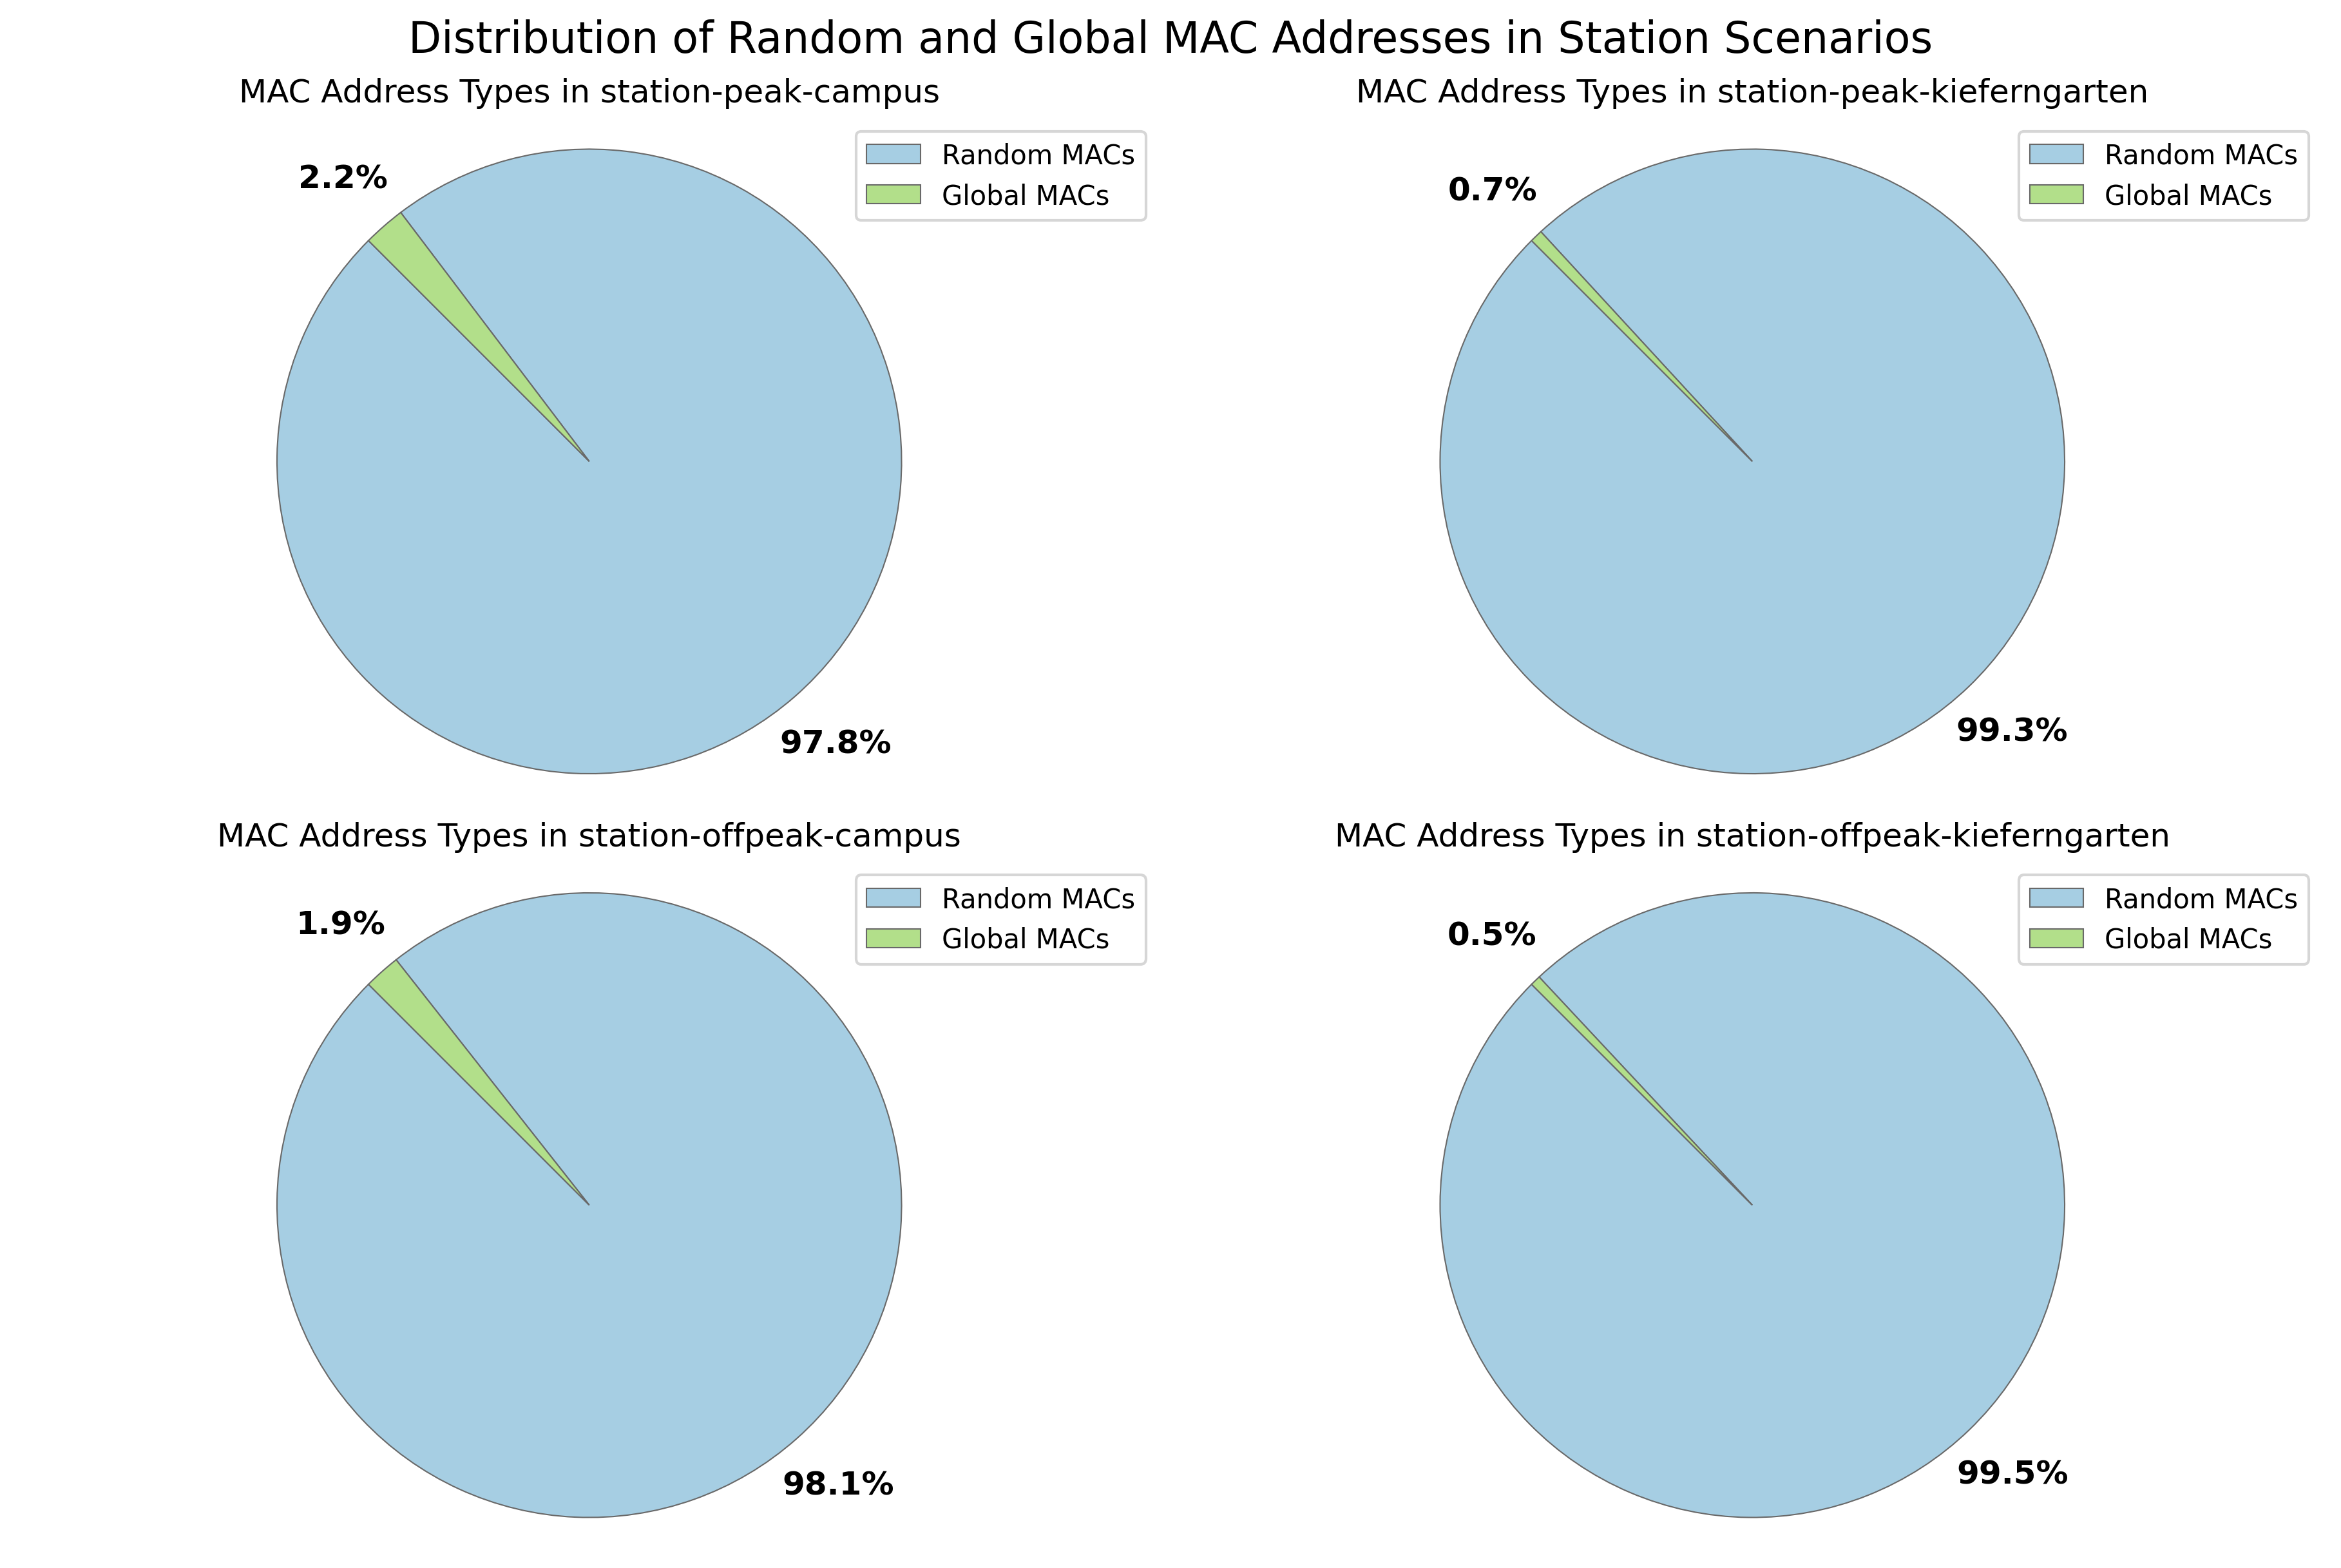
\includegraphics[width=\columnwidth]{images/part1/mac-address-types/station-scenarios.png}
    \caption{MAC Address Randomization for the Station Scenarios}
    \label{fig:station_mac_randomization}
\end{figure}

We did not find any correlation between the crowd size and the ratio of randomized MAC addresses. At first glance, it seems that the Garching Forschungszentrum station has a higher ratio of randomized MAC addresses than the Kieferngarten station. This may be due to the possibility that there are more IoT devices present at the campus (due to it being a research campus), which are less likely to use MAC address randomization. However, this is only a hypothesis and requires further investigation.

\subsubsection{MAC Address Randomization by Packet Count}
\label{sec:part-1/station/mac-randomization-packet-count}

We now turn our attention to the MAC address randomization analysis by packet count. This time we take into account the number of packets sent by each MAC address. The results are shown in \cref{tab:mac_randomization_station_packets} and \cref{fig:station_mac_randomization_packet_count}. The results are based on total packet counts, i.e. the same MAC address is counted as many times as it sent packets.

\begin{table}[ht]
    \centering
    \caption{Packet-based MAC Address Randomization Ratios in Station Scenarios}
    \label{tab:mac_randomization_station_packets}
    \resizebox{\columnwidth}{!}{
    \begin{tabular}{|l|r|r|r|r|}
        \hline
        \textbf{Scenario} & \textbf{Random MAC Pkts} & \textbf{Global MAC Pkts} & \textbf{Total Pkts} & \textbf{Random Pkts Ratio (\%)} \\
        \hline
        station-peak-campus & 6189 & 791 & 6980 & 88.67\% \\
        station-peak-kieferngarten & 11128 & 161 & 11289 & 98.57\% \\
        station-offpeak-campus & 1004 & 91 & 1095 & 91.69\% \\
        station-offpeak-kieferngarten & 4514 & 95 & 4609 & 97.94\% \\
        \hline
    \end{tabular}
    }
\end{table}

\begin{figure}
    \centering
    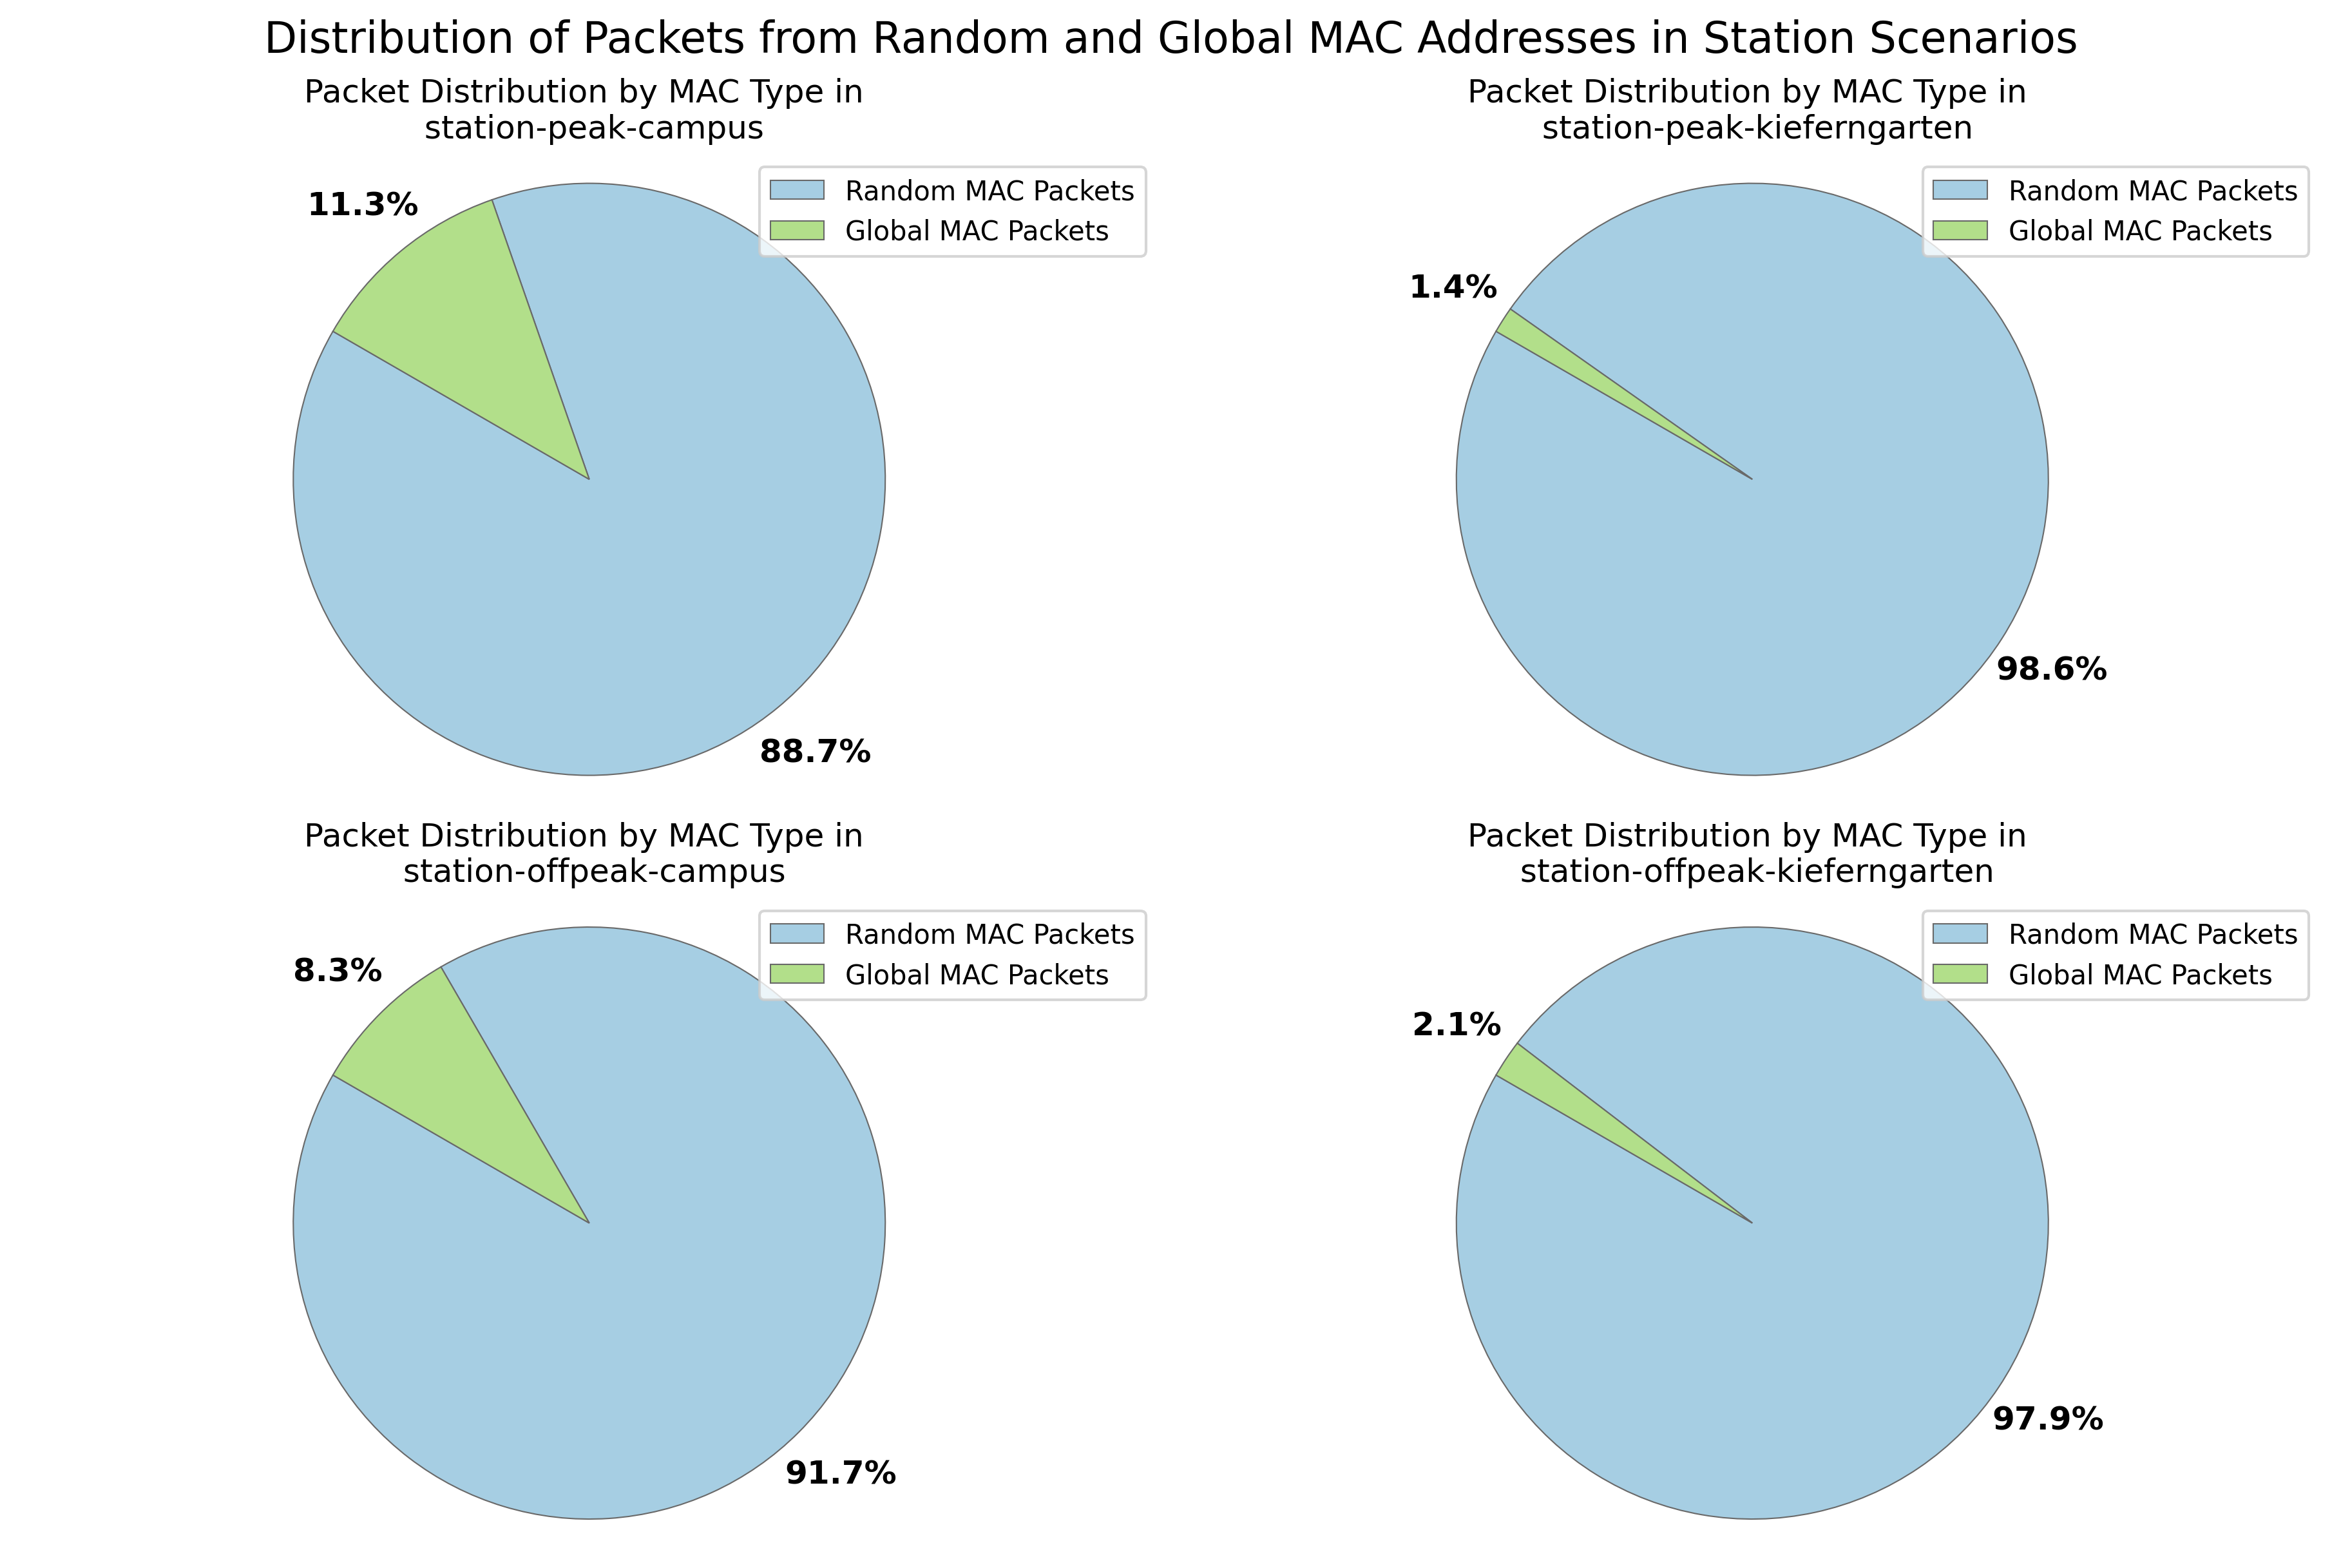
\includegraphics[width=\columnwidth]{images/part1/mac-address-types/station-scenarios-packet-based.png}
    \caption{MAC Address Randomization by Packet Count for the Station Scenarios}
    \label{fig:station_mac_randomization_packet_count}
\end{figure}

\subsubsection{Vendor OUIs}
\label{sec:part-1/station/oui}

We present the top 10 most common vendor OUIs in the station scenarios by unique MAC address count. The results are shown in \cref{tab:station_oui}. Just like in the MAC randomization analysis, we only take into account unique MAC addresses, i.e., the same OUI is counted only once, regardless of how many packets it sent.

\begin{figure}
    \centering
    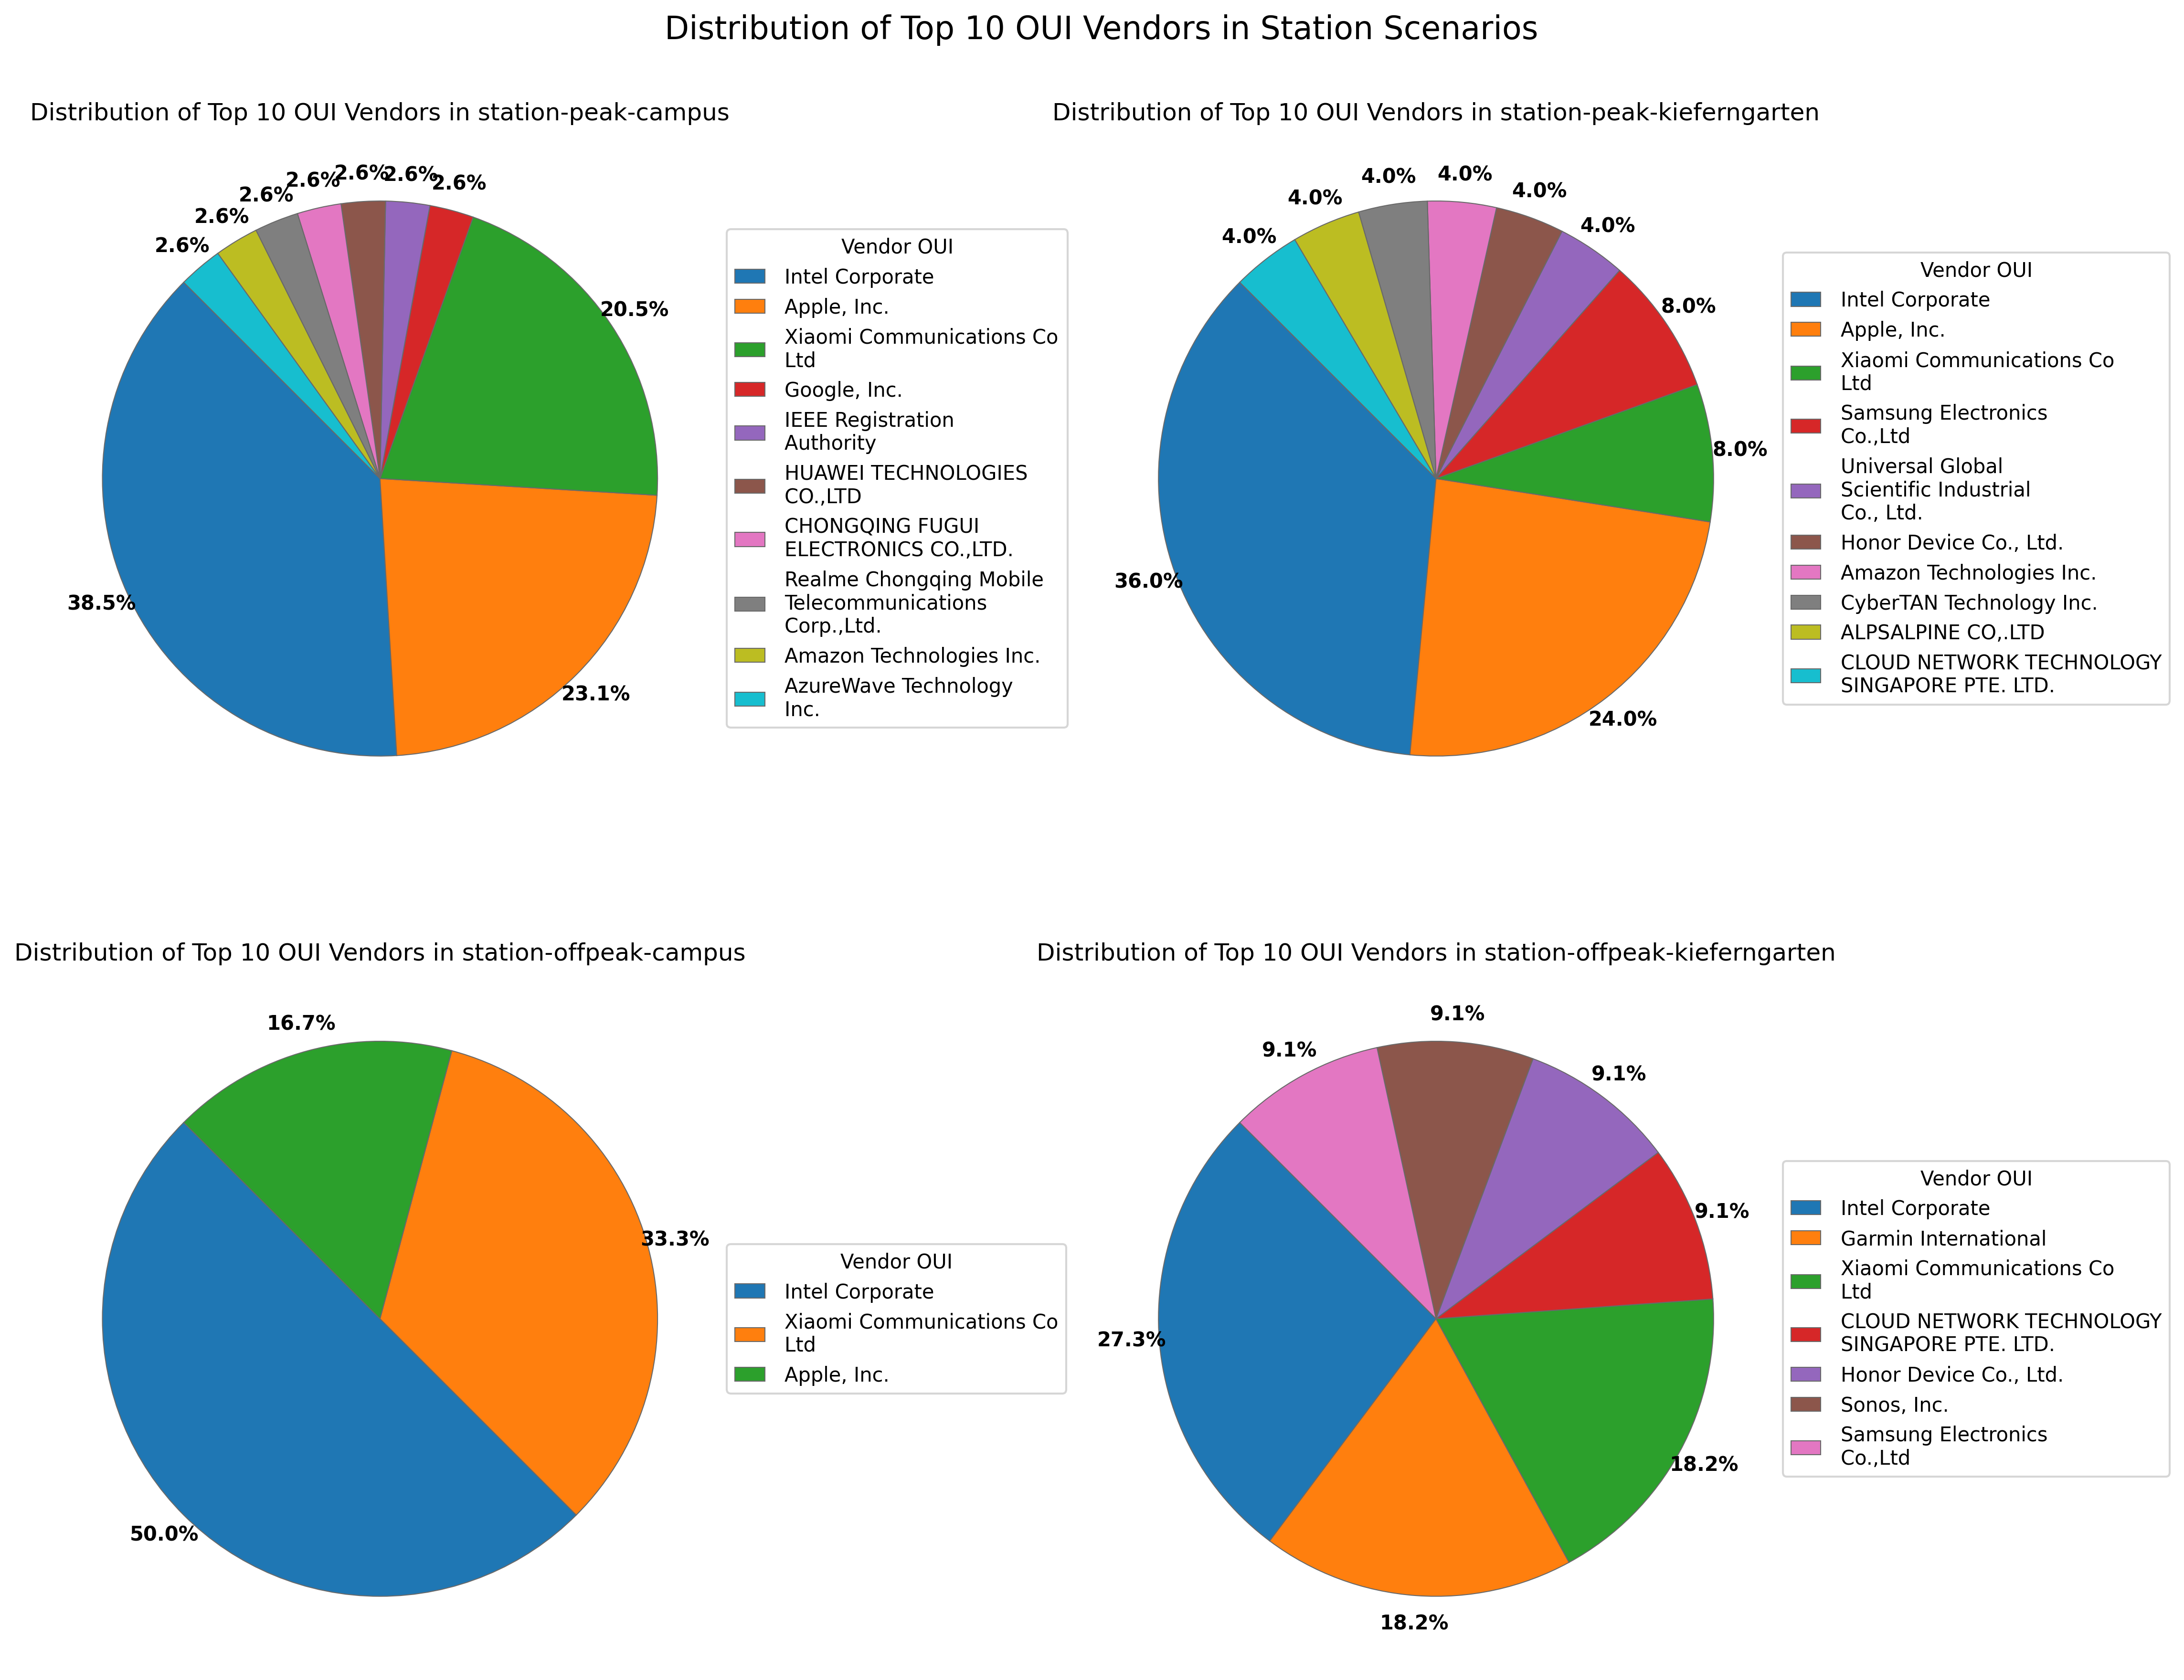
\includegraphics[width=\columnwidth]{images/part1/oui-vendors/station-scenarios.png}
    \caption{Top 10 Vendor OUIs in the Station Scenarios}
    \label{tab:station_oui}
\end{figure}

We can clearly see that the OUIs are more varied in the peak scenarios than in the off-peak scenarios. This is because more devices mean it is more likely to have a wider variety of devices present.

\subsubsection{Vendor OUIs by Packet Count}
\label{sec:part-1/station/oui-packet-count}

We now turn our attention to the vendor OUIs by packet count. The results are shown in \cref{tab:station_oui_packet_count}. The results are based on total packet counts, i.e. the same OUI is counted as many times as it sent packets.

\begin{figure}
    \centering
    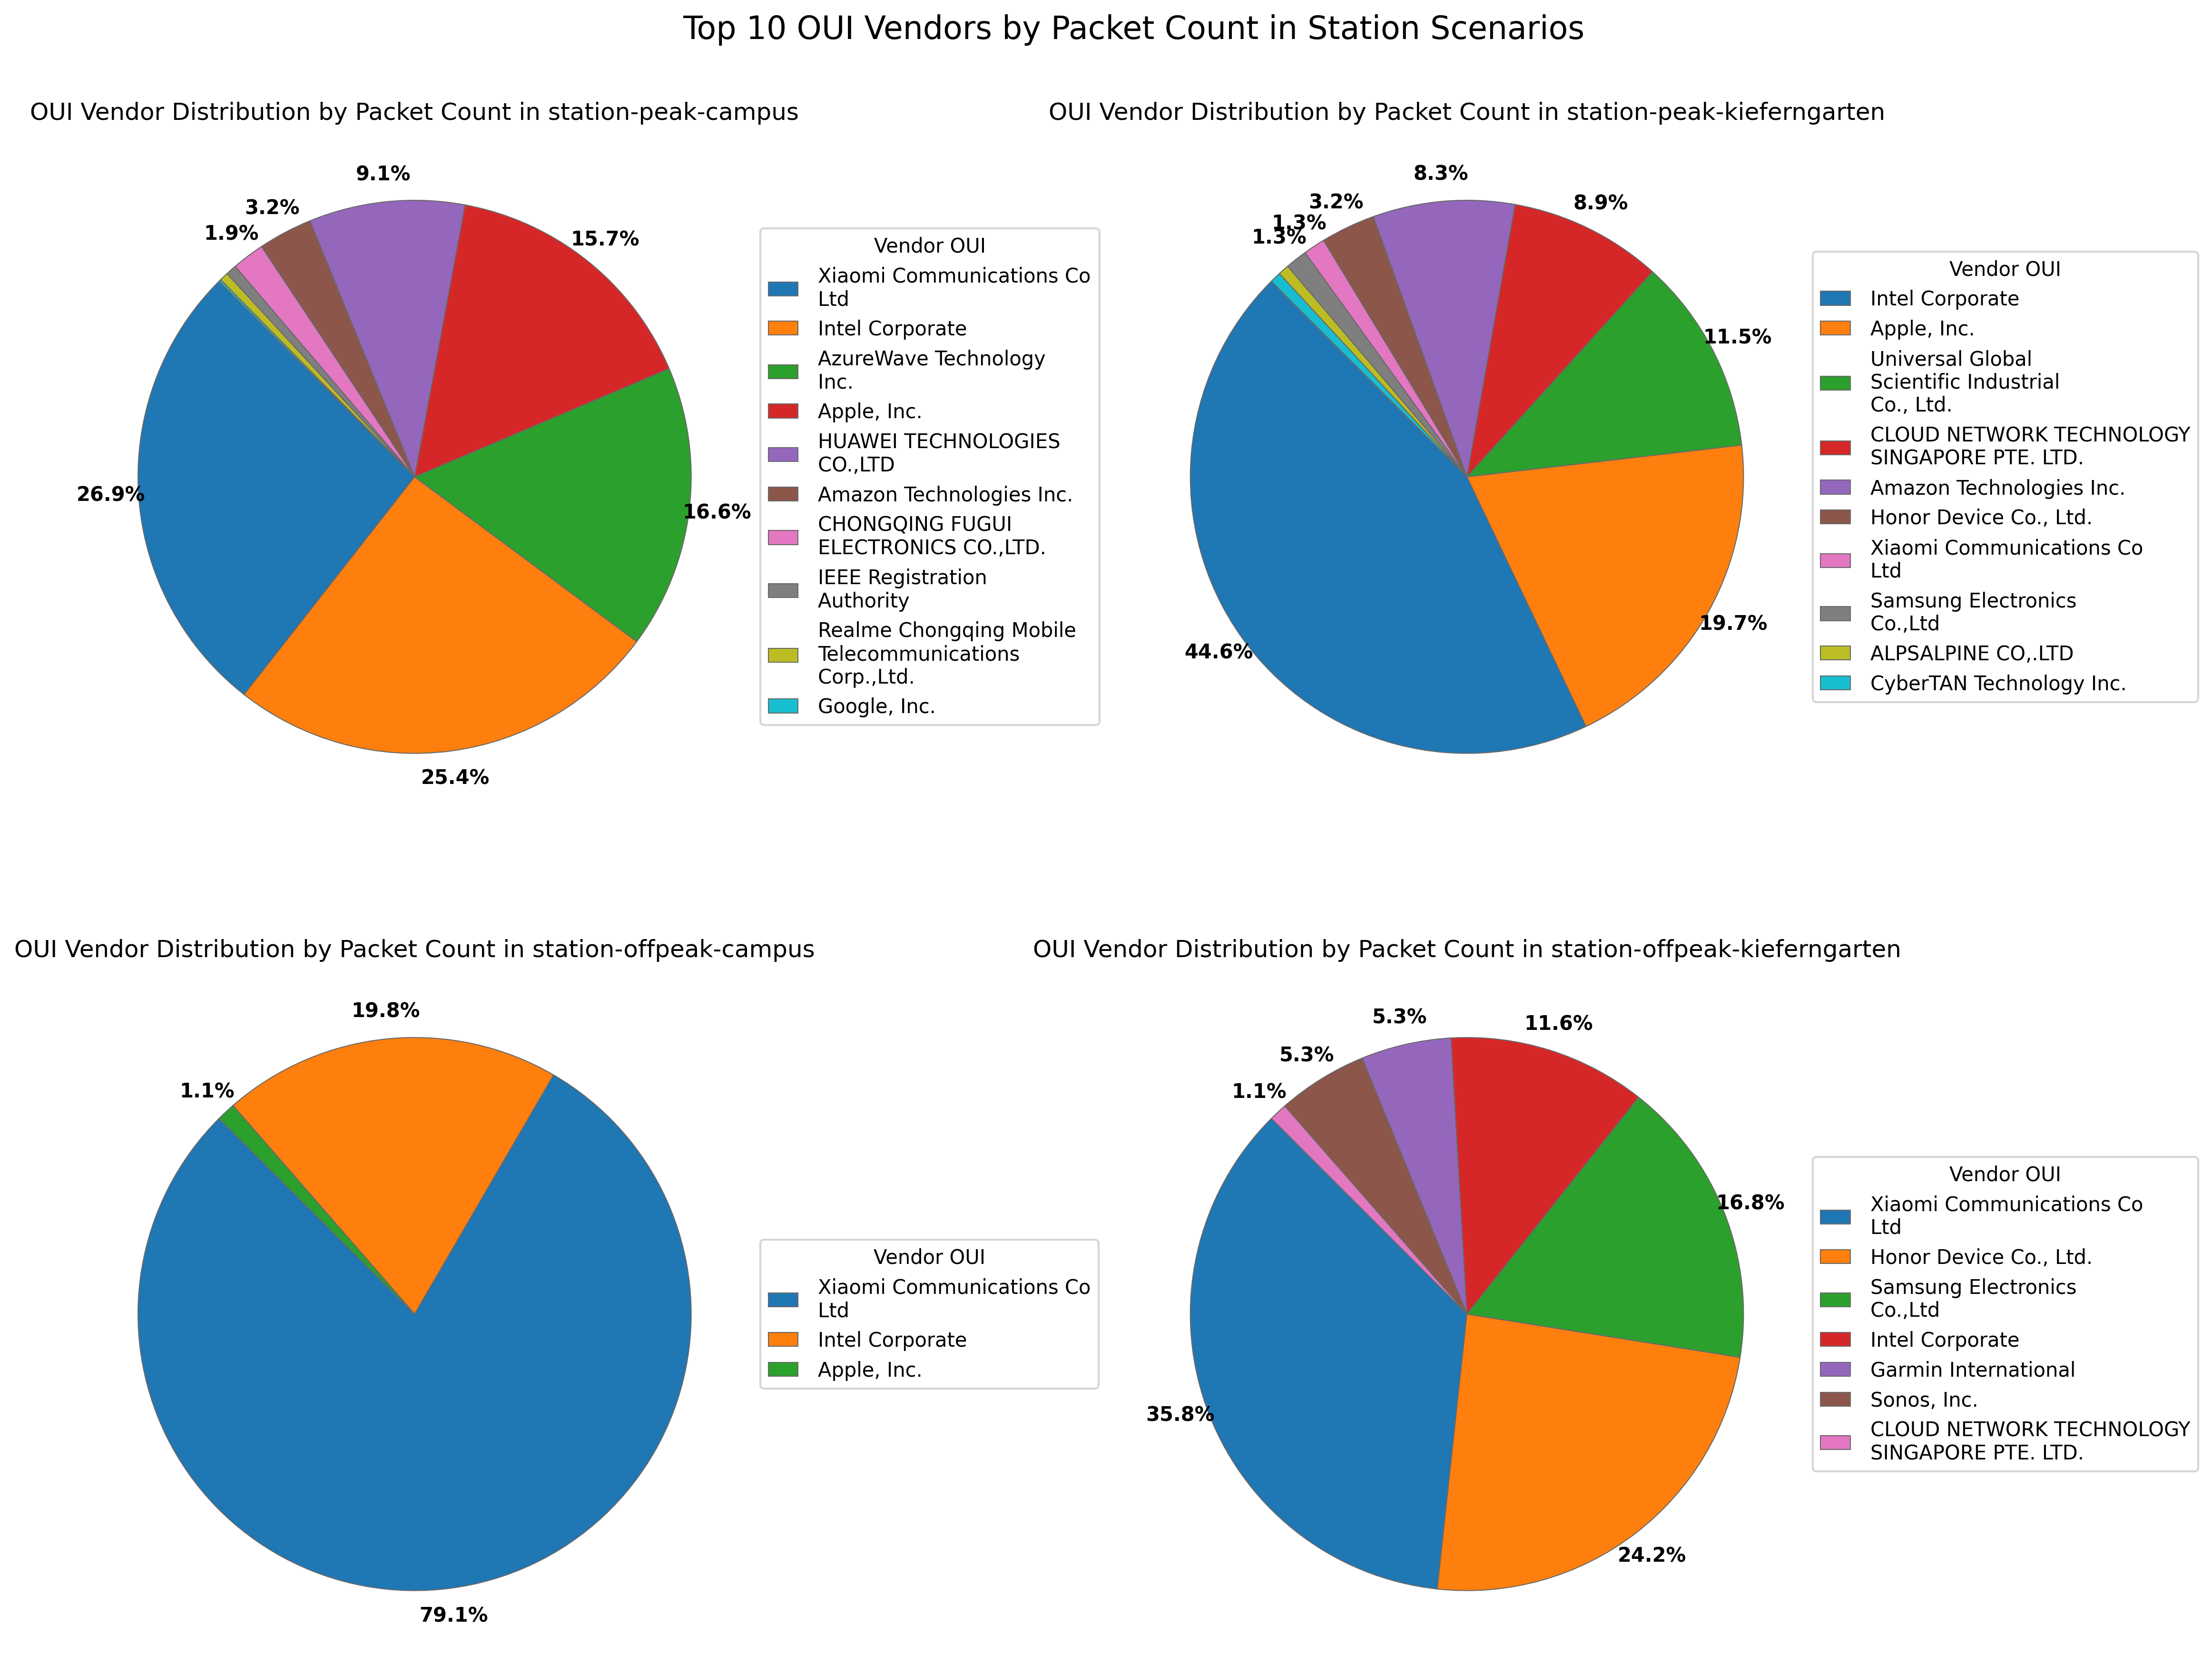
\includegraphics[width=\columnwidth]{images/part1/oui-vendors/station-scenarios-packet-count.png}
    \caption{Top 10 Vendor OUIs by Packet Count in the Station Scenarios}
    \label{tab:station_oui_packet_count}
\end{figure}

Combined with the results of the previous section, we see that some devices from certain vendors send probe requests more frequently than others. For example, in the station-offpeak-campus scenario, we see that Xiaomi devices make up 33.3\% of the unique MAC addresses, but they make up 79.1\% of the total packet counts. Therefore, they send probe requests more frequently compared to other vendors in this scenario. The results in this section, combined with the results in the previous section, allow us to compare the average probe request frequency behavior of different vendors, which is an interesting topic for further analysis. It is worth noting that the arrival times of these devices in the environment greatly affect the shares; for a stronger conclusion, different experiments should be conducted.

\subsubsection{SSIDs}
\label{sec:part-1/station/ssids}

Finally, we present the SSID distribution of the probe requests captured in the station scenarios. We present the number of SSID set vs SSID not set packets and their ratios in the station scenarios in \cref{tab:ssid_presence_station} and \cref{fig:ssid_presence_station} respectively. We then finalize the section with the list of the top 10 most common SSIDs in the station scenarios in \cref{tab:station_ssids}.

\begin{table}[ht]
    \centering
    \caption{Packet Distribution by SSID Presence in Station Scenarios}
    \label{tab:ssid_presence_station}
    \resizebox{\columnwidth}{!}{
    \begin{tabular}{|l|r|r|r|r|}
        \hline
        \textbf{Scenario} & \textbf{SSID Set} & \textbf{SSID Not Set} & \textbf{Total Packets} & \textbf{SSID Set Ratio (\%)} \\
        \hline
        station-peak-campus & 2678 & 4302 & 6980 & 38.37\% \\
        station-peak-kieferngarten & 1806 & 9483 & 11289 & 16.00\% \\
        station-offpeak-campus & 472 & 623 & 1095 & 43.11\% \\
        station-offpeak-kieferngarten & 633 & 3976 & 4609 & 13.73\% \\
        \hline
    \end{tabular}
    }
\end{table}

\begin{figure}
    \centering
    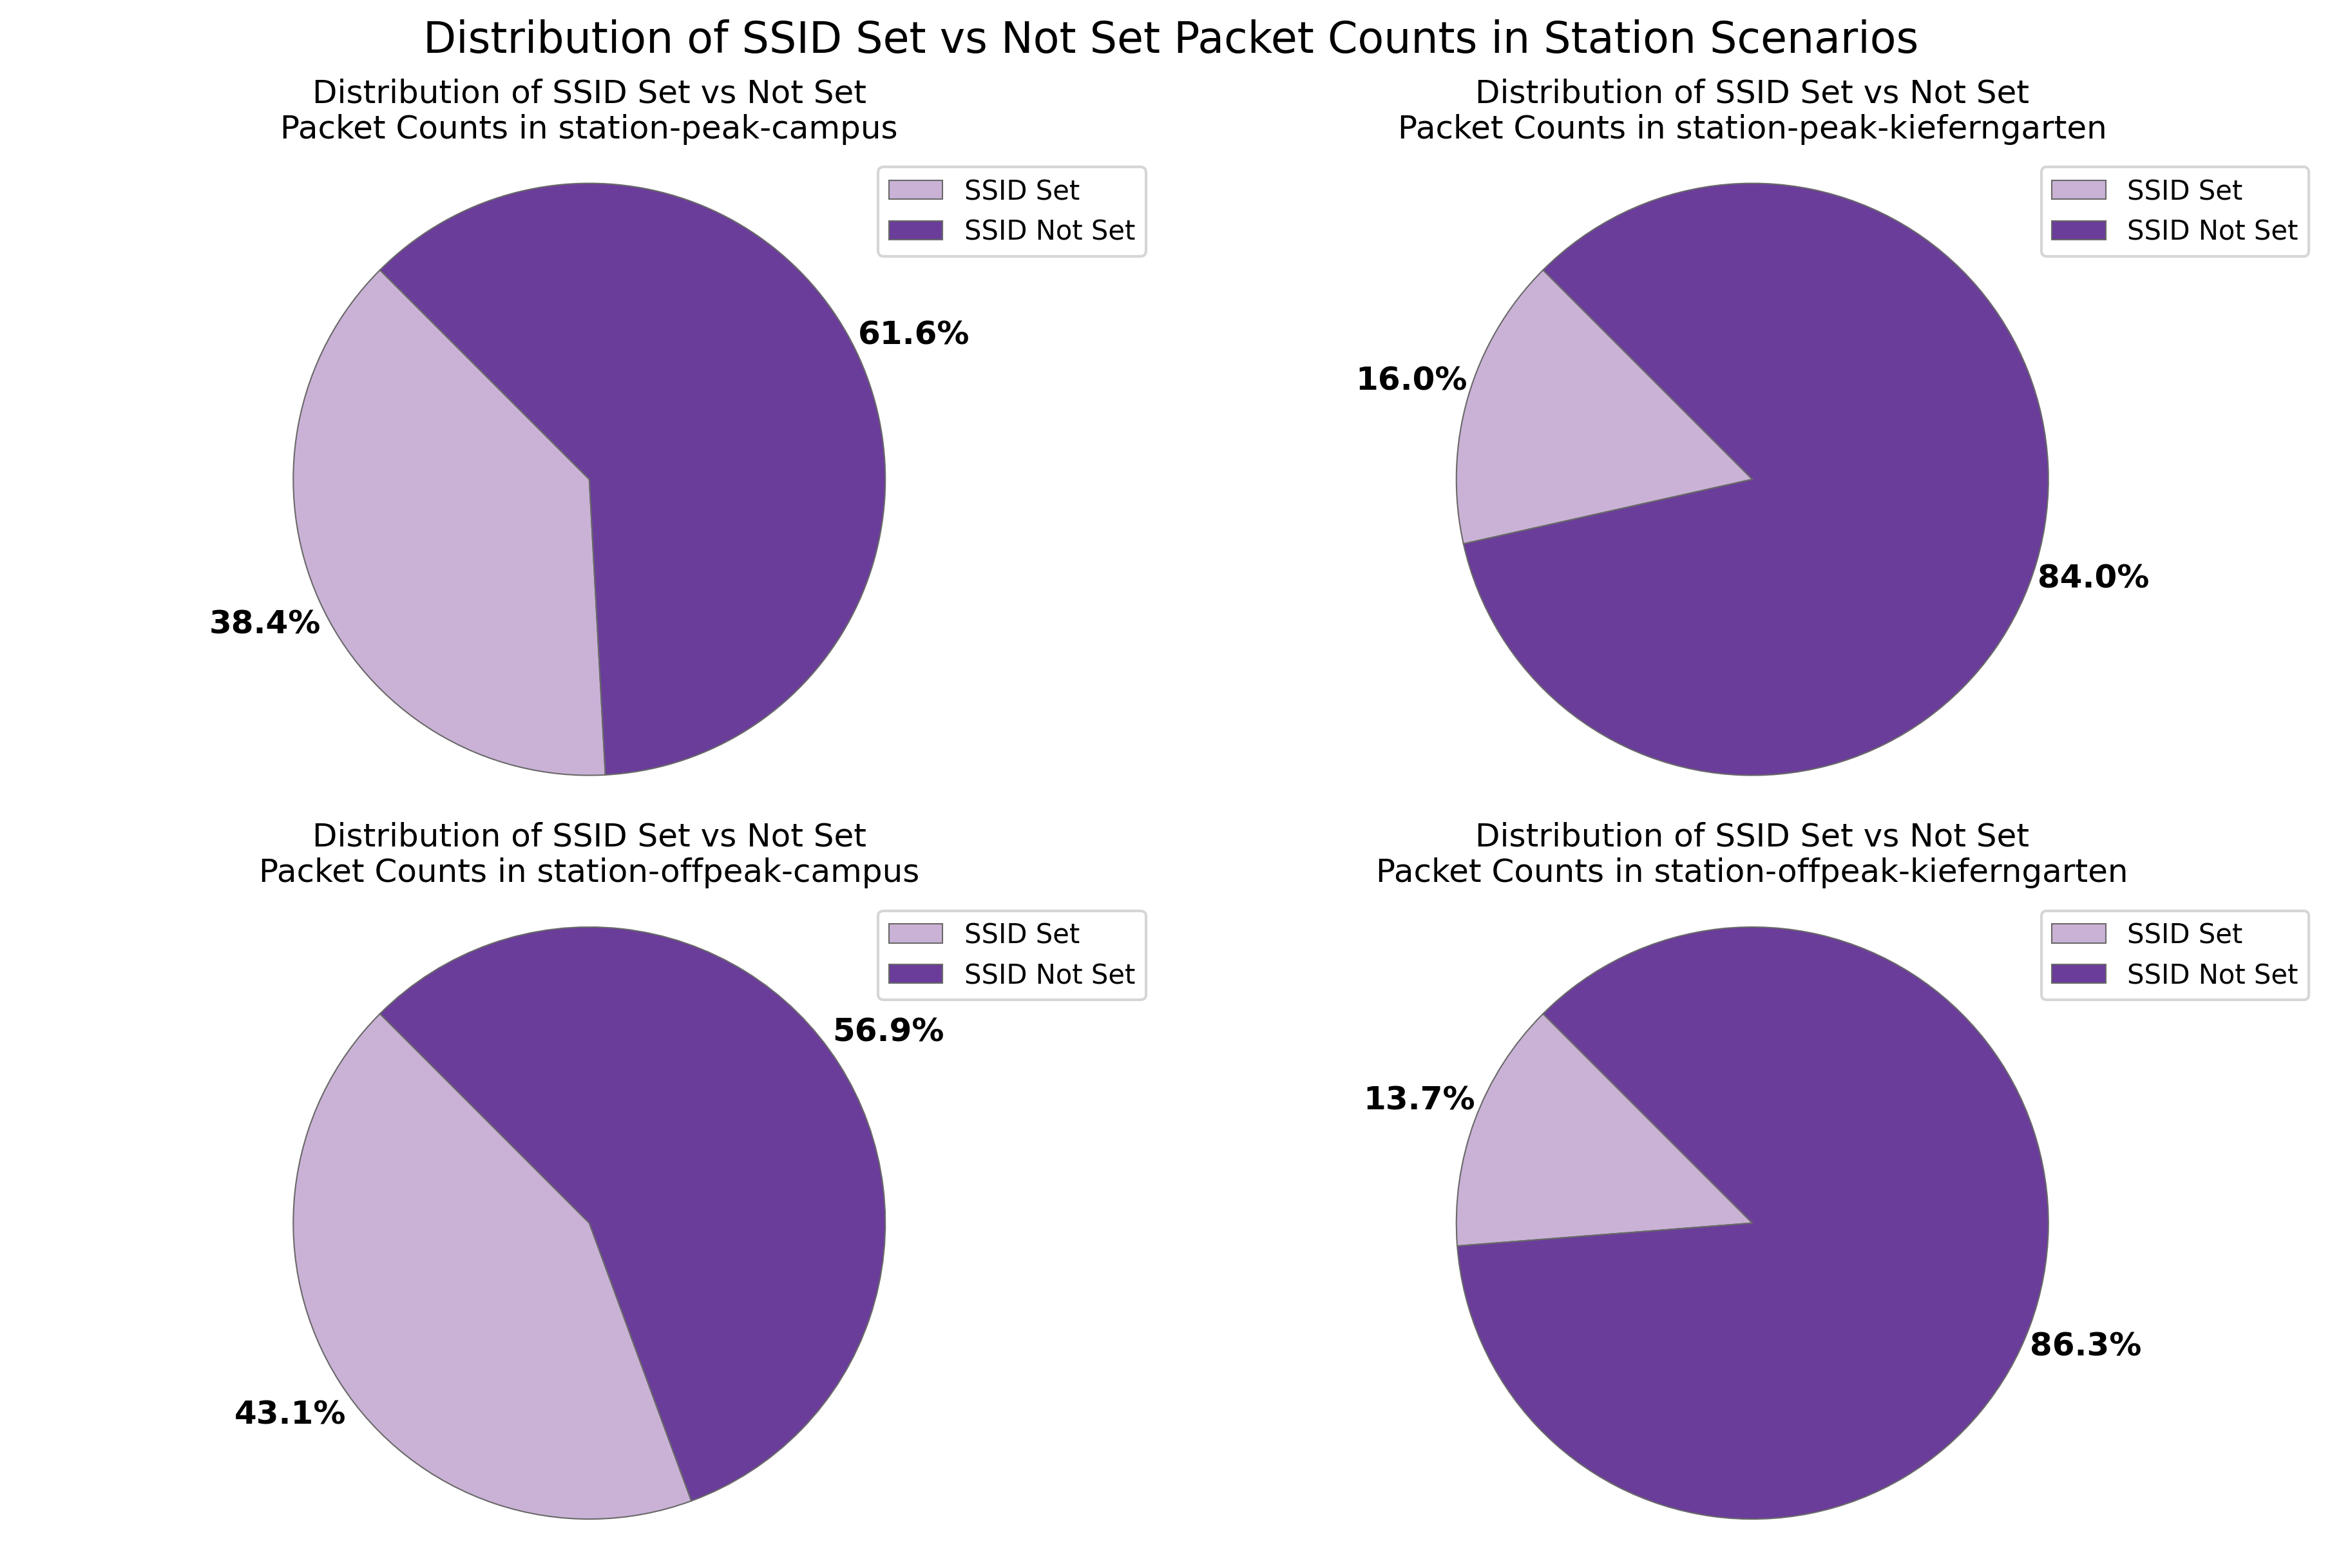
\includegraphics[width=\columnwidth]{images/part1/ssid/station-scenarios.png}
    \caption{SSID Presence in the Station Scenarios}
    \label{fig:ssid_presence_station}
\end{figure}

\begin{figure}
    \centering
    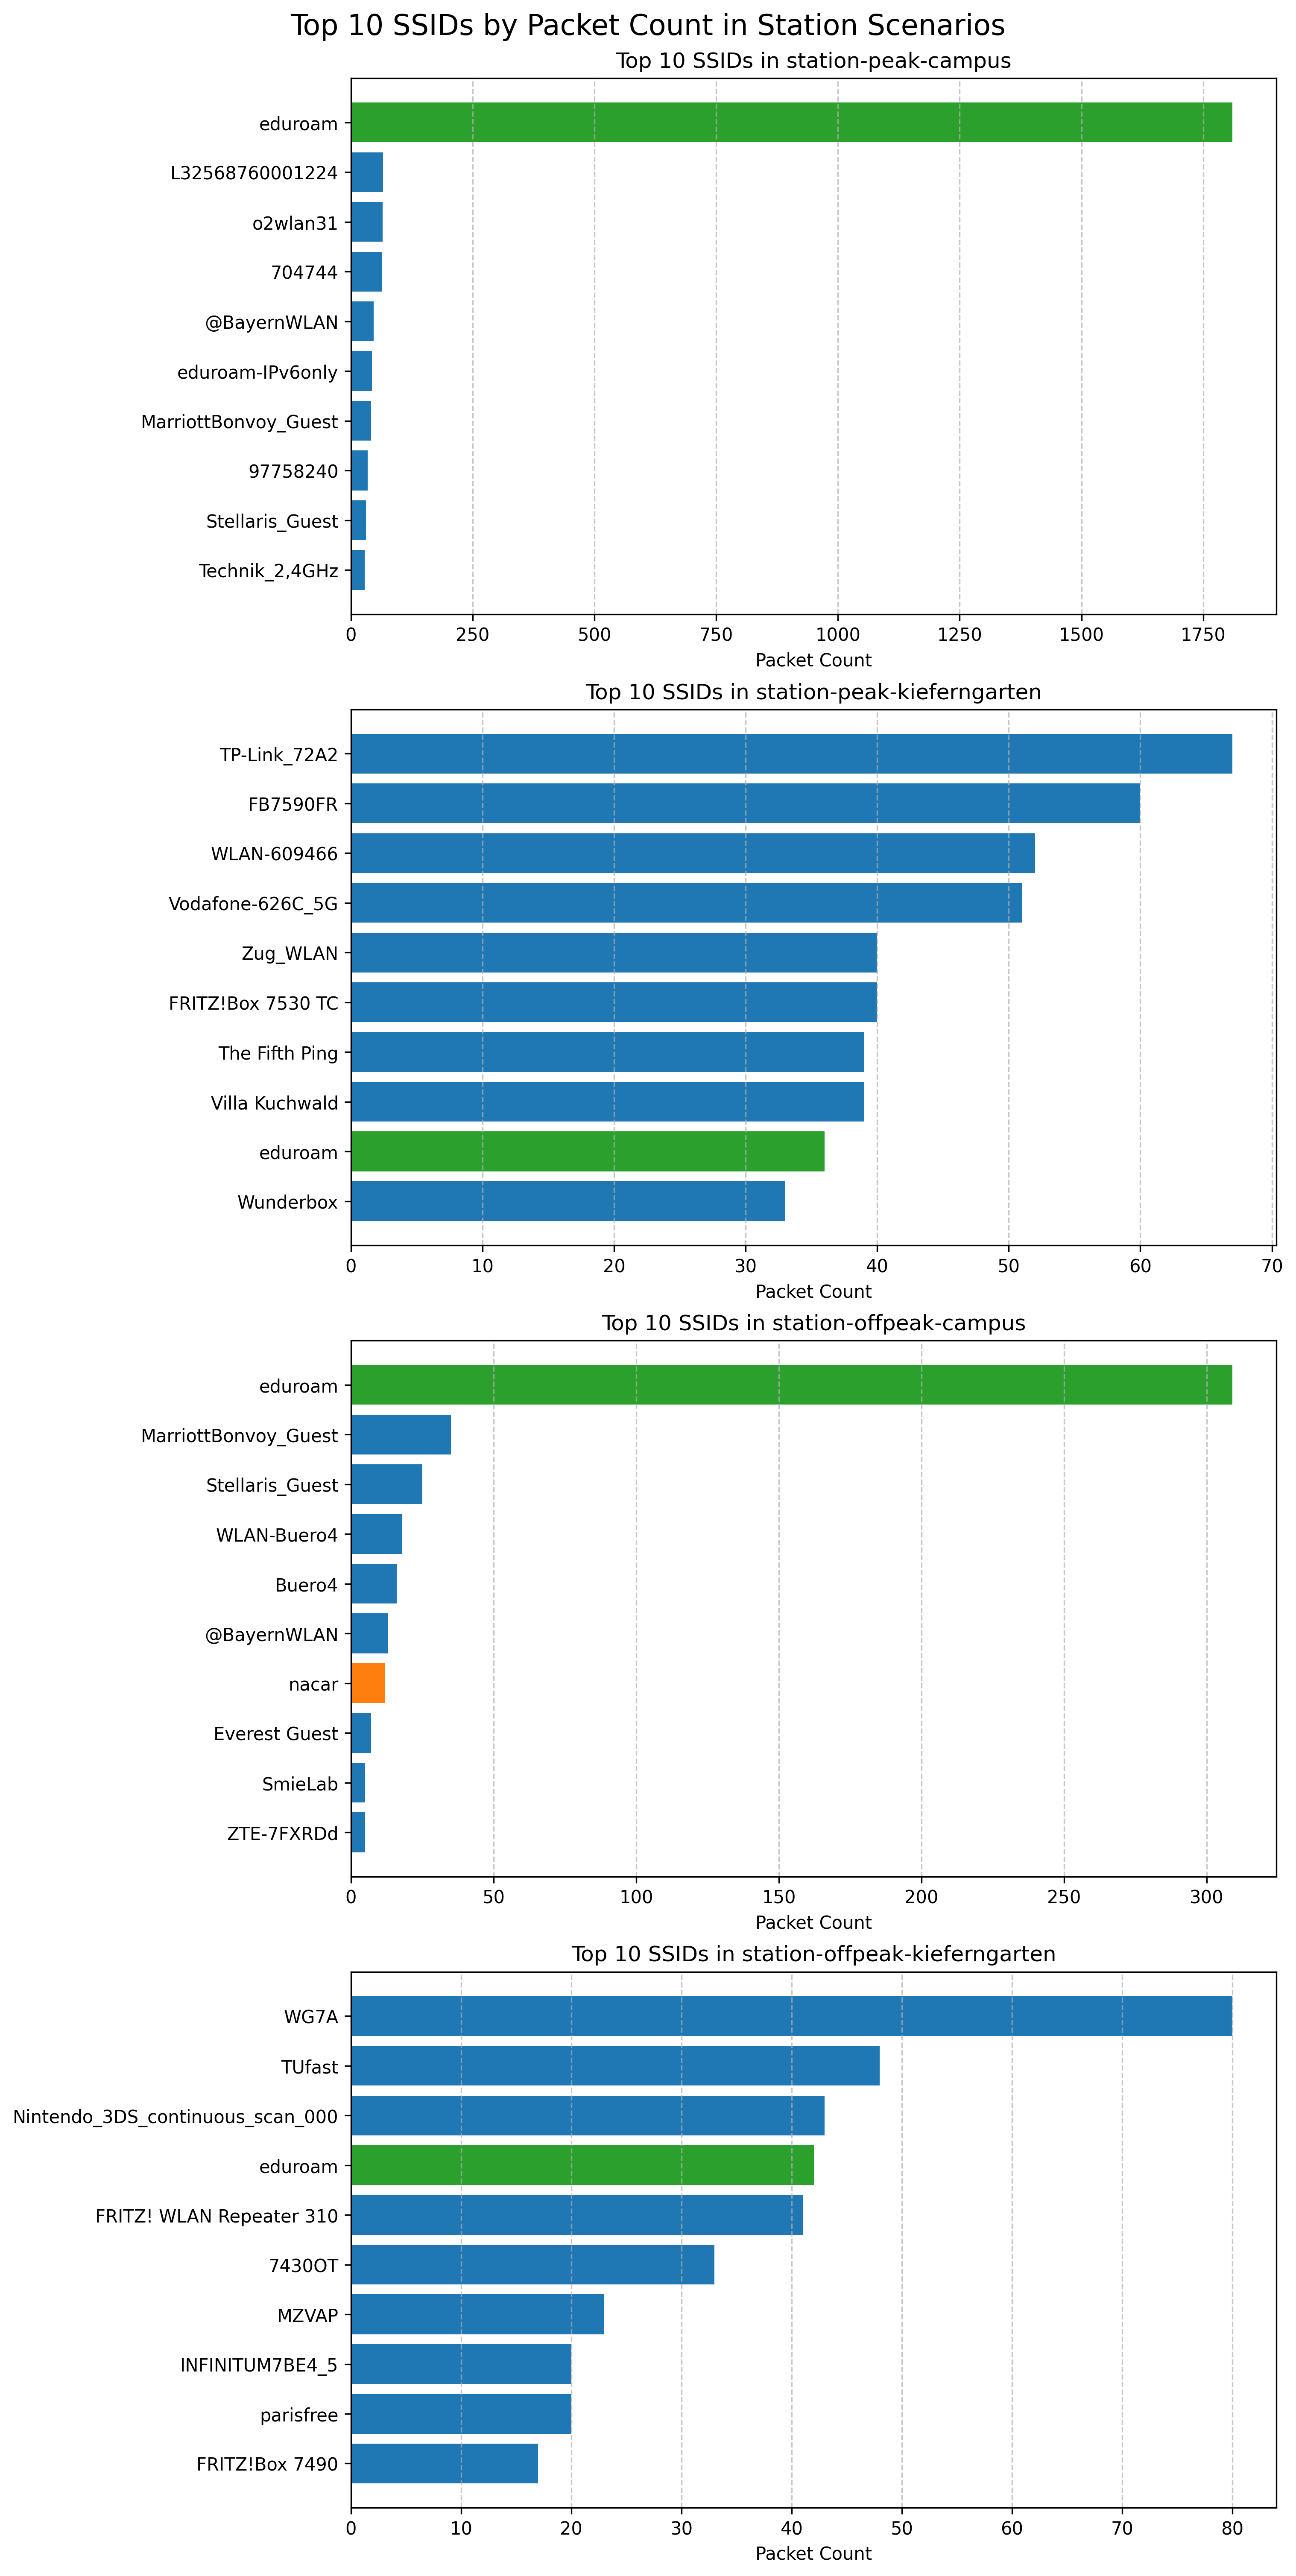
\includegraphics[width=\columnwidth]{images/part1/ssid/top-ssids-station-scenarios.png}
    \caption{Top 10 SSIDs in the Station Scenarios}
    \label{tab:station_ssids}
\end{figure}

We can see that expectedly, probe requests that are looking for SSID "eduroam" are the most common in the station scenarios overall, especially in the Garching Forschungszentrum station, as it is the campus station. We can also see the SSID "nacar", which is the SSID of the smartphone AP, and all the probe requests sent looking for it are sent by the controller laptop.

\subsection{Results - Train Scenarios}
\label{sec:part-1/res-train}

\subsubsection{Crowd Estimations}
\label{sec:part-1/train/crowd-estimations}

Like before, the crowd estimations are done visually during the captures. 

For the crowd estimations of the trains, the number of people in the current train car is counted, and then multiplied by 6 (the number of cars in a train).

\begin{figure}
    \centering
    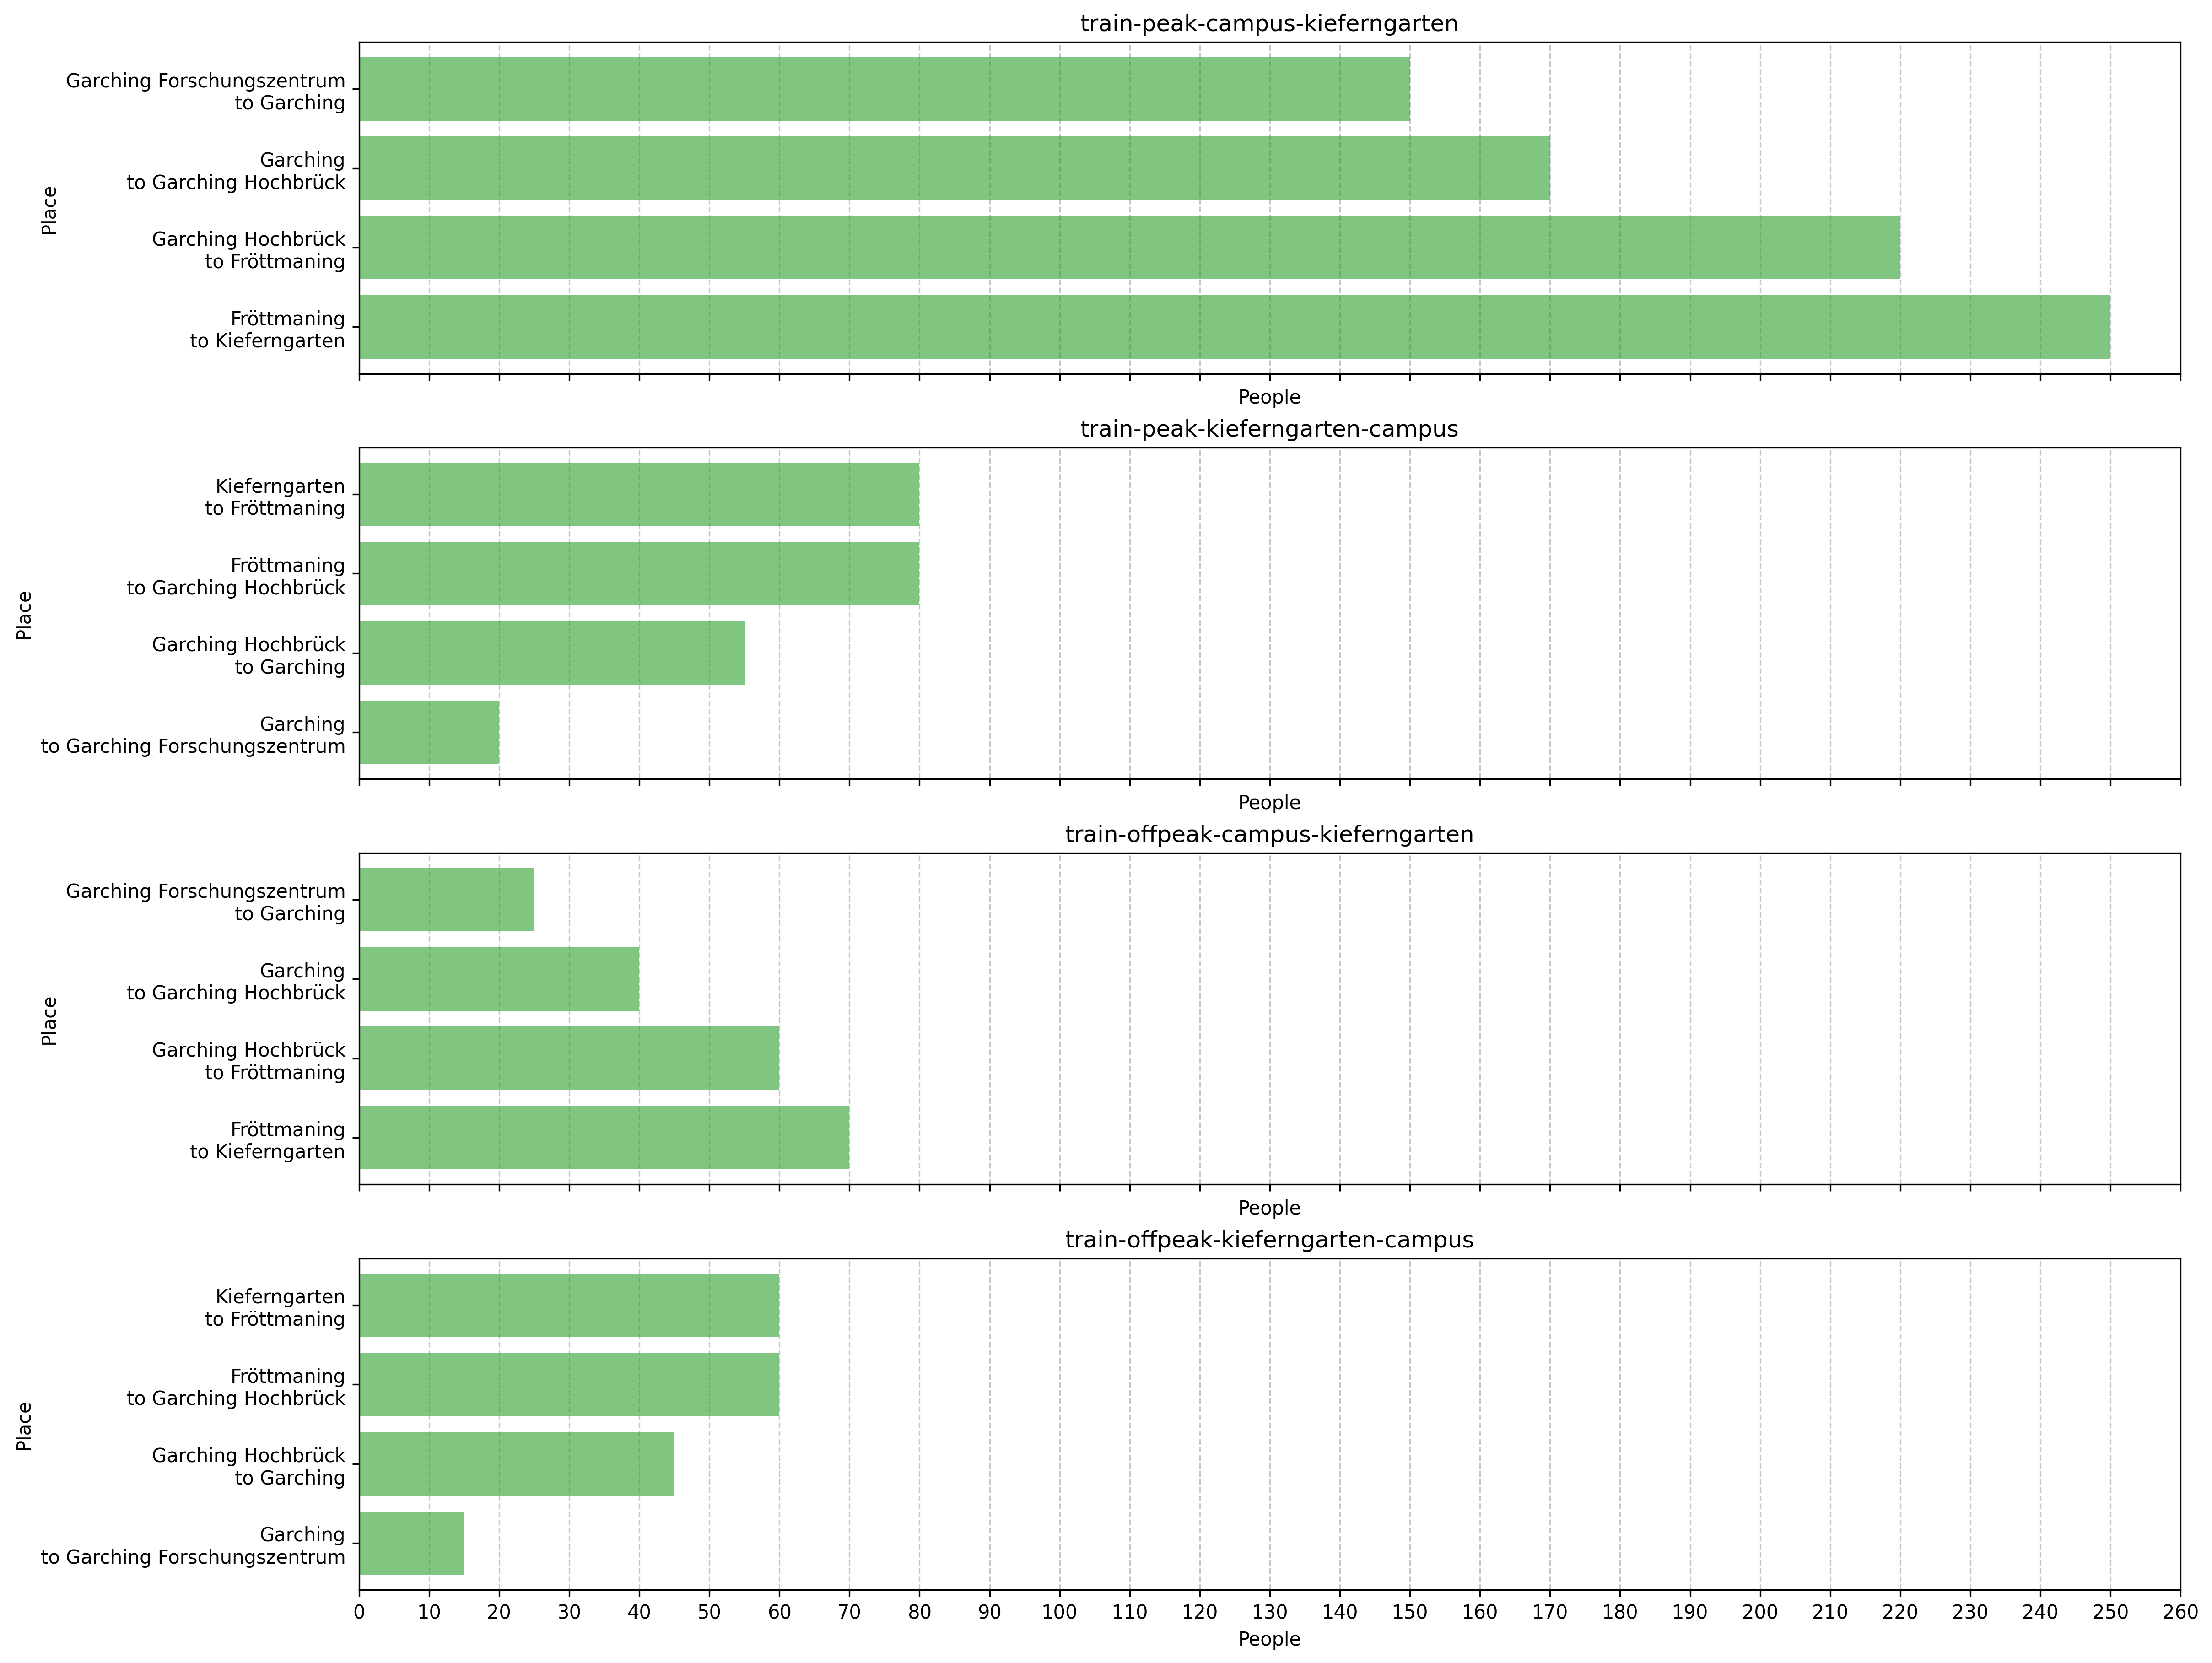
\includegraphics[width=\columnwidth]{images/part1/crowd-estimations/crowd-estimate-trains.png}
    \caption{Crowd Estimations for the Train Scenarios}
    \label{tab:crowd_estimate-trains}
\end{figure}

\subsubsection{Packet Counts}
\label{sec:part-1/train/packet-counts}

The cumulative packet counts and the packet arrival rates are shown in \cref{fig:train_cumulative_packet_counts} and \cref{fig:train_packet_arrival_rate}, respectively. Just like with the station scenarios, the cumulative packet counts show the total number of packets captured over time, while the packet arrival rates show the number of packets captured per 5 seconds with the smoothing described in \cref{sec:part-1/ana/noise-filtering}.

\begin{figure}
    \centering
    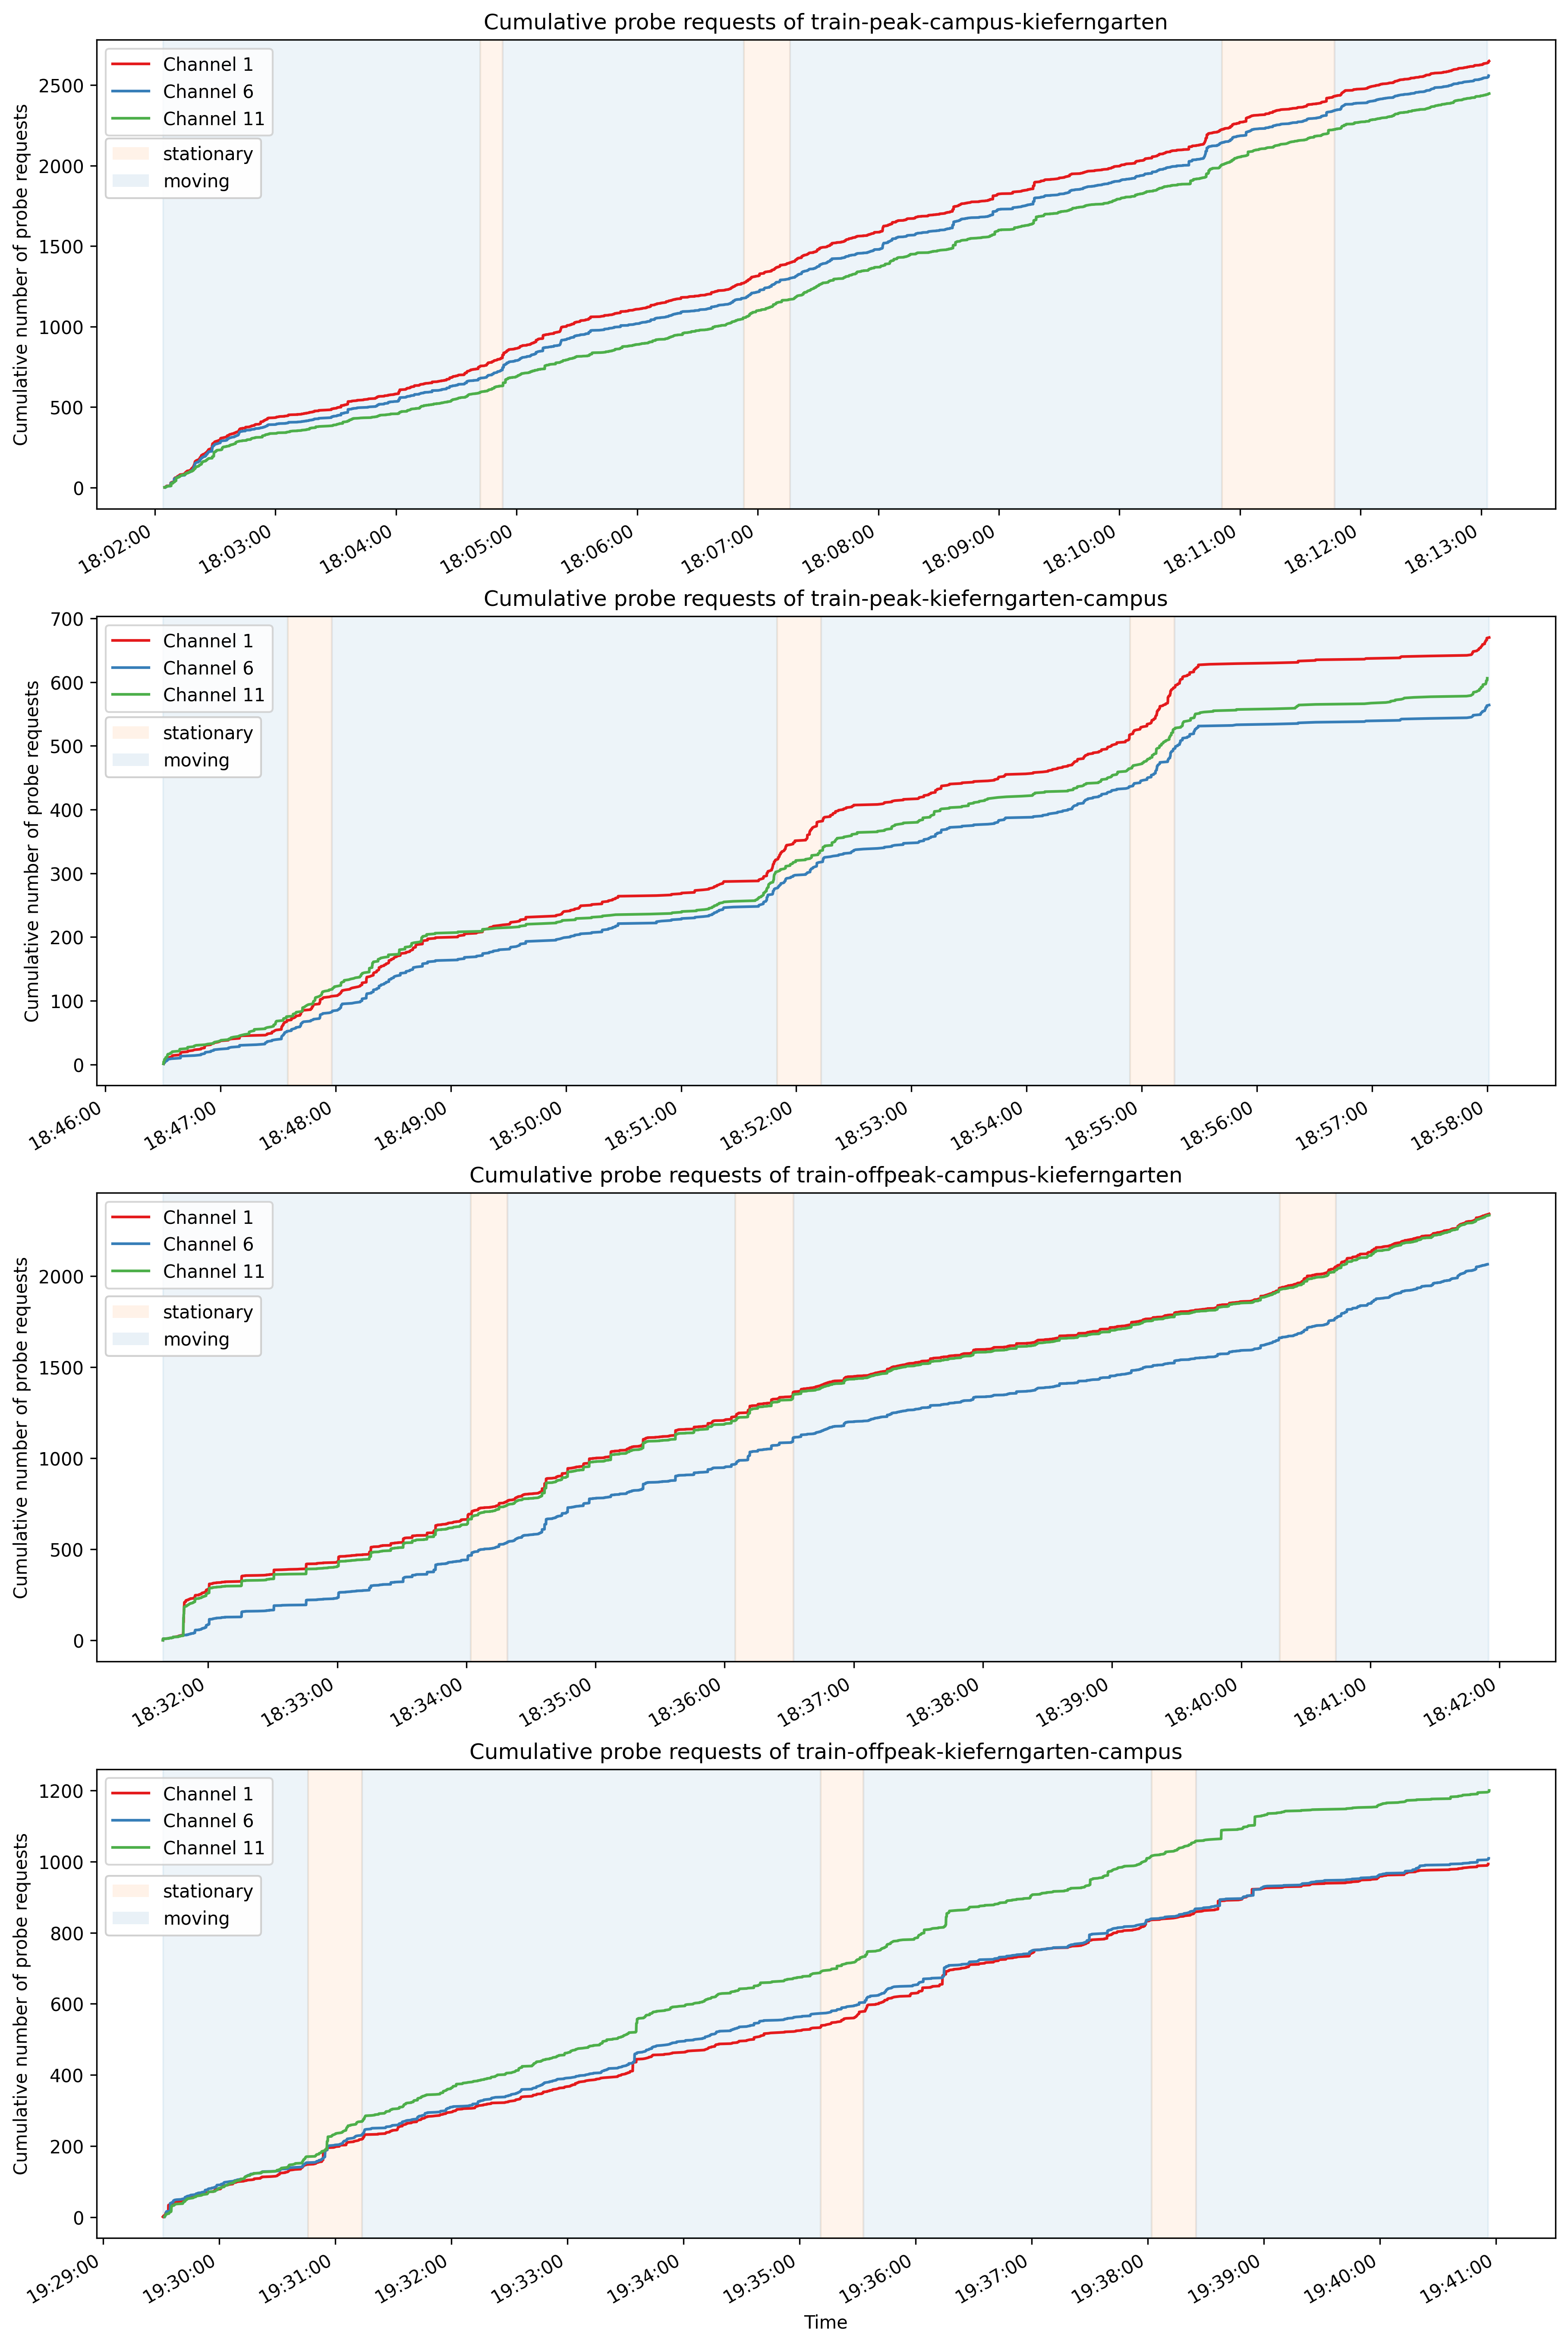
\includegraphics[width=\columnwidth]{images/part1/cumulative-packet-counts/train-scenarios.png}
    \caption{Cumulative Packet Counts for the Train Scenarios}
    \label{fig:train_cumulative_packet_counts}
\end{figure}

\begin{figure}
    \centering
    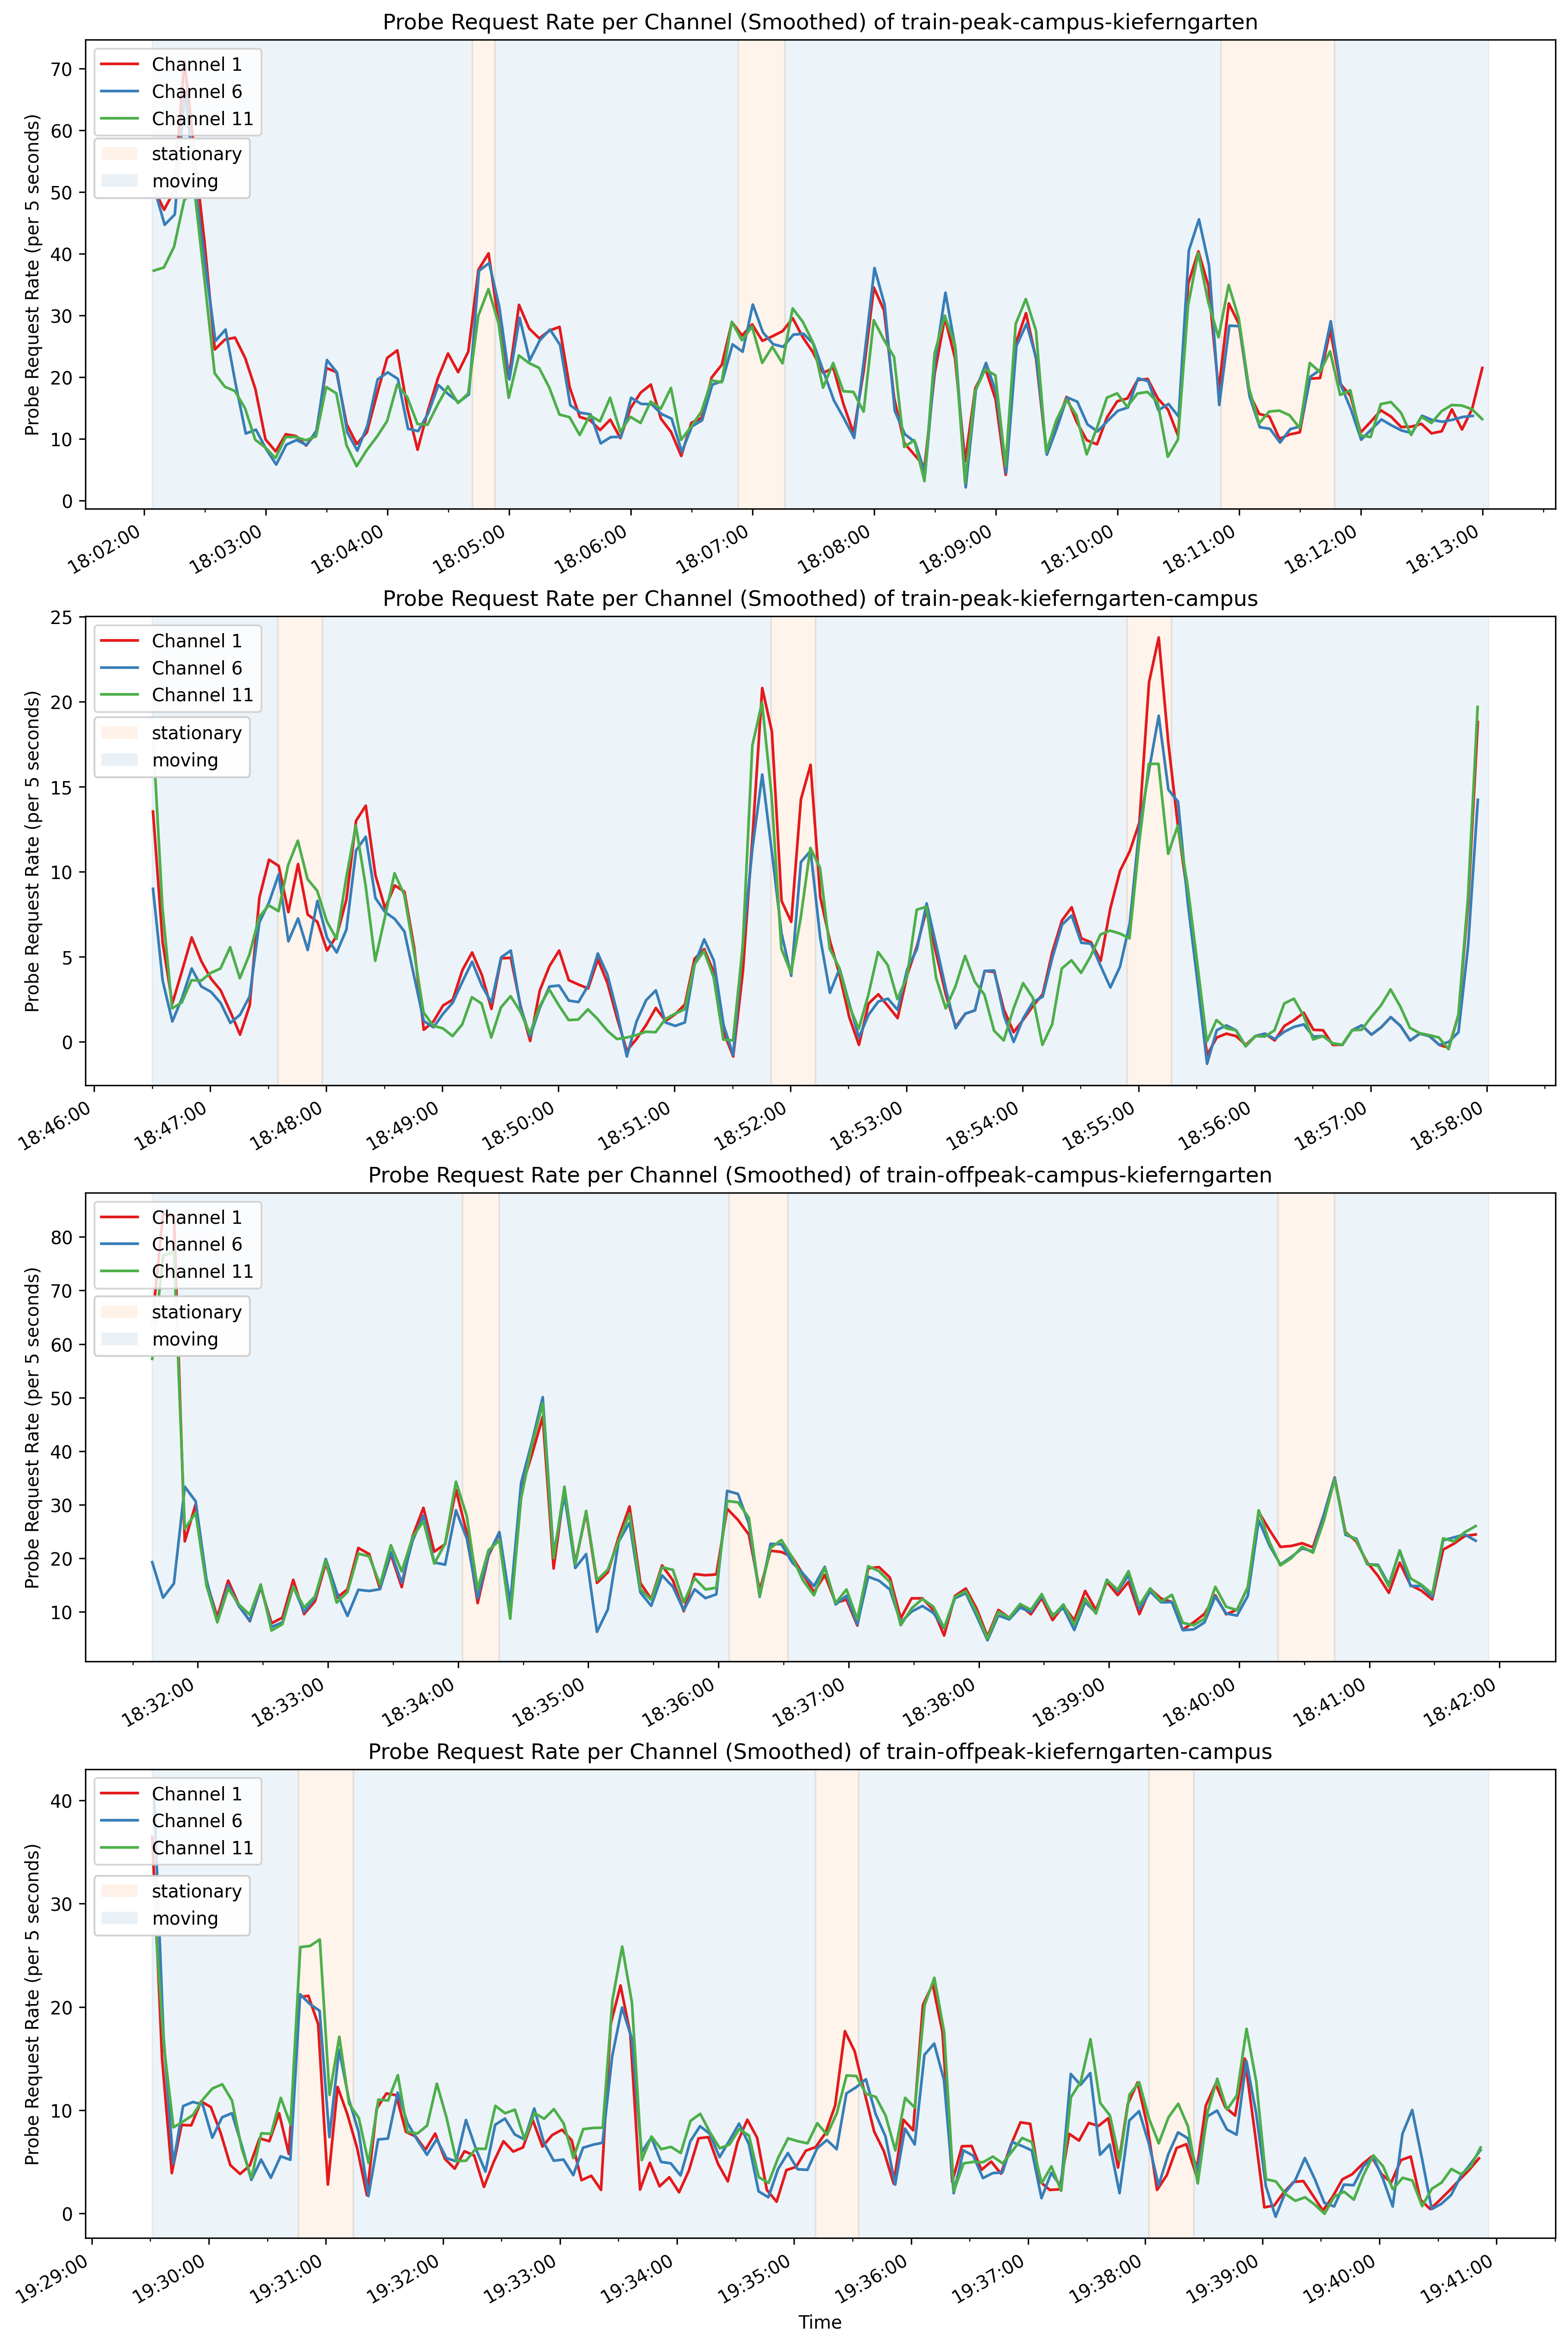
\includegraphics[width=\columnwidth]{images/part1/probe-rate/train-scenarios.png}
    \caption{Packet Arrival Rates for the Train Scenarios}
    \label{fig:train_packet_arrival_rate}
\end{figure}

As can be seen, when a train is at a station, we observe a peak in the probe request rate, which is caused by people waiting for the train to arrive and then entering the train. This is best visible in the peak scenarios, especially in the train-peak-kieferngarten-campus scenario. However, there are other, unexplained peaks in the probe request rate, which can be caused by external factors, such as a passing train, a train passing by an area with a comparable crowd.

Additionally, if everyone at the station were to enter the train, we would expect the probe request rate to remain high after the peak, but it drops off quickly. We theorize that the reason why we see the probe rates drop significantly after the train leaves the station is that there are usually more people waiting for other trains at the stations, not boarding the train where the capturing took place.

Finally, similar to the station scenarios, both in the cumulative packet counts (\cref{fig:train_cumulative_packet_counts}) and the packet arrival rates (\cref{fig:train_packet_arrival_rate}), we can clearly identify the peak and off-peak scenarios, as the peak scenarios display higher packet counts and arrival rates than the off-peak scenarios.

\subsubsection{Packet Counts per MAC Address}
\label{sec:part-1/train/packet-counts-per-mac}
After observing the time series of the packet counts and arrival rates, we now turn our focus to the packet counts per MAC address. The packet counts per top 20 MAC addresses (with respect to the total packet counts) are shown in \cref{fig:train_packet_counts_per_mac}. We also present the number of packets sent by the devices we used in the capture process in \cref{tab:known_devices_train}.

\begin{table}[ht]
    \centering
    \resizebox{\columnwidth}{!}{
    \begin{tabular}{|l|ccc|}
        \hline
        \textbf{Scenario} & \textbf{Controller Laptop} & \textbf{Smartphone} & \textbf{Raspberry Pi} \\
        \hline
        train-peak-campus-kieferngarten & 1 & 0 & 0 \\
        \hline
        train-peak-kieferngarten-campus & 3 & 0 & 0 \\
        \hline
        train-offpeak-campus-kieferngarten & 3 & 0 & 0 \\
        \hline
        train-offpeak-kieferngarten-campus & 2 & 0 & 0 \\
        \hline
    \end{tabular}
    }
    \caption{Packet counts of known devices in train scenarios.}
    \label{tab:known_devices_train}
\end{table}

\begin{figure}
    \centering
    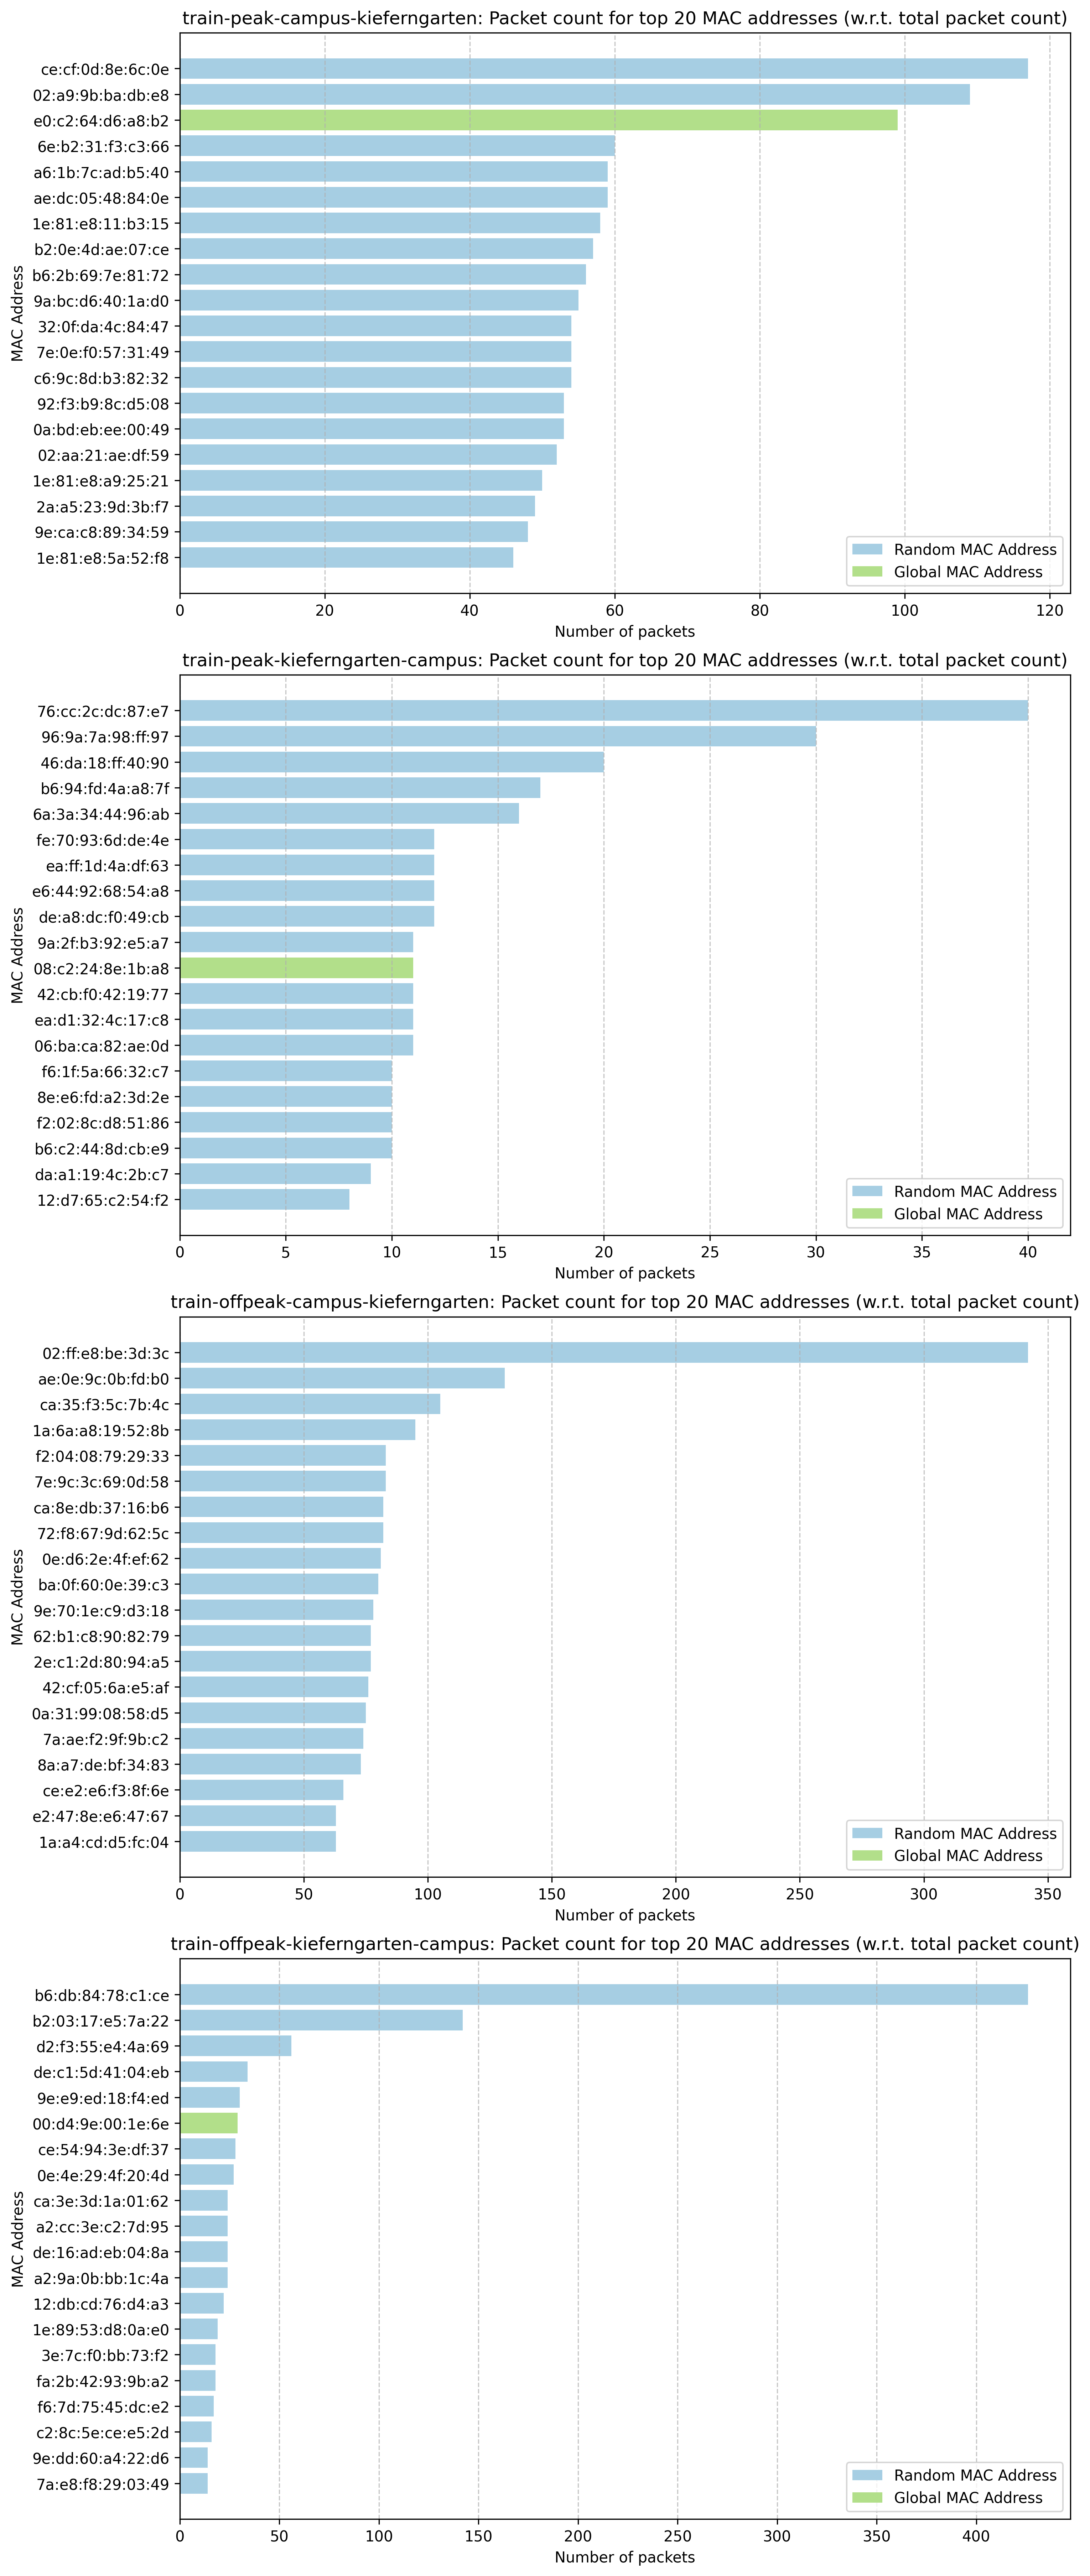
\includegraphics[width=\columnwidth]{images/part1/packet-counts/top-macs-train-scenarios.png}
    \caption{Packet Counts per MAC Address for the Train Scenarios}
    \label{fig:train_packet_counts_per_mac}
\end{figure}

Unlike the station scenarios, we see that the top MAC addresses in the off-peak scenarios have significantly higher packet counts than the peak scenarios. This is precisely what we hypothesized as possible in \cref{sec:part-1/station/packet-counts-per-mac}. We explained that the apparent difference between the peak and off-peak scenarios in the station scenarios is coincidental, as the number of probe requests a device sends is not directly correlated with the number of people present at the station. In this case, it happened to be that there were some devices present in the off-peak scenario that were sending probe requests more frequently than ones present in the peak scenarios.

\subsubsection{RSSI Distribution}
\label{sec:part-1/train/rssi-distribution}

The RSSI distribution for the train scenarios is shown in \cref{fig:train_rssi_distribution}.
\begin{figure}
    \centering
    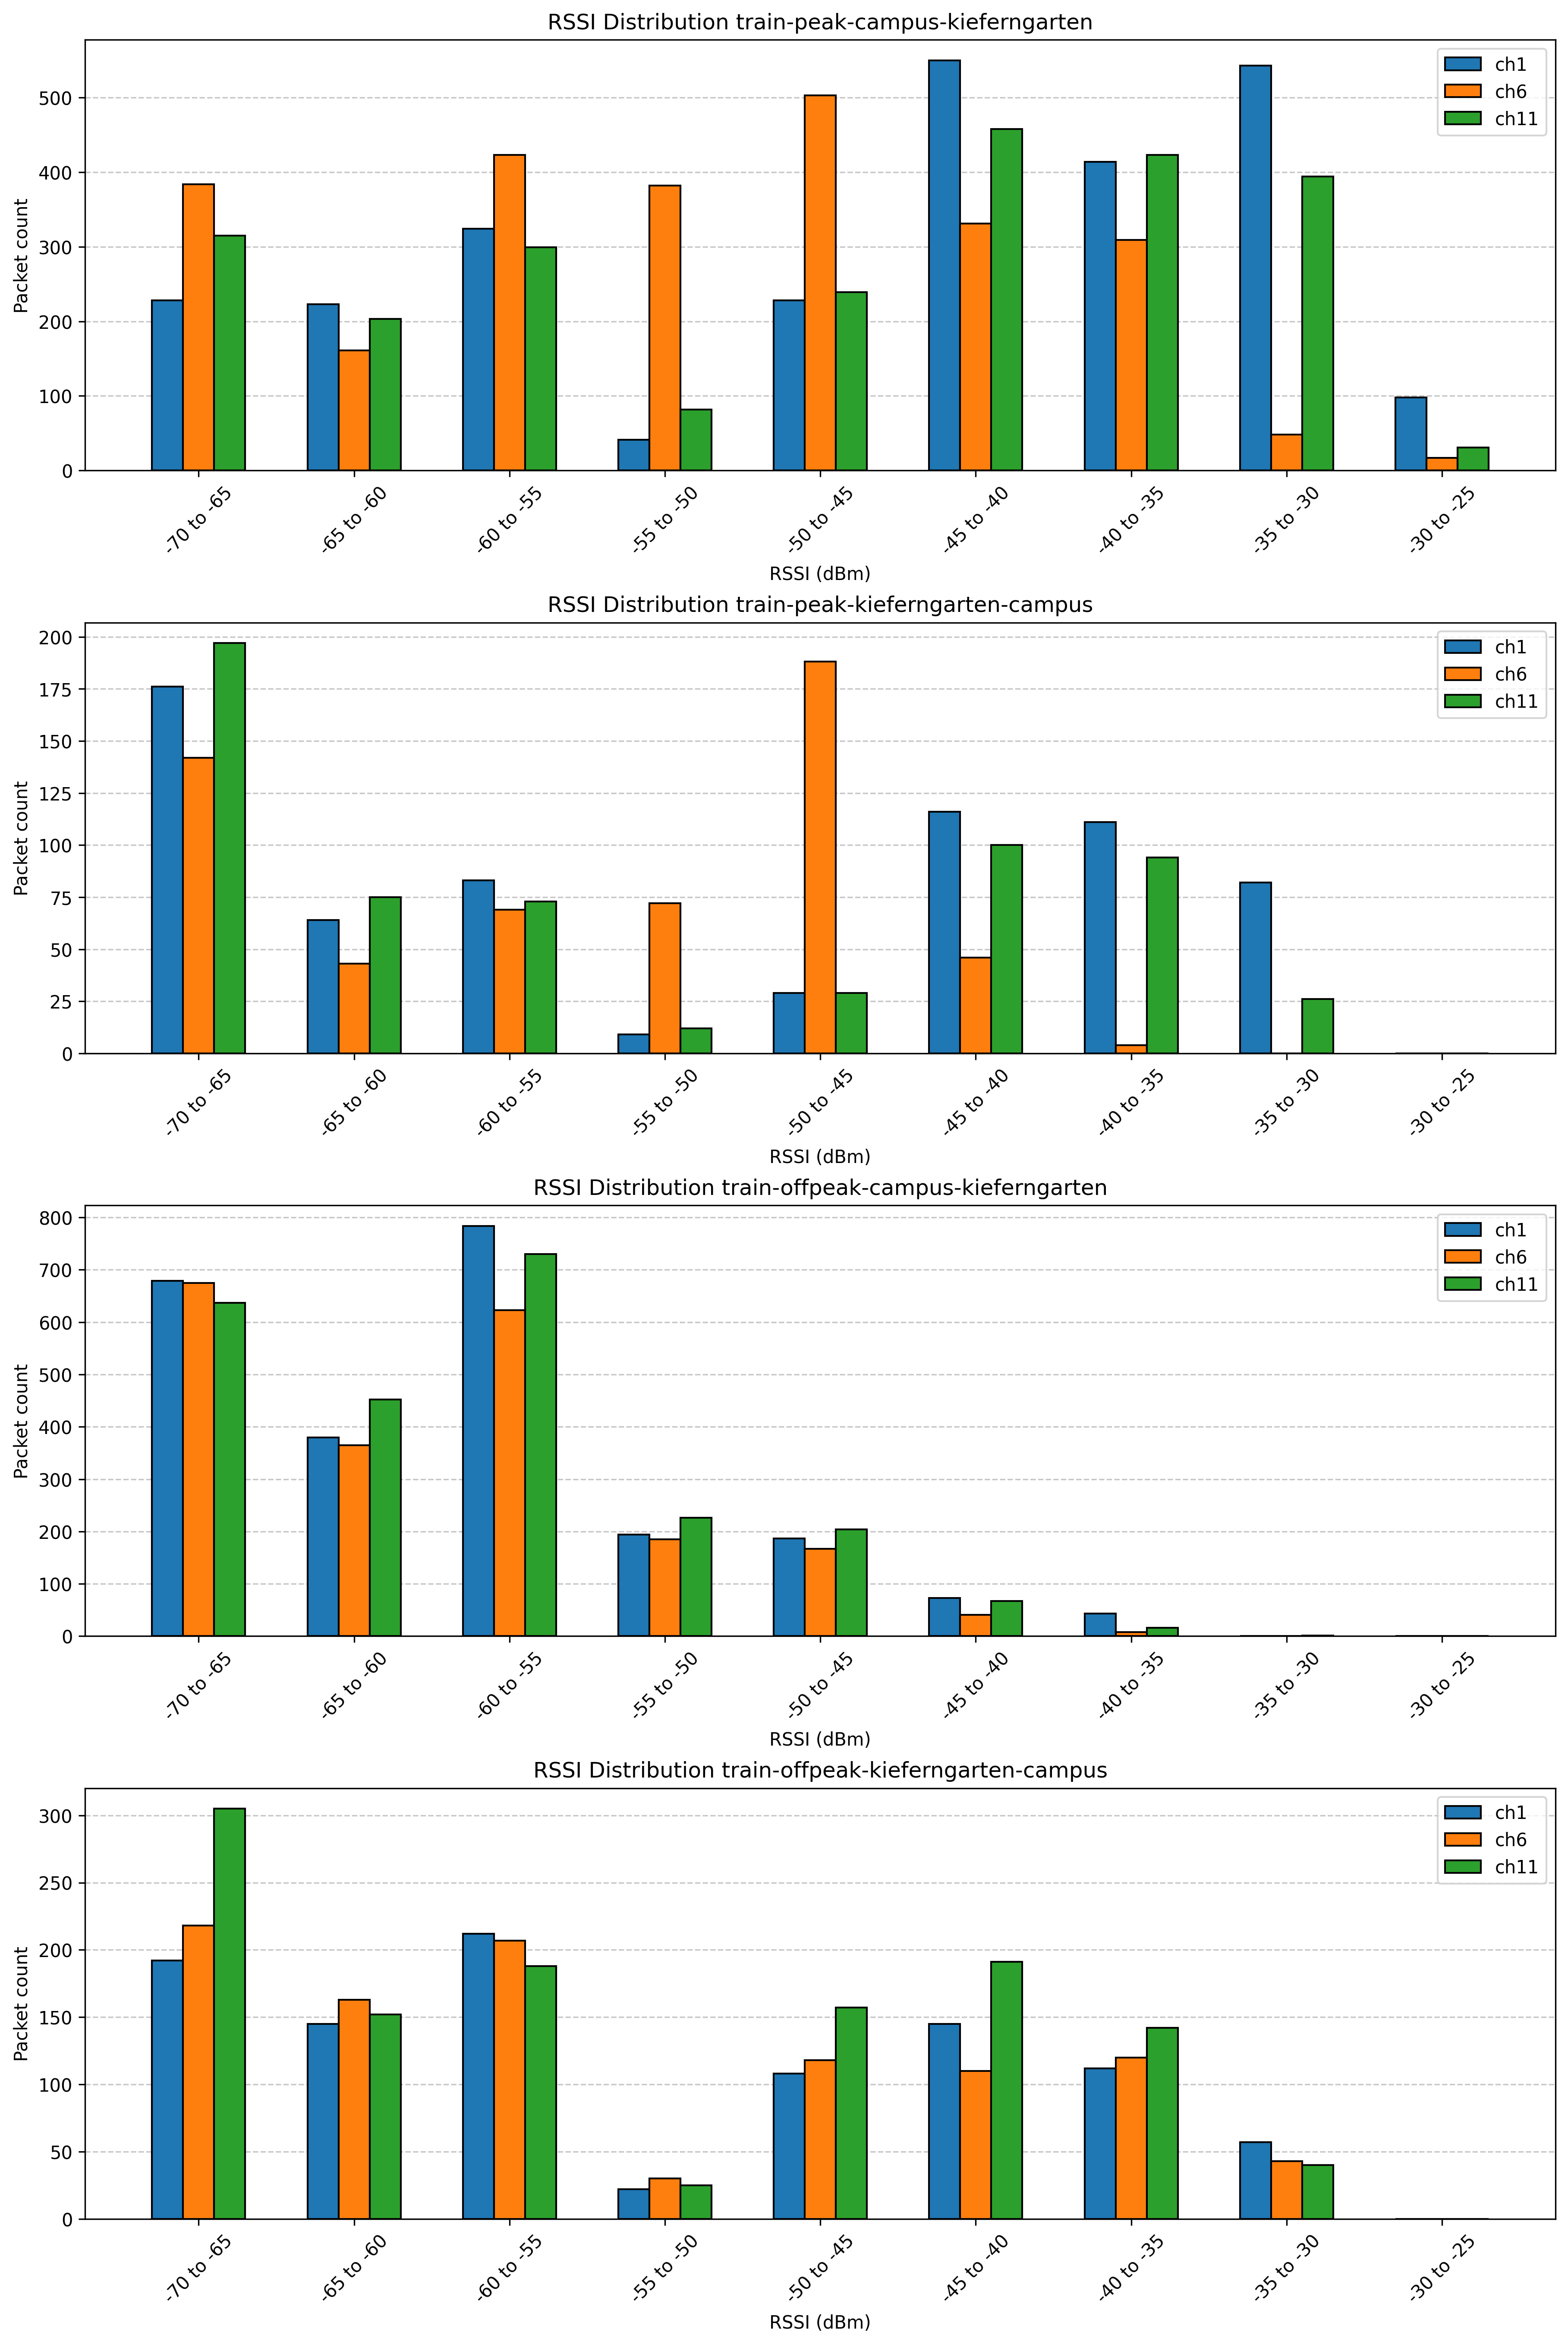
\includegraphics[width=\columnwidth]{images/part1/rssi/train-scenarios.png}
    \caption{RSSI Distribution for the Train Scenarios}
    \label{fig:train_rssi_distribution}
\end{figure}

Similar to the station scenarios, we observe a dip in the RSSI distribution around -50 to -55 dBm. However, this time, our hypothesis that the dip is caused by people gathering around benches is not valid, as there are no benches in the train, and people are usually more evenly distributed in the train. This leads us to believe that our initial hypothesis was wrong. However, we could not come up with a better explanation that would explain this dip that we see in all of the scenarios.

The only other noteworthy observation here is that in the train-offpeak-campus-kieferngarten scenario, we don't see as many packets with an RSSI value of -35 to -25 dBm, which is caused by the exceptionally low number of people in the specific car where the capture was done. During the capture, only 3 people were in the car, which is why we see so few packets with such high RSSI values.

\subsubsection{RSSI Distribution per MAC Address}
\label{sec:part-1/train/rssi-distribution-per-mac}
Similar to the station scenarios, we now turn our attention to the RSSI distribution per MAC address with the same goal in mind.
However, this time, we do not see any of the devices we used to control the capture process in the top 20 MAC addresses, as only the controller laptop was sending probe requests, and it sent less than 5 packets in all of the train scenarios. Among the remaining MAC addresses, we did not observe any significant patterns; thus, we omit the corresponding figure for the sake of briefness.

\subsubsection{MAC Address Randomization}
\label{sec:part-1/train/mac-randomization}
Similar to the station scenarios, we now present the results of the MAC address randomization analysis based on unique MAC addresses. The results are shown in \cref{tab:mac_randomization_station} and \cref{fig:train_mac_randomization}.

\begin{table}[ht]
    \centering
    \caption{MAC Address Randomization Ratios in Train Scenarios}
    \label{tab:mac_randomization_train}
    \resizebox{\columnwidth}{!}{
    \begin{tabular}{|l|r|r|r|r|}
        \hline
        \textbf{Scenario} & \textbf{Random} & \textbf{Global} & \textbf{Total} & \textbf{Random Ratio (\%)} \\
        \hline
        train-peak-campus-kieferngarten & 1976 & 11 & 1987 & 99.45\% \\
        train-peak-kieferngarten-campus & 673 & 5 & 678 & 99.26\% \\
        train-offpeak-campus-kieferngarten & 723 & 3 & 726 & 99.59\% \\
        train-offpeak-kieferngarten-campus & 1189 & 5 & 1194 & 99.58\% \\
        \hline
    \end{tabular}
    }
\end{table}

\begin{figure}
    \centering
    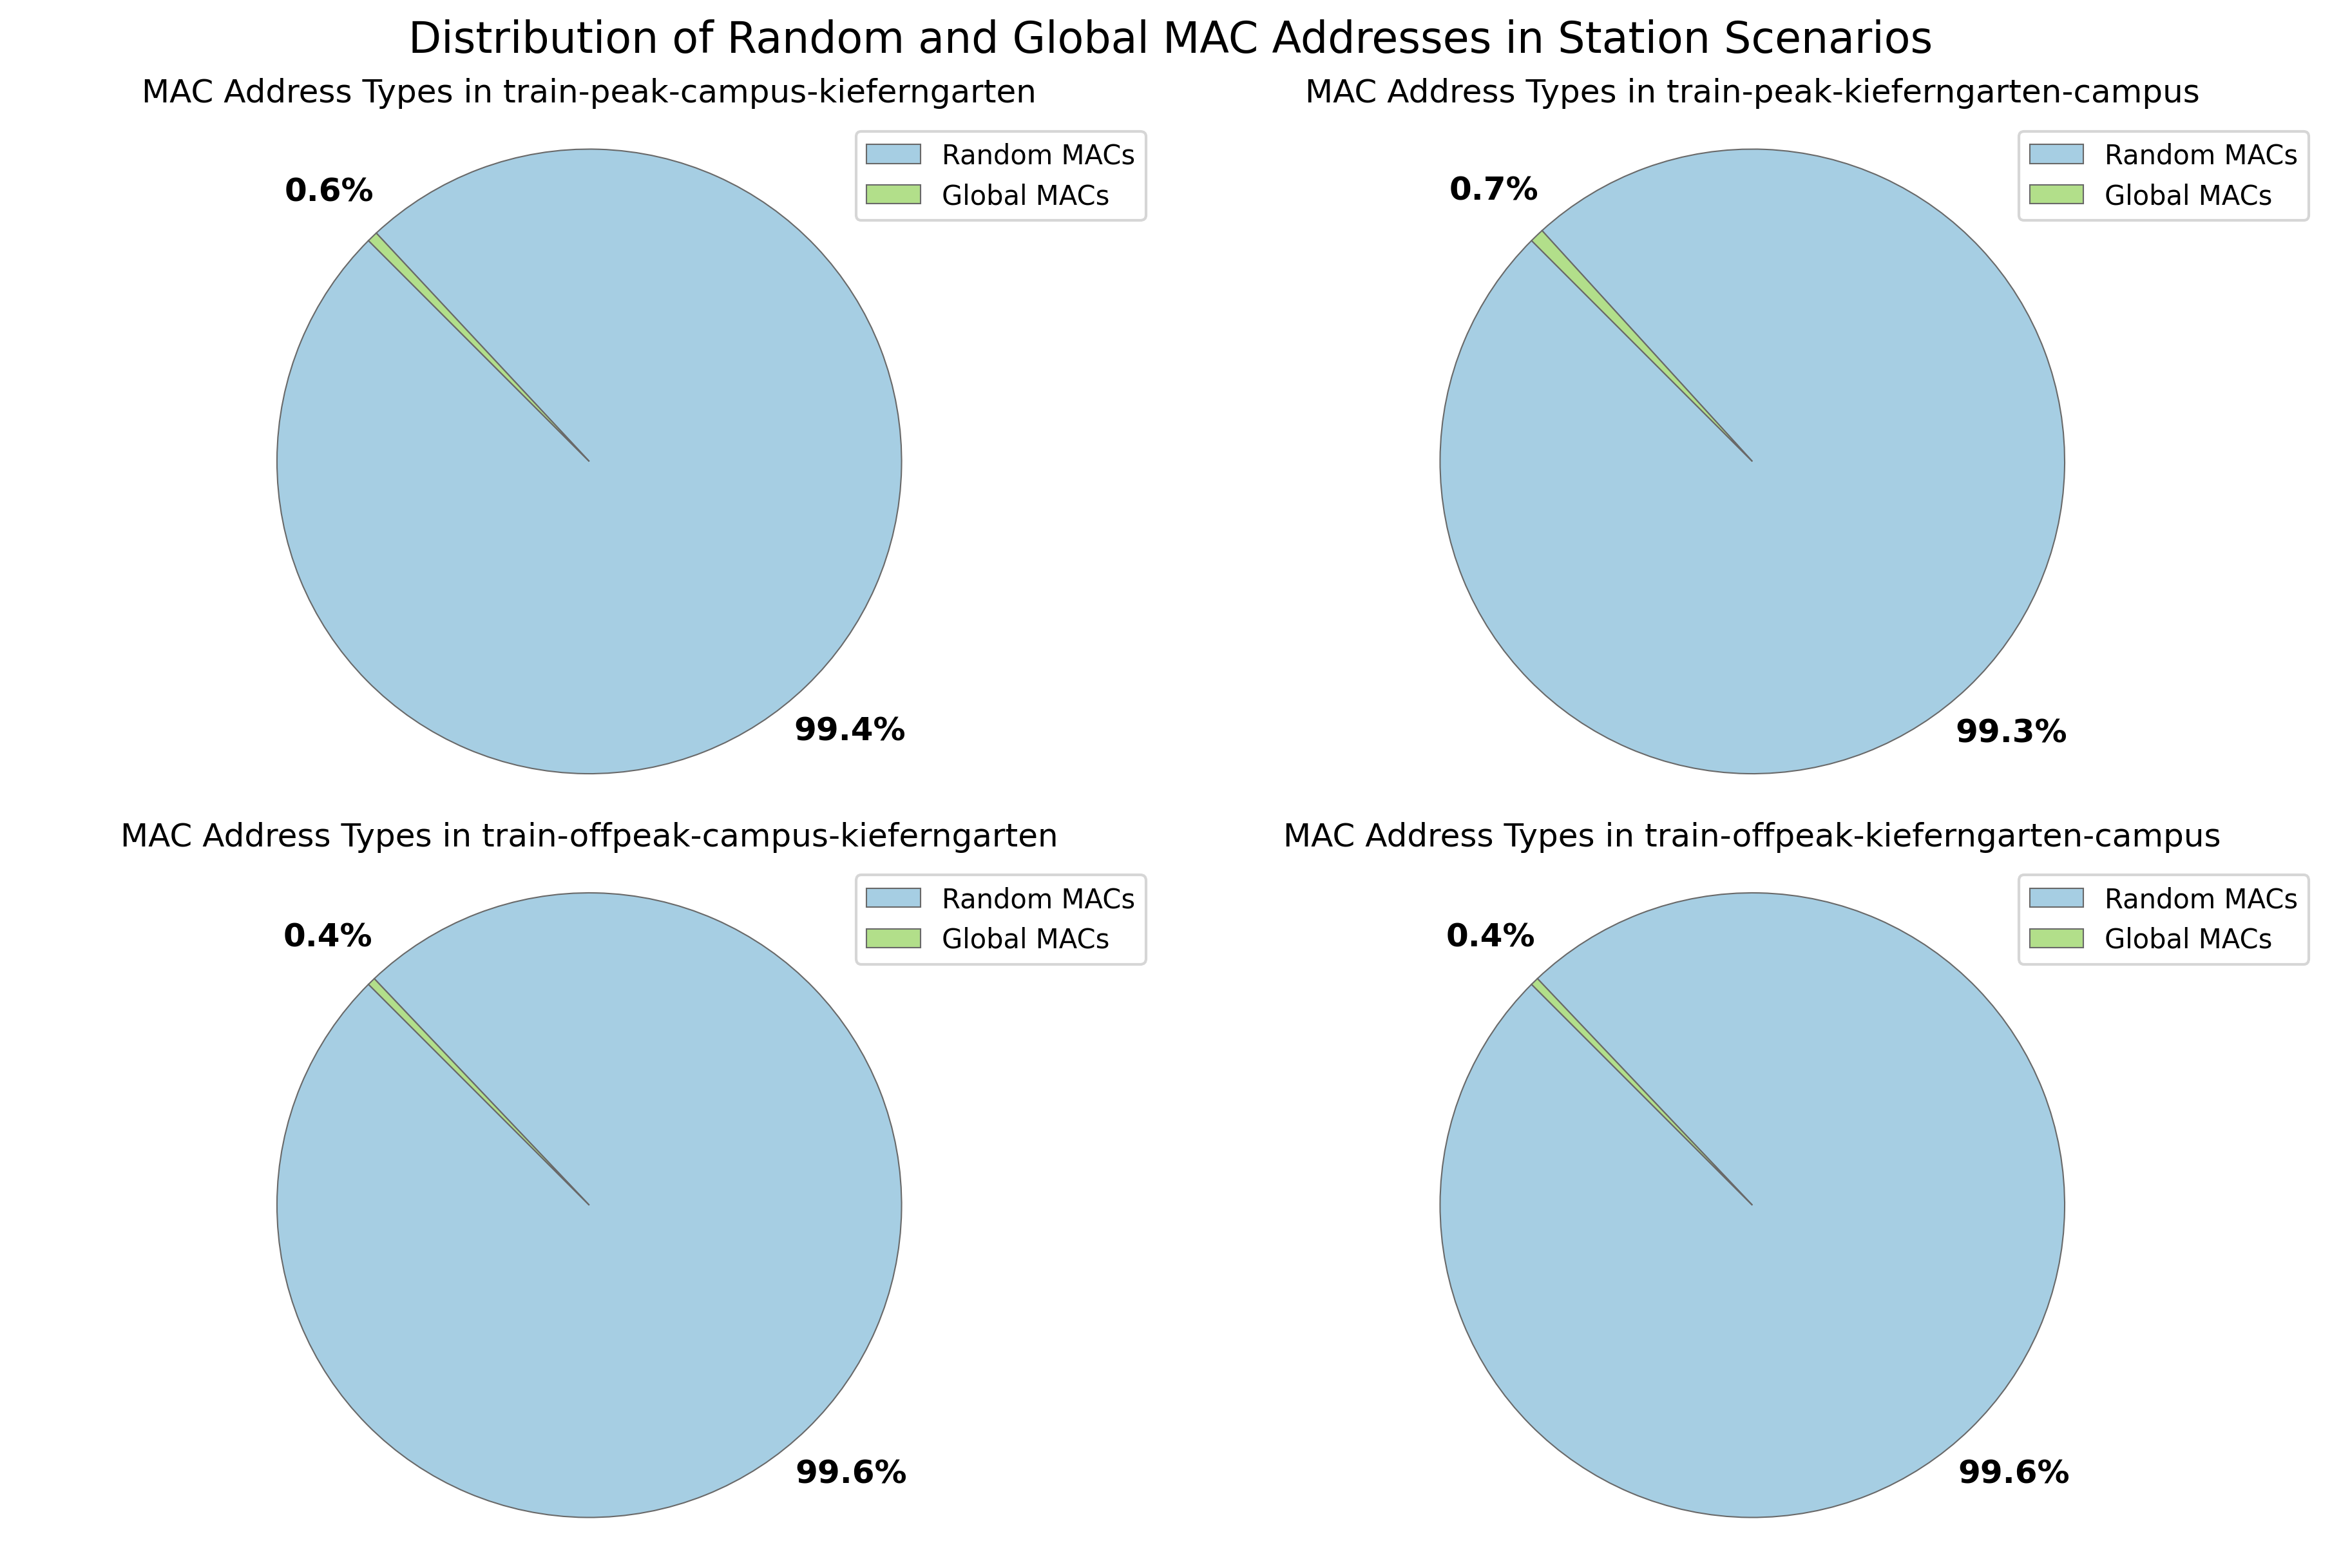
\includegraphics[width=\columnwidth]{images/part1/mac-address-types/train-scenarios.png}
    \caption{MAC Address Randomization for the Train Scenarios}
    \label{fig:train_mac_randomization}
\end{figure}

Similarly, we did not find any correlation between the population and the randomized MAC address ratios in the train scenarios either.

\subsubsection{MAC Address Randomization by Packet Count}
\label{sec:part-1/train/mac-randomization-packet-count}
As in the station scenarios, we present the results of the MAC address randomization analysis based on total packet counts. The results are shown in \cref{tab:mac_randomization_train_packets} and \cref{fig:train_mac_randomization_packet_count}.

\begin{table}[ht]
    \centering
    \caption{Packet-based MAC Address Randomization Ratios in Train Scenarios}
    \label{tab:mac_randomization_train_packets}
    \resizebox{\columnwidth}{!}{
    \begin{tabular}{|l|r|r|r|r|}
        \hline
        \textbf{Scenario} & \textbf{Random MAC Pkts} & \textbf{Global MAC Pkts} & \textbf{Total Pkts} & \textbf{Random Pkts Ratio (\%)} \\
        \hline
        train-peak-campus-kieferngarten & 7477 & 177 & 7654 & 97.69\% \\
        train-peak-kieferngarten-campus & 1816 & 24 & 1840 & 98.70\% \\
        train-offpeak-campus-kieferngarten & 6696 & 41 & 6737 & 99.39\% \\
        train-offpeak-kieferngarten-campus & 3155 & 47 & 3202 & 98.53\% \\
        \hline
    \end{tabular}
    }
\end{table}

\begin{figure}
    \centering
    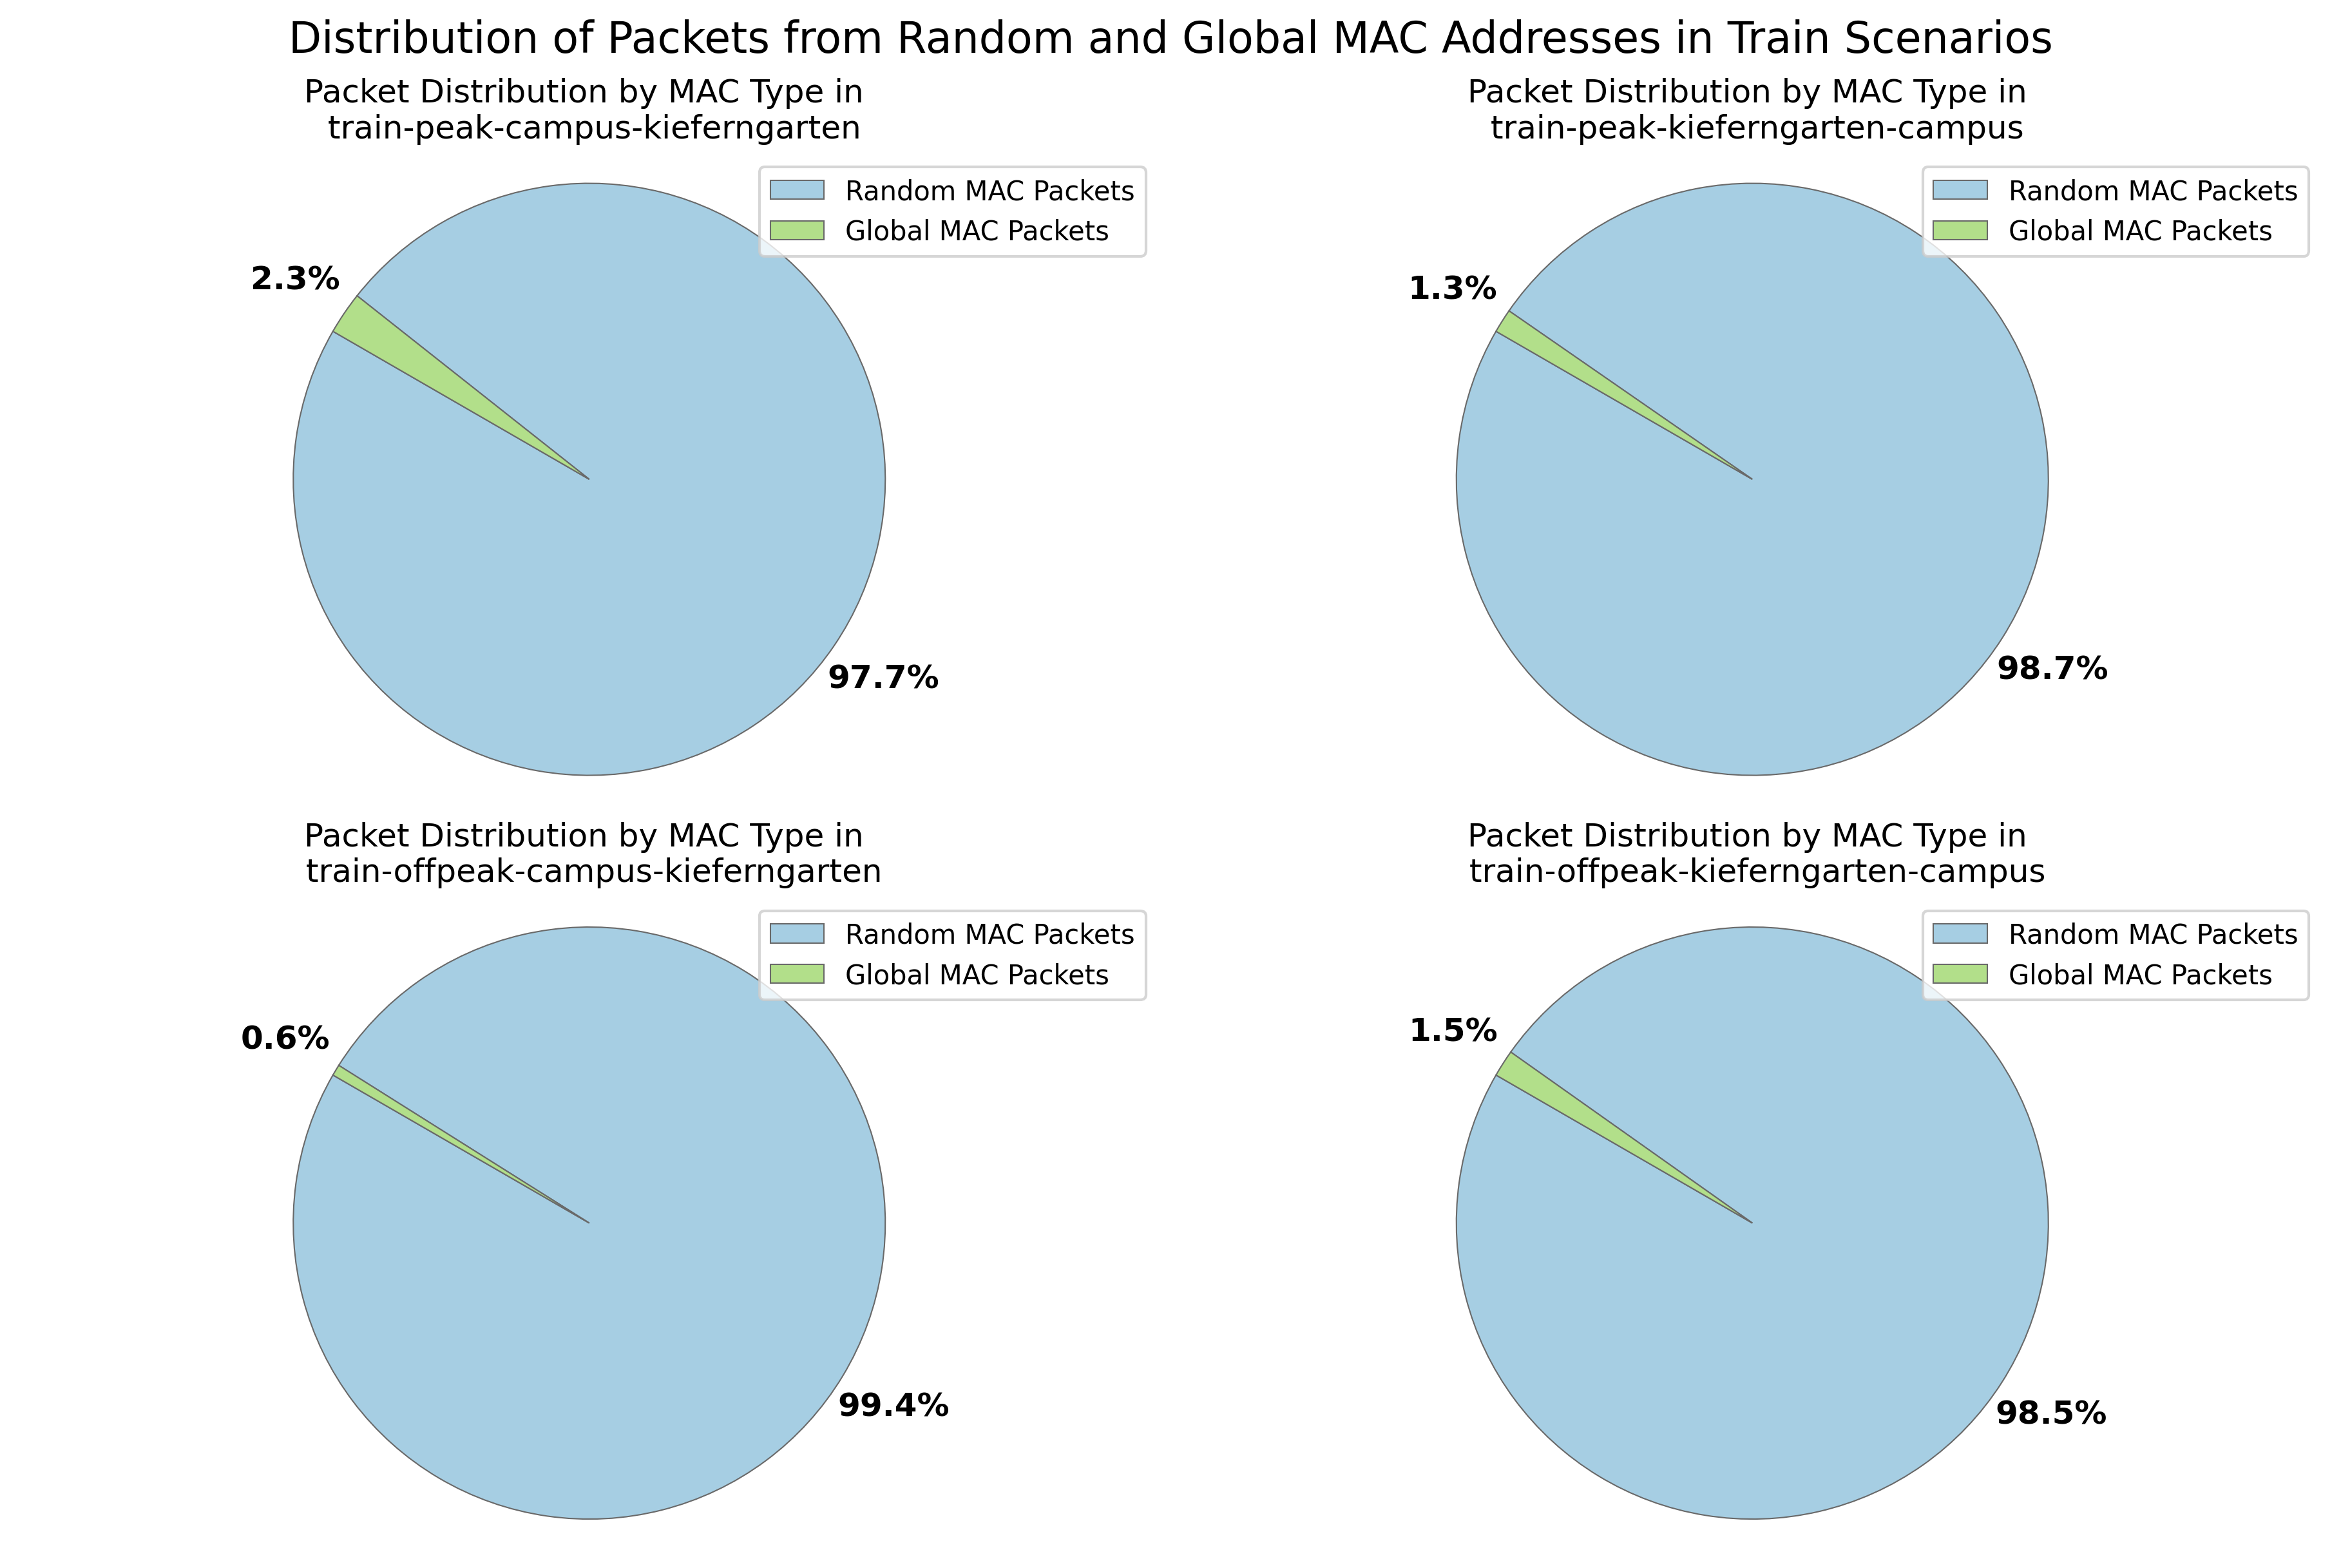
\includegraphics[width=\columnwidth]{images/part1/mac-address-types/train-scenarios-packet-based.png}
    \caption{MAC Address Randomization by Packet Count for the Train Scenarios}
    \label{fig:train_mac_randomization_packet_count}
\end{figure}

\subsubsection{Vendor OUIs}
\label{sec:part-1/train/oui}
We present the top 10 most common vendor OUIs in the train scenarios by unique MAC address count. The results are shown in \cref{tab:train_oui}. Just like in the MAC randomization analysis, we only take into account unique MAC addresses, i.e., the same OUI is counted only once, regardless of how many packets it sends.

\subsubsection{Vendor OUIs by Packet Count}
\label{sec:part-1/train/oui-packet-count}
We now turn our attention to the vendor OUIs by packet count. The results are shown in \cref{tab:train_oui_packet_count}. The results are based on total packet counts, i.e., the same OUI is counted as many times as it sends packets.
\begin{figure}
    \centering
    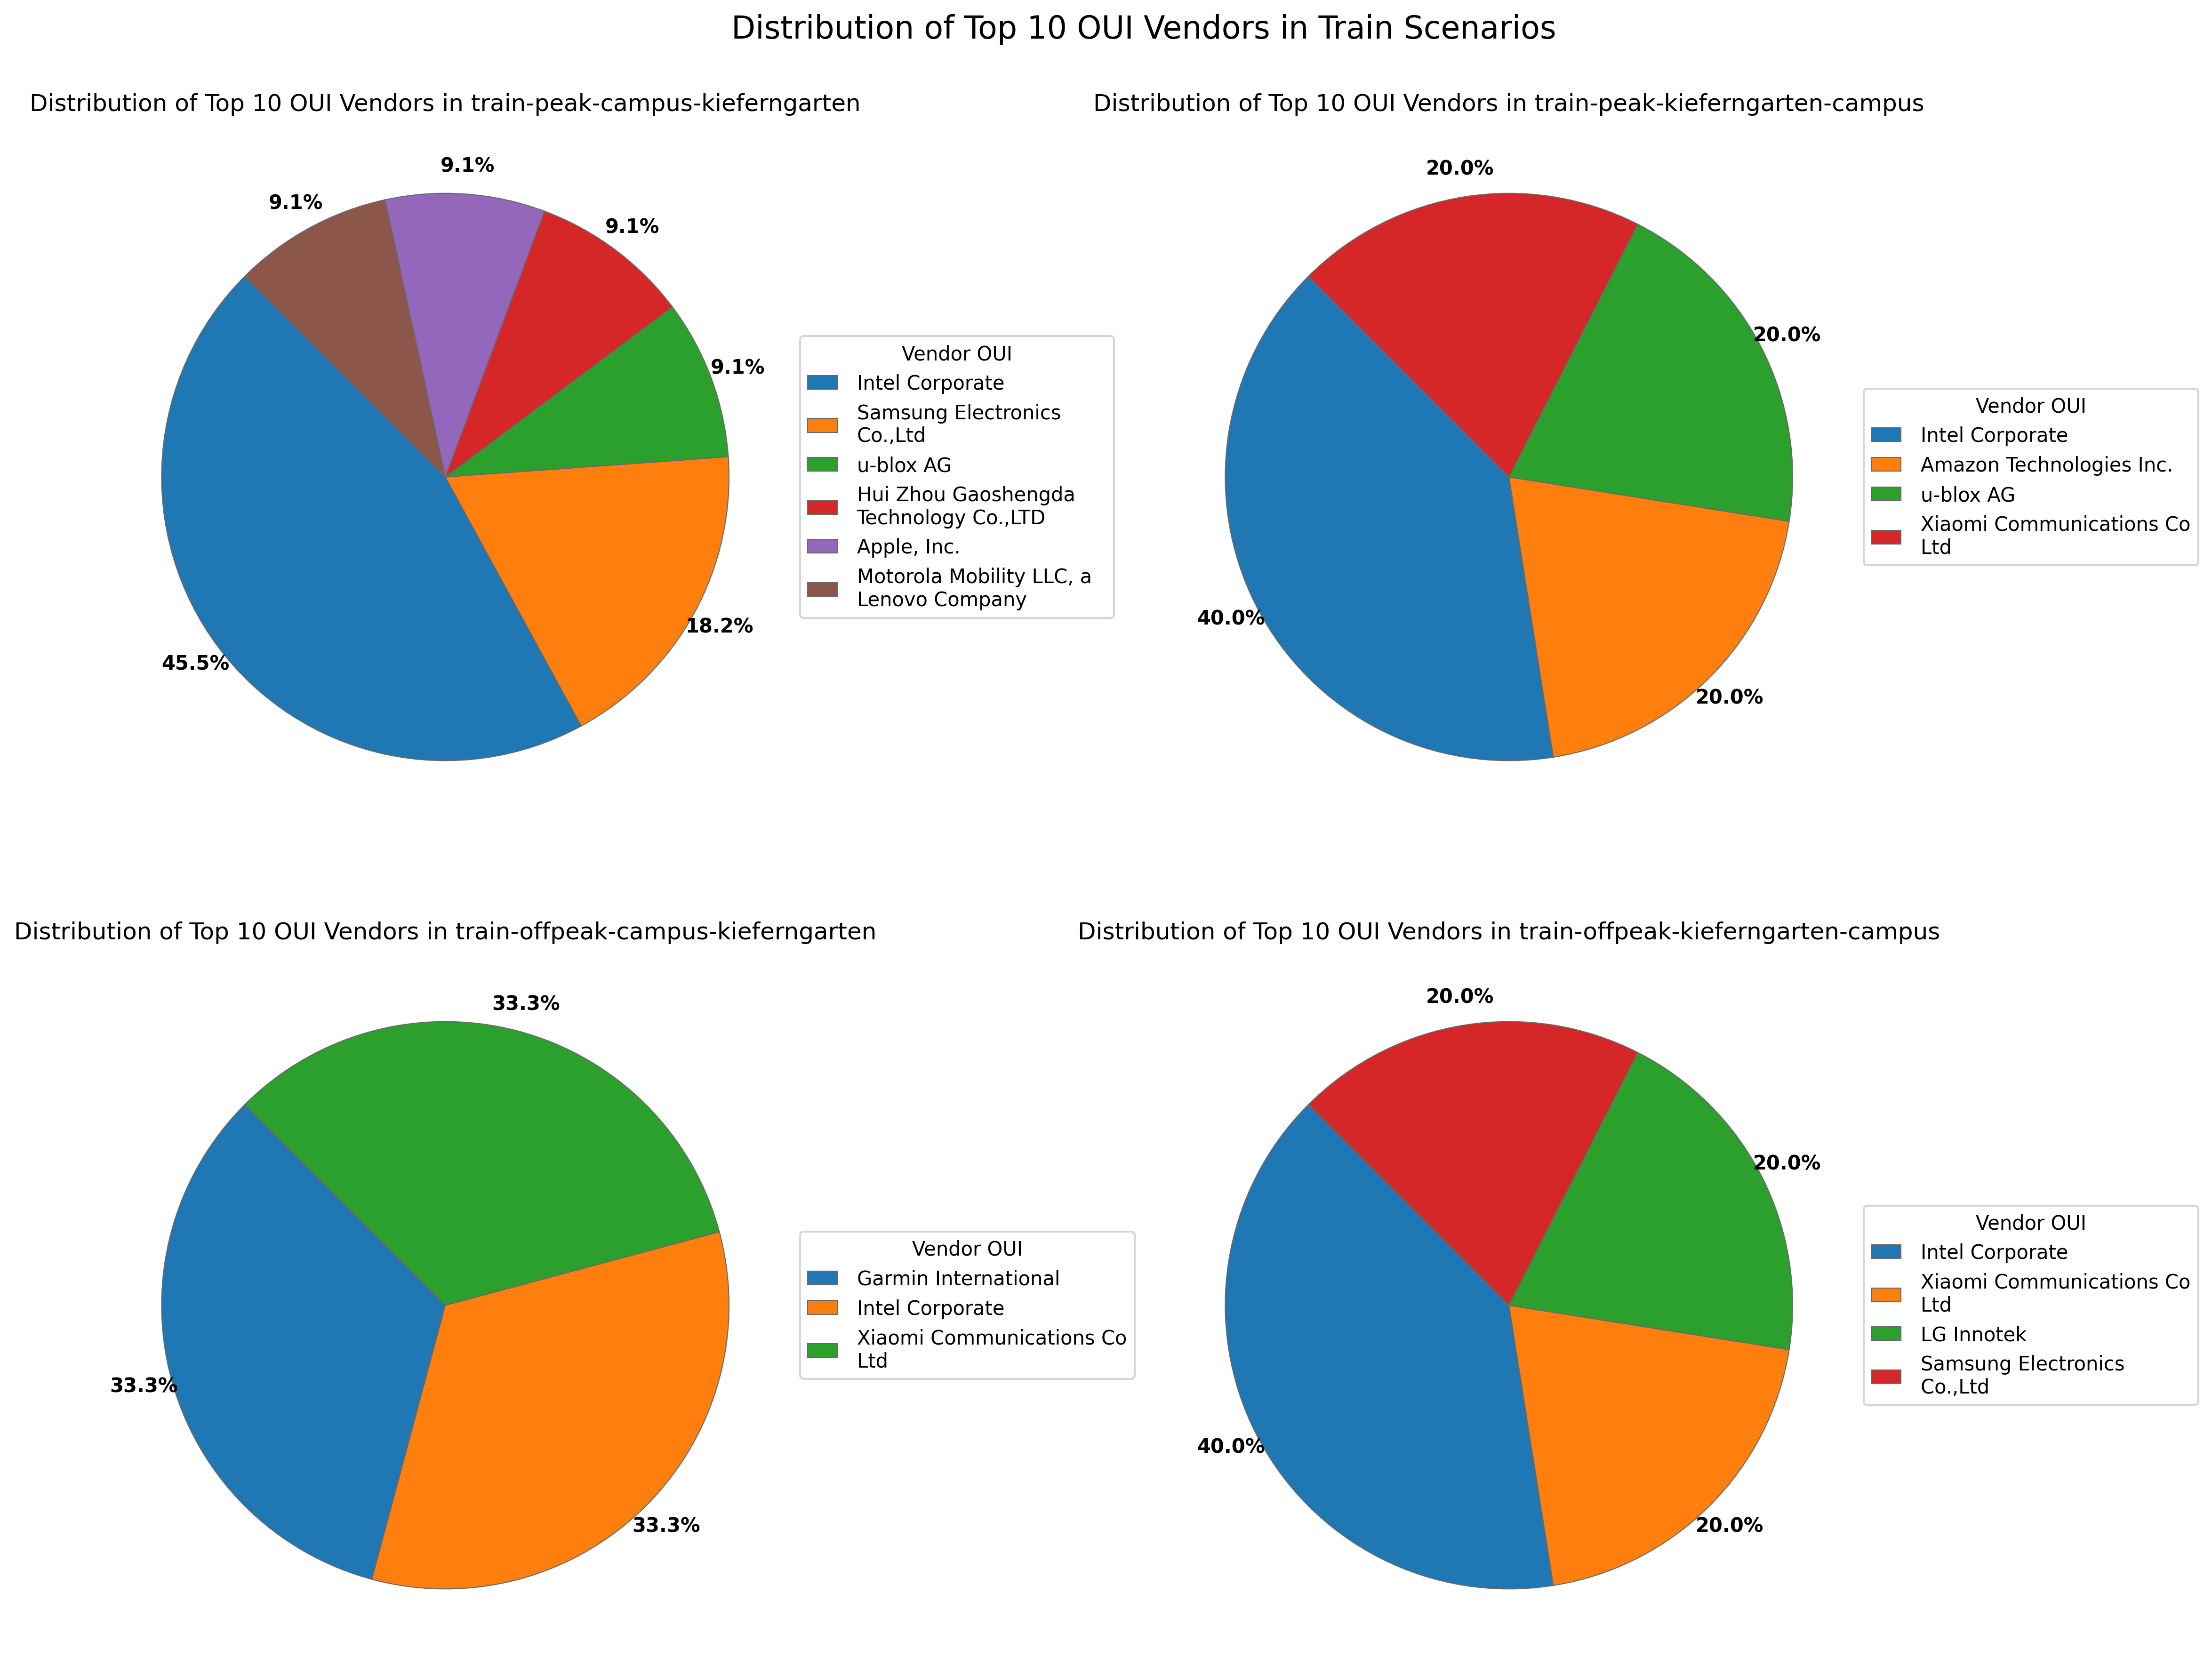
\includegraphics[width=\columnwidth]{images/part1/oui-vendors/train-scenarios.png}
    \caption{Top 10 Vendor OUIs in the Train Scenarios}
    \label{tab:train_oui}
\end{figure}

\begin{figure}
    \centering
    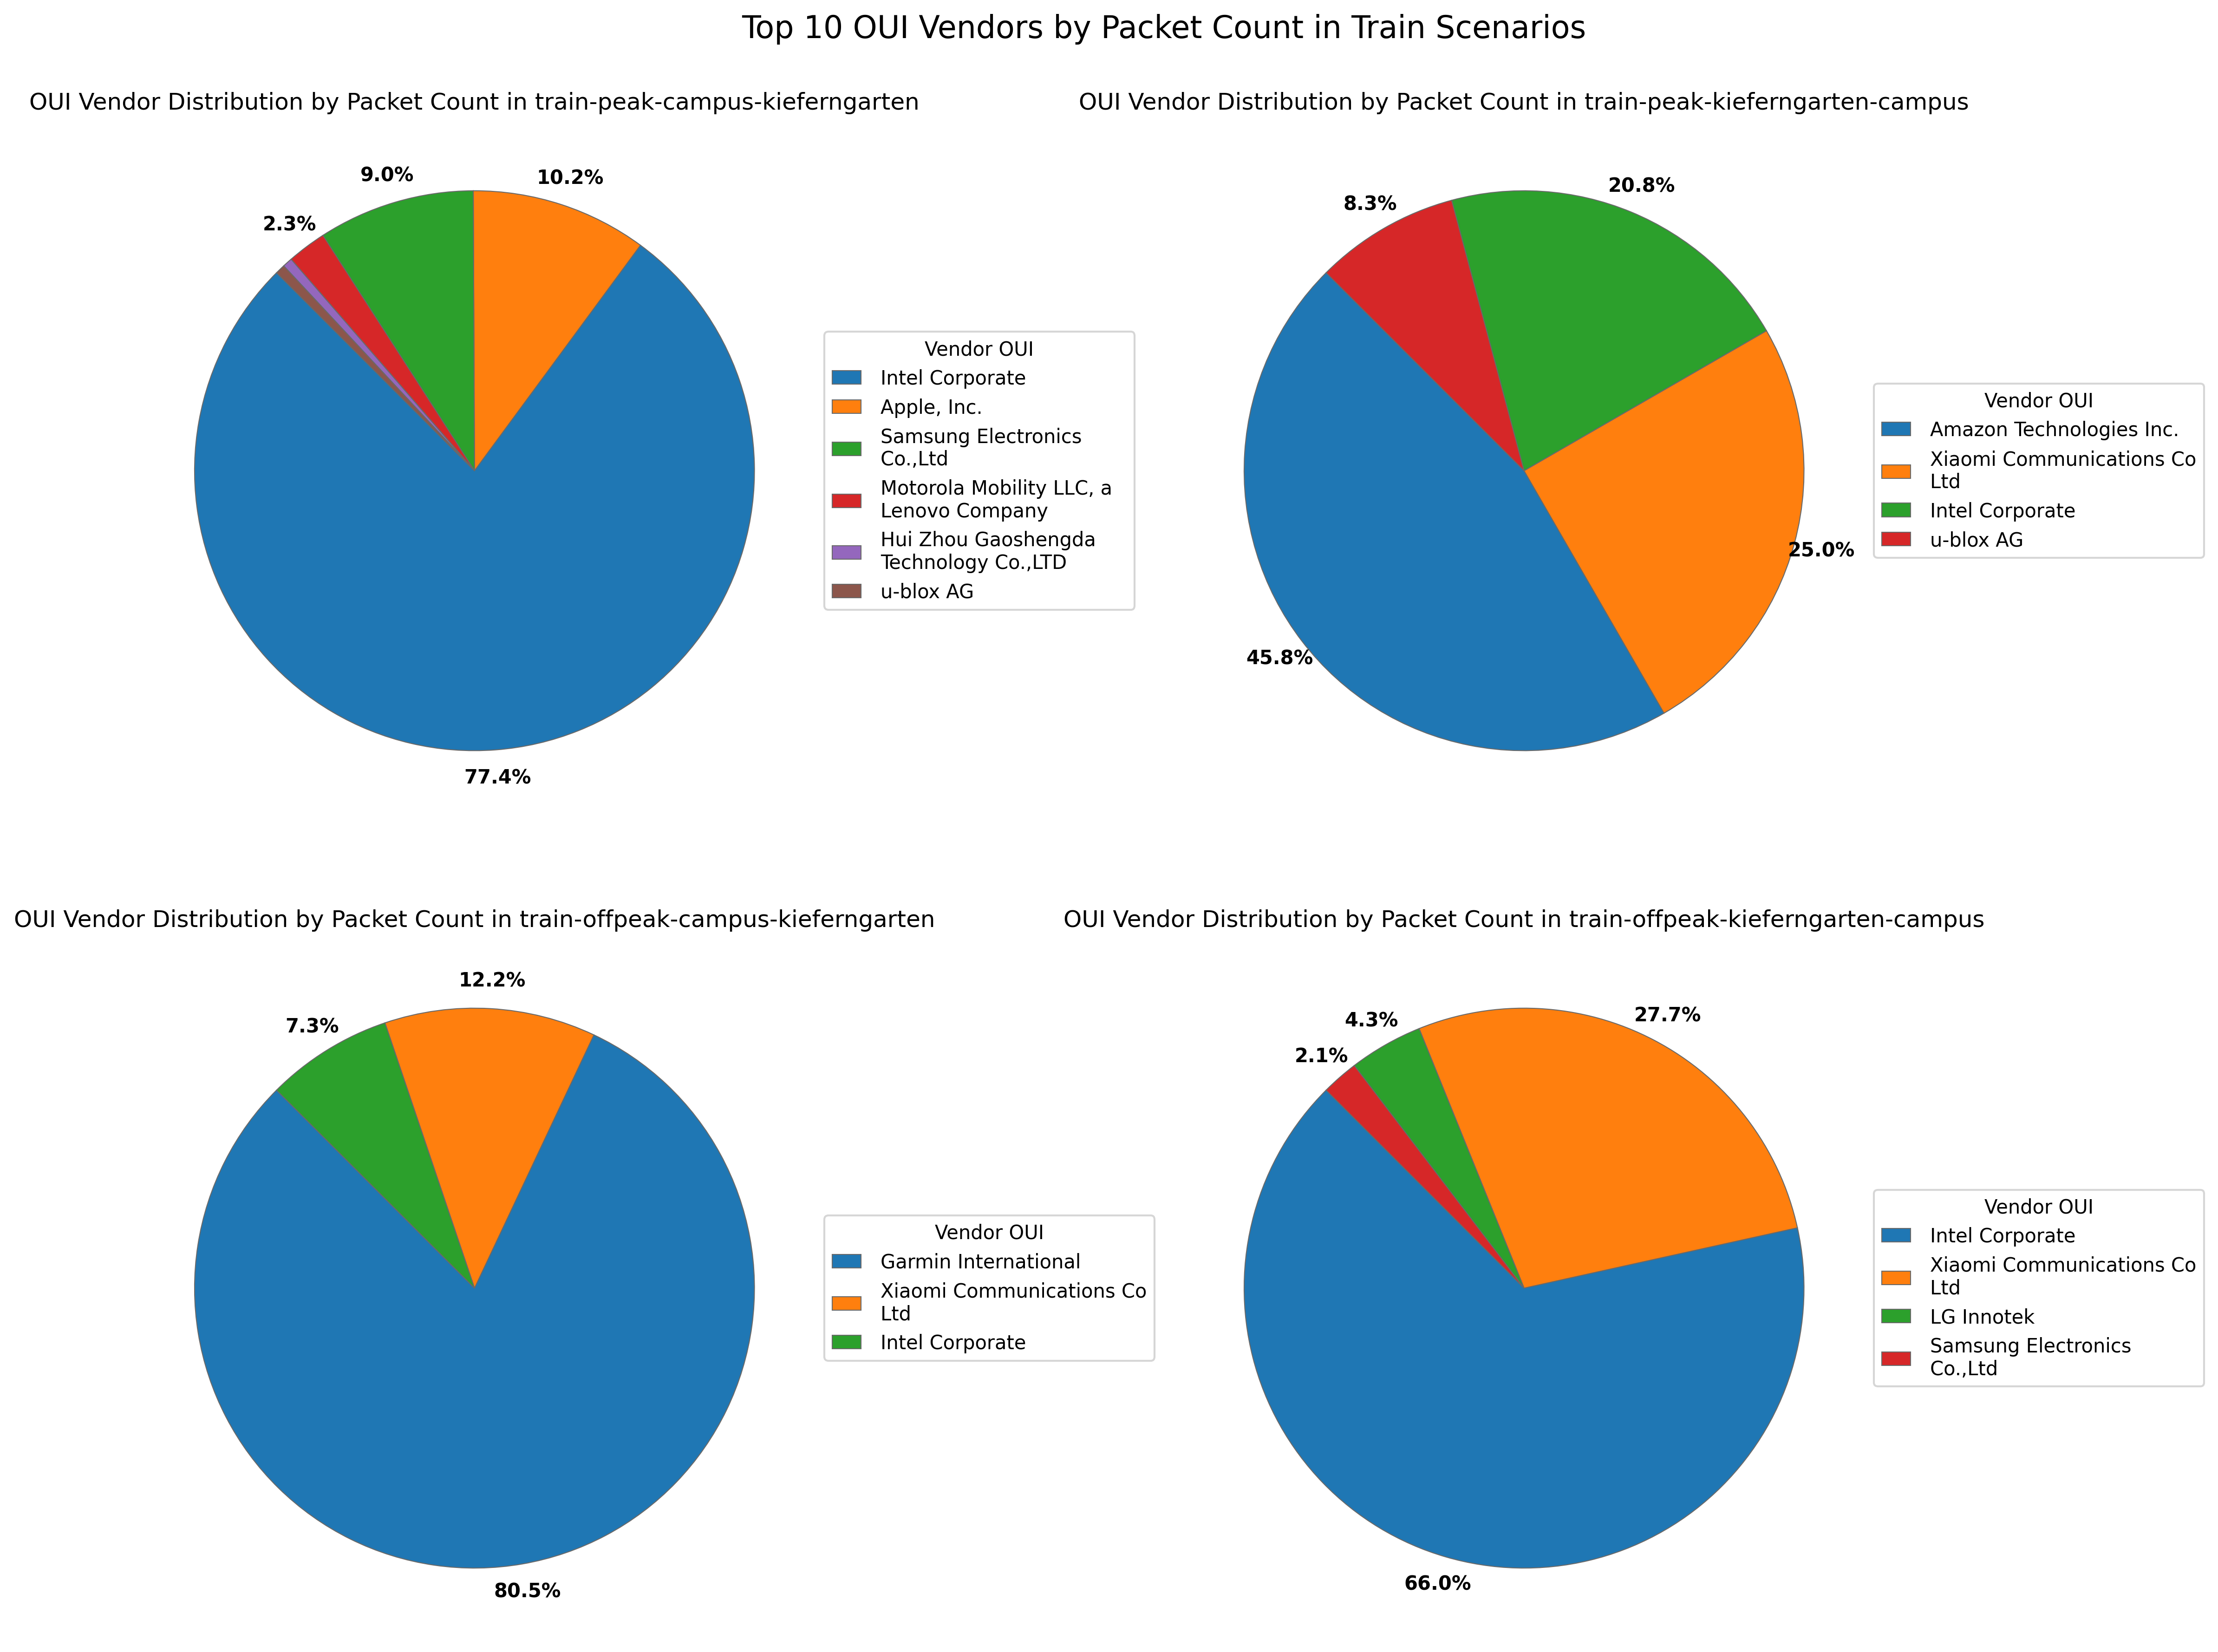
\includegraphics[width=\columnwidth]{images/part1/oui-vendors/train-scenarios-packet-count.png}
    \caption{Top 10 Vendor OUIs by Packet Count in the Train Scenarios}
    \label{tab:train_oui_packet_count}
\end{figure}

The analysis we did in the corresponding section in the station results may not apply here, because in the train scenarios, the devices may leave the environment along with their owners, which may lead to a different probe request share. We assumed this is not the case in the station scenarios, as people usually wait until the train arrives; therefore, they don't leave the environment until the train leaves.

\subsubsection{SSIDs}
\label{sec:part-1/train/ssids}

Again, just like in the station scenario results, we present the SSID distribution of the probe requests captured in the train scenarios. We present the number of SSID set vs SSID not set packets and their ratios in the train scenarios in \cref{tab:ssid_presence_train} and \cref{fig:ssid_presence_train} respectively. We then finalize our analysis of the train scenarios with the top 10 most common SSIDs in the train scenarios in \cref{fig:train_ssids}.

\begin{table}[ht]
    \centering
    \caption{Packet Distribution by SSID Presence in Train Scenarios}
    \label{tab:ssid_presence_train}
    \resizebox{\columnwidth}{!}{
    \begin{tabular}{|l|r|r|r|r|}
        \hline
        \textbf{Scenario} & \textbf{SSID Set} & \textbf{SSID Not Set} & \textbf{Total Packets} & \textbf{SSID Set Ratio (\%)} \\
        \hline
        train-peak-campus-kieferngarten & 2387 & 5267 & 7654 & 31.19\% \\
        train-peak-kieferngarten-campus & 306 & 1534 & 1840 & 16.63\% \\
        train-offpeak-campus-kieferngarten & 2704 & 4033 & 6737 & 40.14\% \\
        train-offpeak-kieferngarten-campus & 665 & 2537 & 3202 & 20.77\% \\
        \hline
    \end{tabular}
    }
\end{table}

\begin{figure}
    \centering
    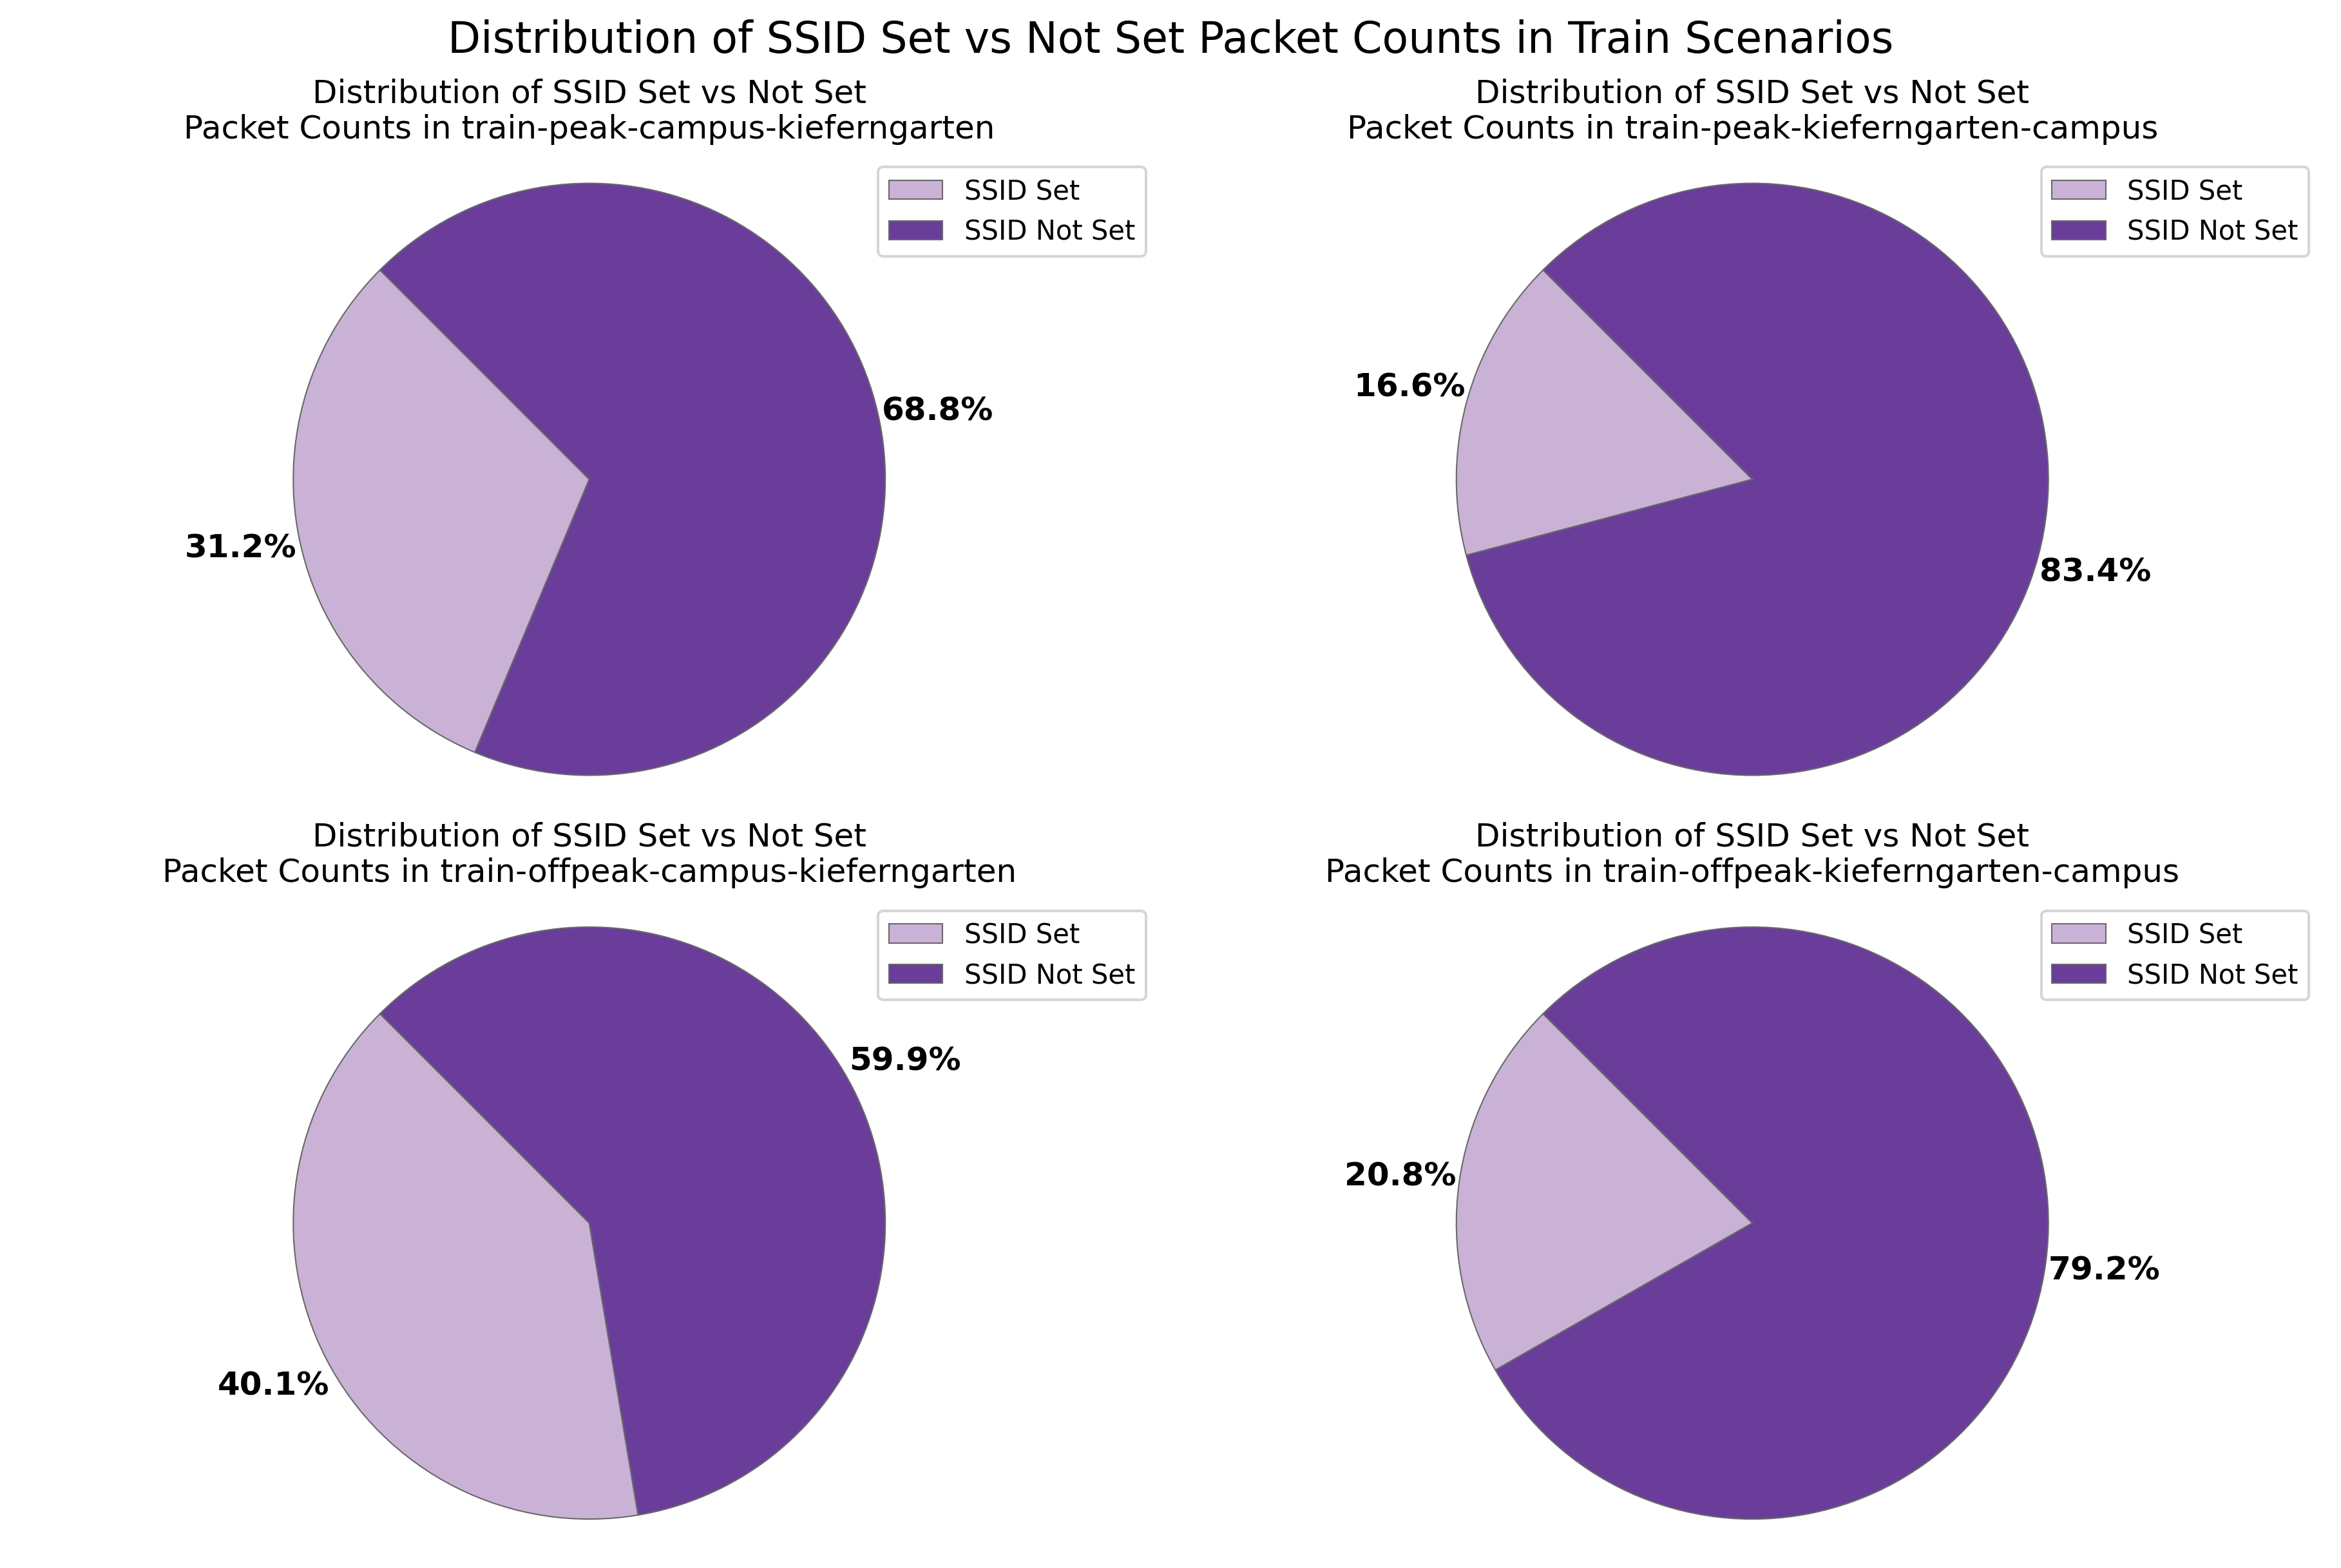
\includegraphics[width=\columnwidth]{images/part1/ssid/train-scenarios.png}
    \caption{SSID Presence in the Train Scenarios}
    \label{fig:ssid_presence_train}
\end{figure}

\begin{figure}
    \centering
    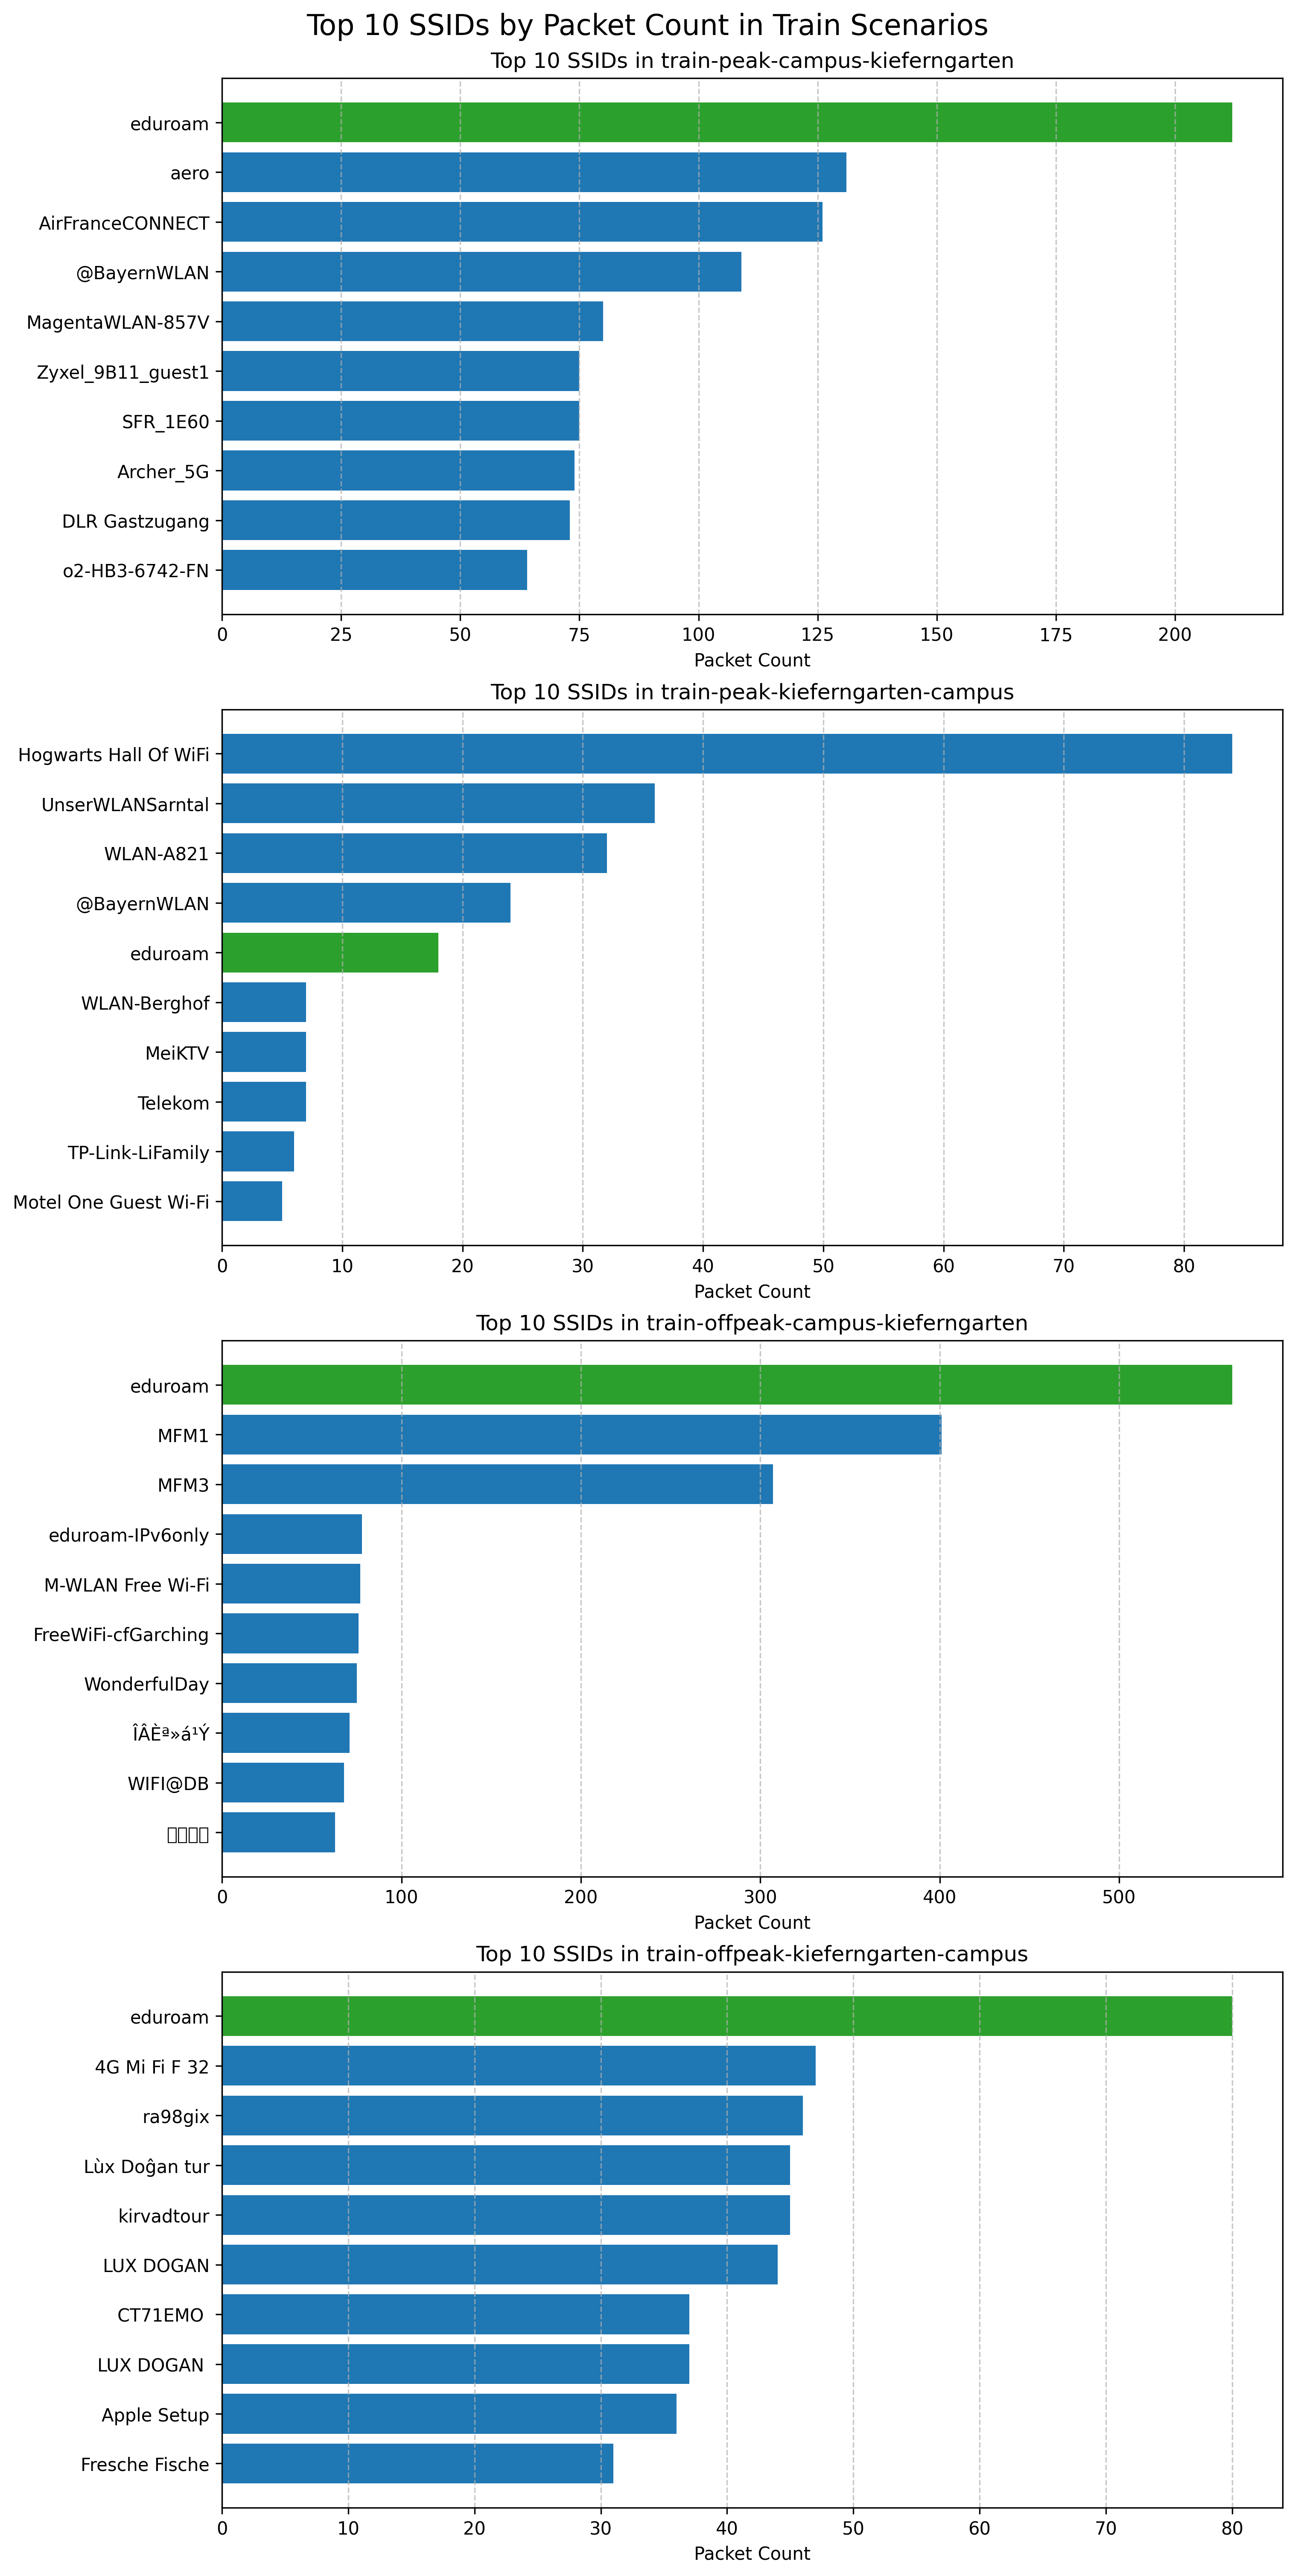
\includegraphics[width=\columnwidth]{images/part1/ssid/top-ssids-train-scenarios.png}
    \caption{Top 10 SSIDs in the Train Scenarios}
    \label{fig:train_ssids}
\end{figure}

Expectedly, just like in the station scenarios, we see that the SSID "eduroam" is the most common in the train scenarios as well, especially in the trains leaving from the Garching Forschungszentrum station.

\subsection{Discussion}
\label{sec:part-1/dis}

Overall, we see that the results of the station and train scenarios are quite different. Although we were able to identify some patterns, we also saw that the results are highly susceptible to a myriad of factors not taken into account, and therefore, it is hard to argue for the correctness of our hypotheses. We strongly argue that the results of this assignment should not be generalized to other environments, and even the patterns argued for should be further investigated with more carefully designed experiments.

Regarding the ethics, we don't collect any information that will tie the MAC addresses to people, nor do we have such information. We also don't disclose the dataset, therefore, like argued in many similar studies (such as the ones we presented in the class), we believe that our approach is ethically sound.

% Interpret the results
% Deeper discussion, speculation on why some results turned out the way they did.

\section{Wi-Fi Traffic Analysis Beyond the MAC Layer}
\label{sec:part-2}

\subsection{Introduction}
\label{sec:part-2/desc}

% Should be short as it is already described in the assignment description/known to the lecturer.
% May even be unnecessary/removed.

% Explain what this section is about
% Explain what we intended to find out
In the second part of this assignment, we turned a Raspberry Pi into a wireless access point, and connected (a) device(s) to it to analyze the flow of packets both in idle and in busy states. The goal was to understand how the distribution of protocols used to communicate changes between different devices and between different scenarios.

\subsection{Setup}
\label{sec:part-2/setup}
We connected a Raspberry Pi Model 3 B to our home network through the Ethernet port over a wired connection, and plugged a dongle to create another network interface to propagate a wireless AP. All traffic going into the Raspberry Pi over the AP interface is then forwarded to the wired interface, to allow it to reach the Internet, as described in the hardware setup. \cref {sec:hardware_setup}.

\subsubsection{Capture setup}
\label{sec:part-2/da-co}
To record all network traffic, we used the \verb|capture.sh| script as described in the capture setup \cref{sec:capture_setup}, with the \verb|-m network| flag which forces the capture of all network traffic on a network interface.

\subsubsection{Hardware Setup}
Additionally, we connected two different clients to the access point: a 2020 Apple iPad 8th generation with iPadOS 18.5 and a 2020 Apple MacBook Air with an M1 chip with MacOS 15.5 (24F74). This setup allows us to compare a tablet with a laptop. One limitation of this configuration is that both devices are from the same vendor (Apple), due to the limited availability of alternative test devices. The iPad and the MacBook were connected to the access point simultaneously, and both operated on battery power during the experiment.

\subsubsection{Scenario description}
\label{section:scenario_description}
The experiment is divided into two parts. In the first part, the iPad and the MacBook remain in an idle or standby state with their displays turned off. To determine whether this state affects the results, a key is pressed on the MacBook’s keyboard after approximately 85 seconds, waking the device and turning on the display for the remainder of the recording without logging in. The total recording duration was 128.36 seconds

The second part of the experiment involves active use of the devices. For this part, only the MacBook is actively used, but the iPad is still connected to the Access point. To simulate a typical search process, we entered the query \textit{"Wie macht das Pferd"} (Engl. \textit{"How does the horse sound"}) into the Safari browser's search bar. Afterward, a horse sound was played, followed by a YouTube video of a \href{https://www.youtube.com/watch?v=xYMh68fCo54}{\color{blue}neighing horse}, which was played for approximately 25 seconds. This was intended to simulate video streaming activity. Finally, messages were sent using both WhatsApp and Element Messenger to represent typical communication behavior. This scenario was recorded for 118.98 seconds. 

Additionally, these recordings are done \textbf{consecutively}. This means the second scenario was recorded after the first scenario.
Due to some difficulties with tracking the time correctly during the recording of both scenarios, the duration doesn't really match between the two scenarios. 
Nevertheless, the results of these two scenarios should still be comparable.

%Those two scenarios are now separated and analyzed in one idle and one active use phase to provide a better possibility to analyze the differences between these two phases later. 

\subsubsection{Recording analysis}
To conduct our analysis, we relied on two different Python libraries for processing the different \textit{.pcap} files. First, Scapy\footnote{https://scapy.net/}, which we used for most of the general packet analysis. Second, Pyshark\footnote{https://pypi.org/project/pyshark/}, the Python wrapper for TShark, proved useful for more detailed inspection, such as identifying the highest layer protocol or examining specific packet contents more thoroughly. For the most analytical operations, Scapy offers enough and is also much faster compared to Pyshark.

\subsubsection{Protocol analysis}
Pyshark is mainly used to identify the highest layer protocol using the \texttt{.highest\_layer}-Attribute. This identifies application protocols (QUIC, TLS, DNS, etc.), but also lower-layer protocols, like ARP and ICMP messages. Additionally, it also contains TCP and DATA frames if no higher-layer protocol was detected.

However, packets marked with \texttt{DATA} as the highest-layer protocol in PyShark typically indicate that no higher-level protocol could be identified by the underlying TShark engine. This could be due to TCP overhead, fragmentation, segmentation, or other data types. 
Therefore, this type of higher-layer protocol hasn't been investigated in detail. \cite{wireshark-protocol-hierarchy}

\subsubsection{Encrypted traffic}
To determine whether packets are encrypted, we decided to base our decision on the highest layer protocol because other methods detected ICMP packets, which are usually unencrypted, as encrypted. Therefore, we decided to classify the following protocols as encrypted packets: QUIC, TLS, SSH, HTTPS, SSL, and FTPS as the highest protocol, which are classified as encrypted; all others are considered unencrypted. Additional restriction, compared to the other analytics: Only packets containing the peer's MAC address are considered


\subsubsection{Transferred Data}
The amount of transferred data is calculated by the sent and received packet sizes in bytes, using the uploading traffic with the MAC address of the MacBook/ iPad as the source address, and the downloading traffic with the MAC address as the destination address. 
The size per packet is calculated by \texttt{len(packet)}, where packet is the parsed version using scapy.



\subsection*{IP Ownership Identification Using \texttt{whois}}
\label{sec:whois}

To determine the organization responsible for a given IP address, the \texttt{whois} command-line utility can be used. This tool queries public databases maintained by Regional Internet Registries (RIRs), such as ARIN, RIPE, or APNIC \footnote{\texttt{man whois}}.

For example, to identify the owner of the IP address \texttt{216.58.206.68}, the following command can be executed in a terminal:

\begin{verbatim}
whois 216.58.206.68
\end{verbatim}

The output will include information such as:

\begin{verbatim}
OrgName:    Google LLC
CIDR:       216.58.192.0/19
NetName:    GOOGLE
\end{verbatim}

The OrgName indicates the organisation to which the IP address belongs. In this case, the answer shows that the IP address belongs in this case to Google.



% Explain the data collection scenarios
% Explain the data collection techniques
%    What is used to collect data
%    How the data is collected/annotated (e.g. timing on the train)
%    Why is it done this way

\subsection{Results}
\label{sec:part-2/ana}
In this section, we evaluate and compare the analytical results of the two scenarios described in \cref{section:scenario_description}.

\subsection{General Details}
\label{sec:part2:general_details}

The recording of the first scenario comprises \textbf{999 packets} transmitted over a duration of \textbf{128.36 seconds}, resulting in an average packet rate of approximately \textbf{7.78 packets per second}. In contrast, the second scenario consists of \textbf{27,510 packets} recorded over \textbf{118.96 seconds}, corresponding to a significantly higher packet rate of approximately \textbf{231.25 packets per second}.

This difference in packet rate indicates a higher level of network activity in the second scenario. As expected, this aligns with the context: scenario 1 captures a baseline or idle state while the devices are located, whereas scenario 2 reflects the active use of a device during video streaming. The elevated packet count and transmission rate in the latter case are consistent with the higher demand for data throughput required by continuous multimedia delivery during the short consumption of the YouTube video.

\subsection{Transferred Data}
\label{sec:transfered_data_analysis}
\begin{table}[ht]
\centering
\resizebox{\columnwidth}{!}{
\begin{tabular}{|l|l|r|r|r|}
\hline
\textbf{Scenario} & \textbf{Device} & \textbf{Upload (bytes)} & \textbf{Download (bytes)} & \textbf{Total (bytes)} \\
\hline
1 & MacBook   & 70,117    & 121,057     & 191,174     \\
1 & iPad  & 48,862    & 57,727      & 106,589     \\
\hline
\multicolumn{2}{|l|}{\textbf{Scenario 1 Total}} & \textbf{118,979} & \textbf{178,784} & \textbf{297,763} \\
\hline
2 & MacBook   & 1,154,530 & 19,563,643  & 20,811,760  \\
2 & iPad  & 49,651    & 43,068      & 92,719      \\
\hline
\multicolumn{2}{|l|}{\textbf{Scenario 2 Total}} & \textbf{1,204,181} & \textbf{19,606,711} & \textbf{20,810,892} \\
\hline
\end{tabular}
}
\caption{Total Traffic Volume by Device and Scenario}
\label{tab:traffic_volume}
\end{table}
Table~\ref{tab:traffic_volume} presents the total upload, download, and combined traffic volume for the MacBook and the iPad in our two scenarios. In \textbf{Scenario~1}, where both devices are in idle, the total traffic was  191\,KB for the MacBook and 107\,KB for the iPad, with a combined total of around 298\,KB. In contrast, \textbf{Scenario~2}, representing active usage of the MacBook and the iPad still in idle, shows an increase in traffic, particularly for the MacBook, which generated over 20.8\,MB of total data, accounting for nearly all of the scenario’s combined 20.8\,MB. The iPad’s traffic remained relatively unchanged between scenarios, because it's in both scenarios in idle mode. Additionally, it has a smaller traffic volume in Scenario 2 as in 1 because the recording time is ten seconds shorter. 


\subsection{Results of Protocol Analysis}
\label{sec:part2_results_protocol_analyse}
This is the total traffic, including from the iPad and the MacBook.

\begin{table}[ht]
\centering
\caption{Number, percentage, and total size of packets per highest layer protocol in scenario one during idle}
\begin{tabular}{lrrr}
\toprule
Protocol & Number of Packets & Percentage & Total Size (Bytes) \\
\midrule
QUIC & 293 & 29.33\% & 163036 \\
TCP & 217 & 21.72\% & 60927 \\
MDNS & 166 & 16.62\% & 60915 \\
TLS & 122 & 12.21\% & 33910 \\
DNS & 64 & 6.41\% & 11273 \\
ARP & 30 & 3.00\% & 3862 \\
ICMPV6 & 30 & 3.00\% & 4229 \\
DATA & 22 & 2.20\% & 5994 \\
IGMP & 20 & 2.00\% & 1698 \\
NBNS & 18 & 1.80\% & 2577 \\
ICMP & 14 & 1.40\% & 4197 \\
DHCP & 3 & 0.30\% & 502 \\
\midrule
Total & 999 & 100.00\% & 353120 \\
\bottomrule
\end{tabular}
\label{tab:packets_per_protocol_idle}
\end{table}
\begin{figure}[htbp]
    \centering
    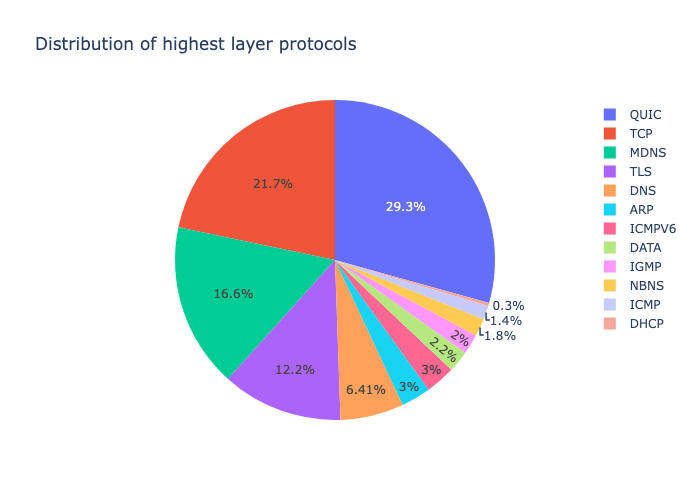
\includegraphics[width=\columnwidth]{images/distributionofhighestlayerprotocols.png}
    \caption{Shows the total highest layer protocol distribution in scenario one during idle}
    \label{fig:protocol_distribution_total_idle}
\end{figure}


\begin{table}[ht]
\centering
\caption{Number, percentage, and total size of packets per highest layer protocol in scenario two during active usage}
\begin{tabular}{lrrr}
\toprule
Protocol & Number of Packets & Percentage & Total Size (Bytes) \\
\midrule
QUIC & 22642 & 82.30\% & 18030492 \\
TCP & 3064 & 11.14\% & 1844451 \\
TLS & 1622 & 5.90\% & 885963 \\
DNS & 132 & 0.48\% & 37707 \\
ARP & 24 & 0.09\% & 5819 \\
ICMPV6 & 13 & 0.05\% & 1002 \\
MDNS & 8 & 0.03\% & 4488 \\
DATA & 3 & 0.01\% & 1694 \\
ICMP & 2 & 0.01\% & 144 \\
\midrule
Total & 27510 & 100.00\% & 20811760 \\
\bottomrule
\end{tabular}
\label{tab:packets_per_protocol_active}
\end{table}


Tables~\ref{tab:packets_per_protocol_idle} and~\ref{tab:packets_per_protocol_active} show that traffic during idle is more evenly distributed across protocols, with QUIC at 29.33\%. In contrast, active usage is dominated by QUIC traffic (82.30\%) and generates significantly higher volume. Local protocols like MDNS and ARP are more prominent during idle, while application-level traffic drives the increase during active use. Additionally, we can see that the management local protocols IGMP (\cref{sec:igmp}), NBNS (\cref{nbns}), and DHCP (\cref{sec:dhcp}) only occur in the first scenario. One reason could be that during scenario one, the devices discover each other, and in the following recording in scenario 2, the discovery of services and the receiving of the IP address are already finished.


 

\subsection{Results of the encrypted traffic}
\label{sec:part2_encrypted_traffic}
\begin{figure}[htbp]
    \centering
    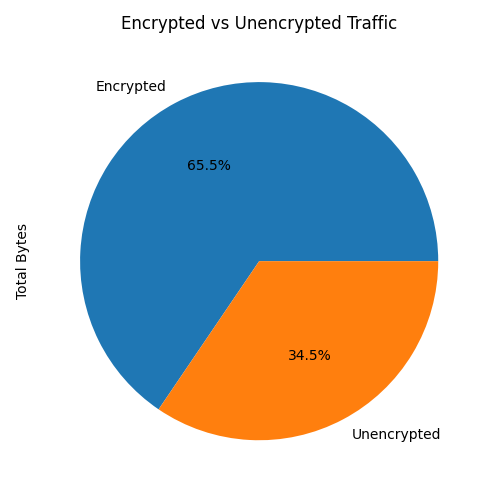
\includegraphics[width=\columnwidth]{images/part2/idle/encrypted_vs_unencrypted.png}
    \caption{Shows the share of the encrypted and unencrypted traffic protocols, when the MacBook is in the locked screen (idle) during scenario 1.}
    \label{fig:encryption_idle}
\end{figure}
\begin{figure}[htbp]
    \centering
    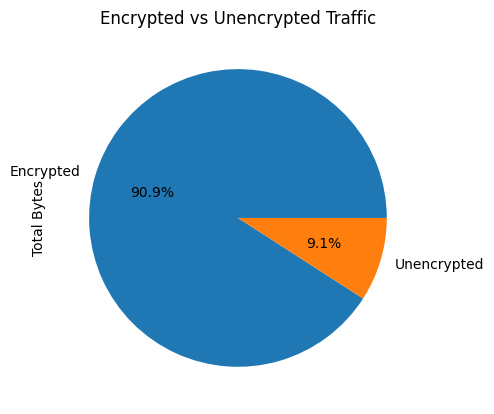
\includegraphics[width=\columnwidth]{images/part2/active use/encrypted_traffic.png}
    \caption{Shows the share of the encrypted and unencrypted traffic protocols, when the MacBook is actively used during scenario 2}
    \label{fig:encryption_active}
\end{figure}
During \textbf{Scenario~1} (\cref{fig:encryption_idle}), approximately two-thirds of the traffic is encrypted, while one-third is unencrypted. In contrast, \textbf{Scenario~2} (\cref{fig:encryption_active}) shows a significantly higher share of encrypted traffic—around 90\%—with only about 10\% unencrypted. This shift is primarily due to the distribution of protocols, discussed in detail in \cref{sec:part2_results_protocol_analyse}. In Scenario~1, unencrypted local management protocols (e.g., MDNS, ARP) contribute noticeably to the traffic. In Scenario~2, high-volume encrypted application protocols such as QUIC dominate, and some local protocols are no longer present.






%To analyse the traffic between the peers and the participating parties, we relied on the IP addresses of the corresponding peers. 
% \begin{figure}[htbp]
%     \centering
%     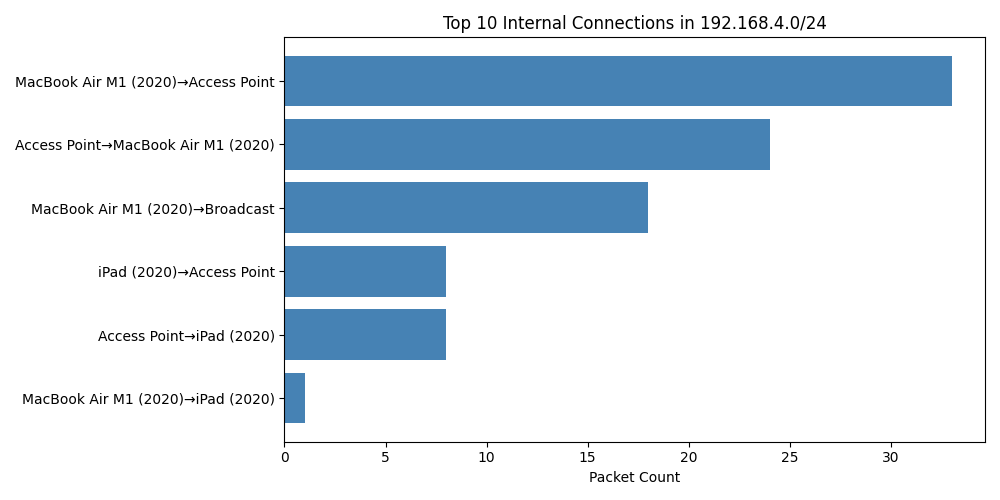
\includegraphics[width=\columnwidth]{images/internal_traffic_top_peers_idle.png}
%     \caption{This shows the number of packets for each direction between the peers during the idle time}
%     \label{fig:top_peers_idle}
% \end{figure}


\begin{figure}[htbp]
    \centering
    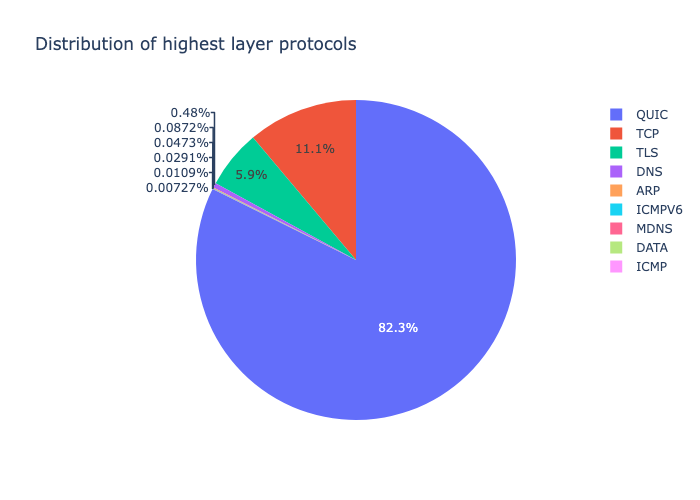
\includegraphics[width=\columnwidth]{images/part2/active use/distributionofhighestlayerprotocols.png}
    \caption{Shows the total highest layer protocol distribution in scenario two during active usage}
    \label{fig:protocol_distribution_total_active}
\end{figure}


\subsubsection{Investigating the arrival time of all protocols}

\begin{figure}[htbp]
    \centering
    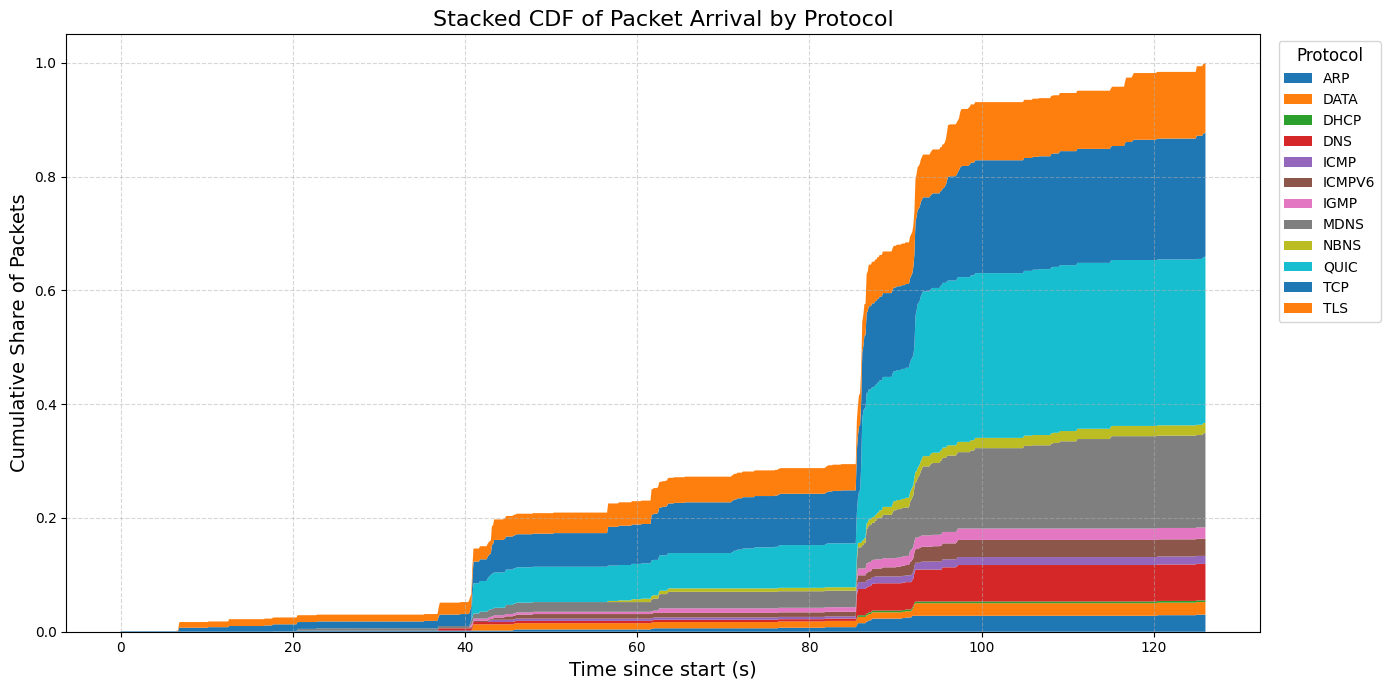
\includegraphics[width=\columnwidth]{images/part2/idle/cdf_idle_all_protocols.png}
    \caption{CDF of the arrival rate of packets per protocol during the first scenario}
    \label{fig:cdf_total_protocols_idle}
\end{figure}

\begin{figure}[htbp]
    \centering
    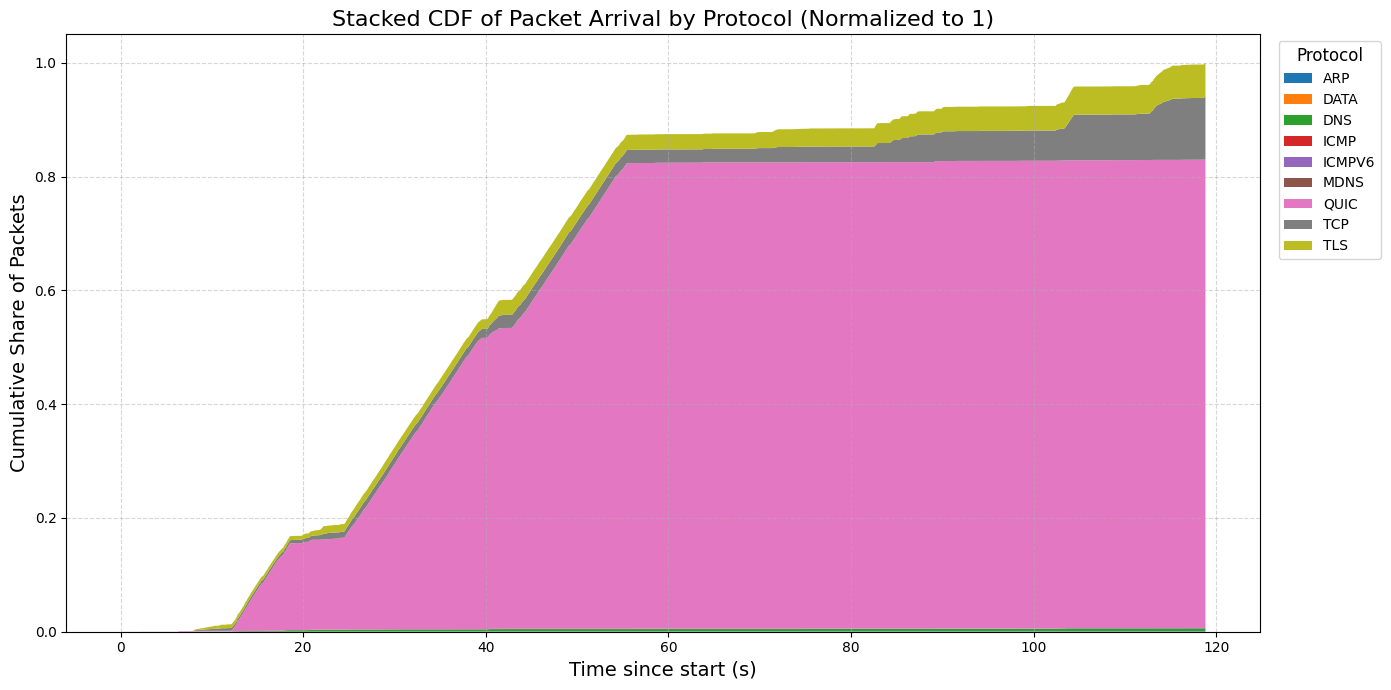
\includegraphics[width=\columnwidth]{images/part2/active use/cdf.png}
    \caption{CDF of the arrival rate of packets per protocol during the second scenario}
    \label{fig:cdf_total_protocols_active}
\end{figure}
% \cref{fig:cdf_total_protocols_idle} and \cref{tab:packets_per_protocol_active} show both the CDF of the packets and are normalized by one.
% Investigating the different plots, we can see different things. 
% \cref{fig:cdf_total_protocols_idle} can be split into 3 different intervals. In the first 40 seconds, only a few packets are sent, which are mostly TLS and TCP packets. After 40 seconds, the number of packets increases by many QUIC and local discovery protocols like mDNS. At around second 85, the display of the Mac is turned on, and the number of packets increases drastically by a high increase of QUIC packets, MDNS, NBNS, and DNS requests. The main reason should be here, that the MacBook becomes active, and the background services try to discover the local network and update itselves.   
% In \cref{tab:packets_per_protocol_active}, which belongs to Scenario 2, the QUIC protocol clearly dominates. 
% It increases after around 10 seconds until circa 55 seconds very rapidly and remains afterward relatively constant. The reason for this could be because during this interval, google.com and youtube.com are opened and loading the first 27 seconds of the video, which are already loaded at the beginning. After this interval, the share of TCP and TLS packets are increasing due to the use of writing a message via whatsapp and element. 
\Cref{fig:cdf_total_protocols_idle} and \cref{tab:packets_per_protocol_active} both show the cumulative distribution function (CDF) of packet arrivals per protocol, normalized to one. These visualizations provide insight into the temporal dynamics and relative contribution of each protocol during Scenario~1 (idle) and Scenario~2 (active use).

In \cref{fig:cdf_total_protocols_idle}, which corresponds to Scenario~1, the packet arrival behavior can be divided into three distinct intervals. In the first 40 seconds, only a small number of packets are exchanged, primarily consisting of low-frequency TLS and TCP traffic, likely background system keep-alives or encrypted status checks. Between seconds 40 and 85, the packet rate increases moderately, and additional protocols such as QUIC and local discovery services like mDNS begin to appear more frequently. Around the second of 85, a sharp rise in packet arrivals occurs. This increase is marked by a burst of QUIC, mDNS, NBNS, and DNS packets. The timing is related with the reactivation of the MacBook display, which likely triggers background services to resume local network discovery and perform updates or synchronizations. This behavior indicates a shift from passive idle traffic to network activity driven by system re-engagement.

\Cref{tab:packets_per_protocol_active}, representing Scenario~2, reveals a very different profile. QUIC traffic dominates the packet flow, comprising the vast majority of early and total transmissions. The QUIC share rises sharply between 10 and 55 seconds, reflecting the loading of external services such as \texttt{google.com} and \texttt{youtube.com}, with video preloading likely accounting for the early peak. After this initial phase, the growth of QUIC stabilizes, while the presence of TCP and TLS increases steadily. This change aligns with messaging activity through apps such as WhatsApp and Element, which rely more heavily on HTTPS-based encrypted communication. Compared to the idle case, the protocol diversity in Scenario~2 is lower, but the volume and rate of transmission are significantly higher and more bursty—characteristic of interactive application usage.

% \begin{figure}[htbp]
%     \centering
%     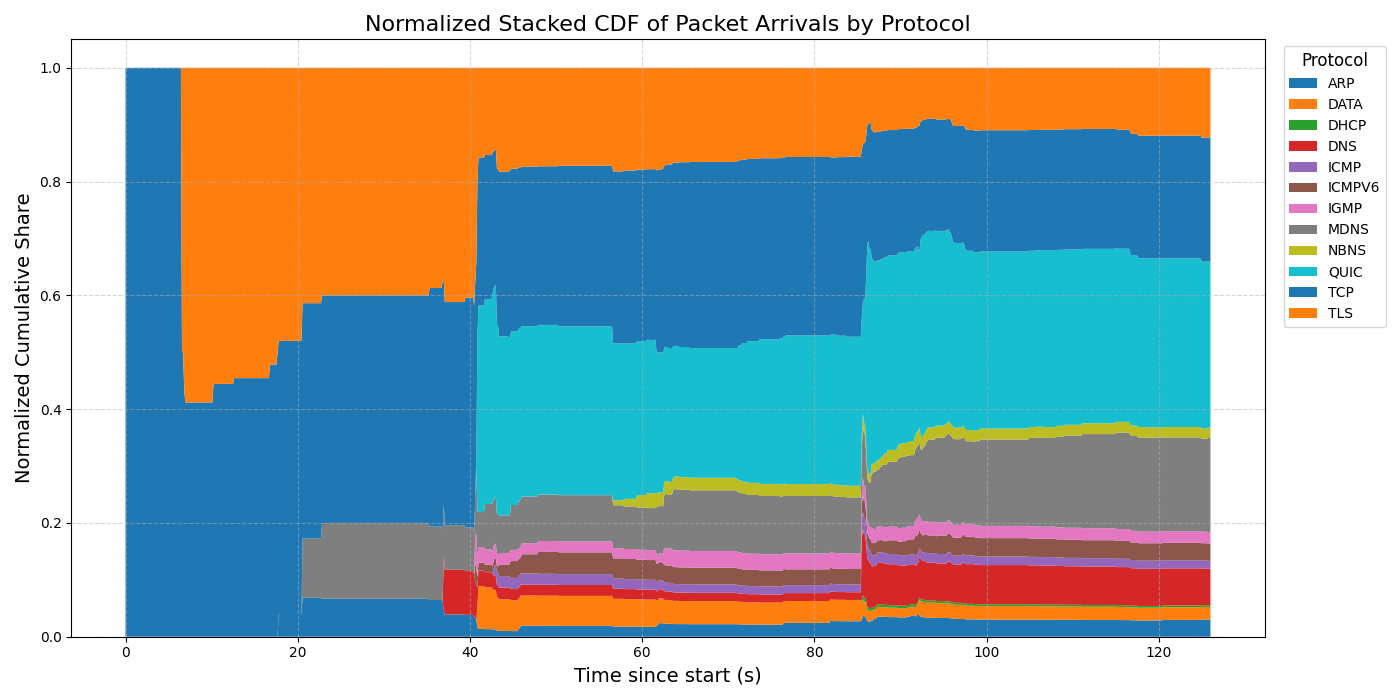
\includegraphics[width=\columnwidth]{images/part2/idle/normalized_stacked_cdf_packet_arrival.png}
%     \caption{The graph shows a CDF of the packet arrival normalized over all values. The result is the total share per protocol for each second for the first scenario.}
%     \label{fig:cdf_total_protocols_idle}
% \end{figure}



% \begin{figure}[htbp]
%     \centering
%     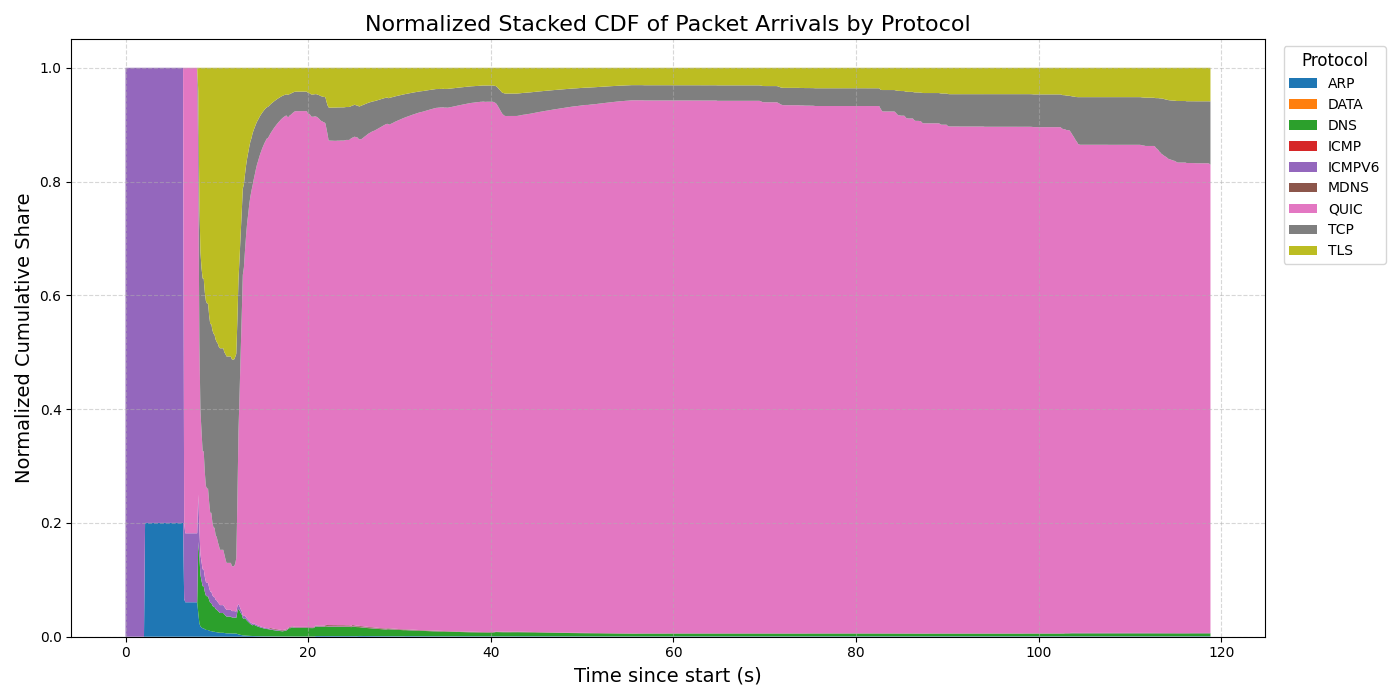
\includegraphics[width=\columnwidth]{images/part2/active use/normalized_stacked_cdf_packet_arrival.png}
%     \caption{The graph shows a CDF of the packet arrival normalized over all values. The result is the total share per protocol for each second for the second scenario.}
%     \label{fig:cdf_total_protocols_active}
% \end{figure}

% \begin{figure}[htbp]
%     \centering
%     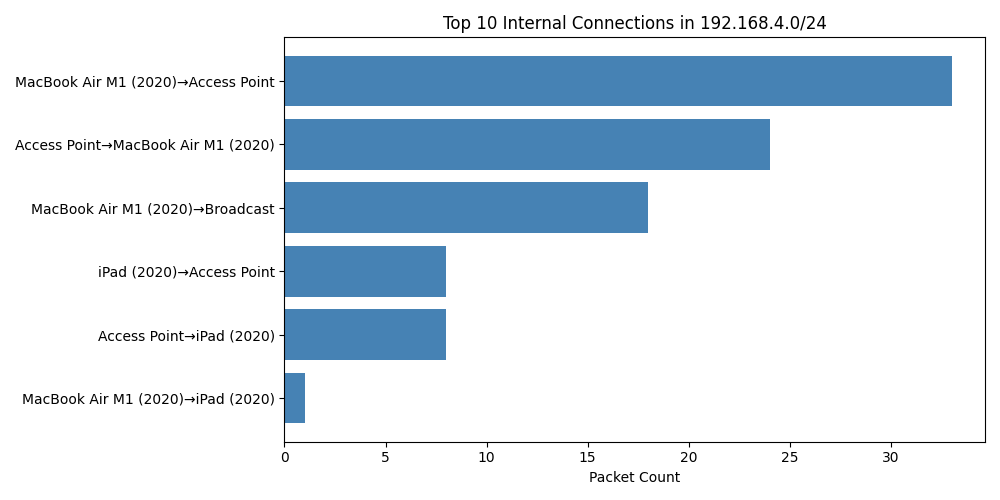
\includegraphics[width=\columnwidth]{images/internal_traffic_top_peers_idle.png}
%     \caption{This shows the number of packets for each direction between the peers during the idle time}
%     \label{fig:top_peers_idle}
% \end{figure}
% What data analysis techniques are used to derive what information
\subsection{Analysis per protocol}

\subsubsection{ARP}
\label{sec:arp}

ARP is a protocol to get the MAC address of the corresponding IPv4 address. 
\begin{figure}[htbp]
    \centering
    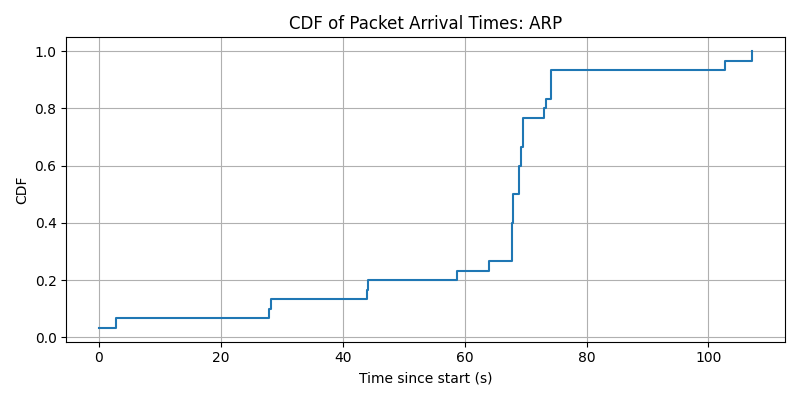
\includegraphics[width=\columnwidth]{images/part2/idle/CDF_ARP.png}
    \caption{CDF of the arrival rate of ARP packets in scenario 1}
    \label{fig:cdf_total_protocols_idle}
\end{figure}

\begin{figure}[htbp]
    \centering
    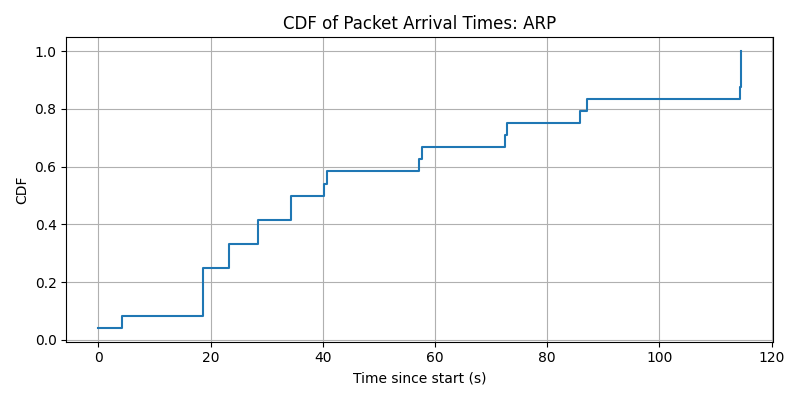
\includegraphics[width=\columnwidth]{images/part2/active use/CDF_ARP.png}
    \caption{CDF of the arrival rate of ARP packets in scenario 2}
    \label{fig:cdf_arp_a}
\end{figure}
In scenario 2 \cref{fig:cdf_arp_a}, the ARP packets appear regularly. 
In contrast to scenario 1, \cref{fig:cdf_arp_a}, where the ARP packets increase mostly, when the display of the Mac is activated.
\subsubsection{IGMP}
\label{sec:igmp}
ICMP (Internet Group Management Protocol) is a protocol where IPv4 hosts can subscribe and unsubscribe to multicast groups, so the router can forward corresponding traffic \cite{rfc2236}.

In scenario one, twenty IGMP packets were captured—ten "Leave Group" messages and ten "V2 Membership Report" messages. The packets were not linked to any specific multicast group. Most were sent from the iPad to two common multicast destinations, each appearing eight times. Less frequent were packets from the MacBook, each destination appearing twice. The traffic relates to Apple's mDNS (Bonjour) protocol, which is discussed in \cref{sec:idle_DNS_mDNS}, where devices dynamically join and leave multicast groups to support service discovery ~\cite{so_multicast_224001251}.



% \begin{figure}[htbp]
%     \centering
%     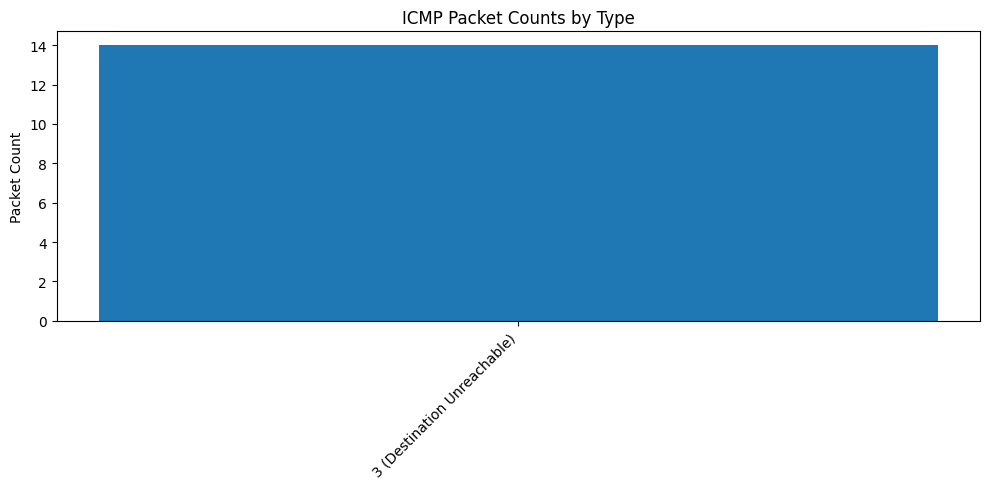
\includegraphics[width=\columnwidth]{images/part2/idle/icmp_local_type_analysis.png}
%     \caption{Number of ICMP packets per type}
%     \label{fig:icmp_idle}
% \end{figure}


\subsubsection{QUIC}
The main reason for the high percentage of QUIC in (\cref{tab:packets_per_protocol_active}) is the traffic to Google by connecting to \texttt{google.com} and \texttt{youtube.com}, and video streams are relatively resource hungry. Google uses QUIC for its processes. To prove that, we looked at the 3 most used IP addresses 173.194.182.201, 142.250.186.110, 216.58.206.68  up (compare \cref{sec:whois}), which are all belonging to Google. 
In Section one(\cref{tab:packets_per_protocol_idle}), most of the QUIC traffic to IP addresses from Apple, like 17.253.56.207, which could be part of the background update service from Apple.


\subsubsection{DHCP}
\label{sec:dhcp}
The DHCP requests only appear at the beginning of section 1 of the recording, where the MacBook requests an IPv4 address from the AP. Afterwards, it already has its IP address and doesn't request it again. 
\subsubsection{ICMPv6}

ICMPv6 is, in this case, mainly used for Neighbor Solicitation between the peers using their link-local addresses. 
Additionally, the AP itself sends a router solicitation to the multicast.



\subsubsection{NBNS}
\label{nbns}
NBNS stands for \textbf{NetBIOS Naming Service} and is a legacy name resolution protocol that runs over UDP port 137, used to map human-readable NetBIOS names (like in our case \textit{MACBOOKAIR}) to IPv4 addresses on local networks. It functions similarly to DNS but in a flat namespace and predates modern systems, operating strictly within IPv4 and local broadcast domains. The protocol is still in use for Windows share protocols like "SAMBA", and the protocol is activated by default in Apple to support communication with legacy devices \cite{apple:102050, wireshark:nbns}. 
In scenario one, multiple NBNS  broadcast messages are sent from the MacBook to the broadcast address 192.168.4.255. These include name release, name registration, and name query messages, mostly related to the name "MACBOOKAIR<00>" and "MSBROWSE". The traffic appears to come from a local device announcing and updating its presence on the local network.











%TODO interpret top 





% \subsubsection{The DNS-protocol}
%  Multicast DNS (mDNS) is a zero-configuration networking protocol that enables hostname-to-IP resolution within small local networks without needing a dedicated DNS server. It sends DNS-like queries over UDP port 353 to a multicast address, allowing devices (e.g., printers, computers, IoT gadgets) to respond directly on a .local domain namespace or the current local subnet. \cite{wikipedia:mdns}
% \begin{figure}[htbp]
%     \centering
%     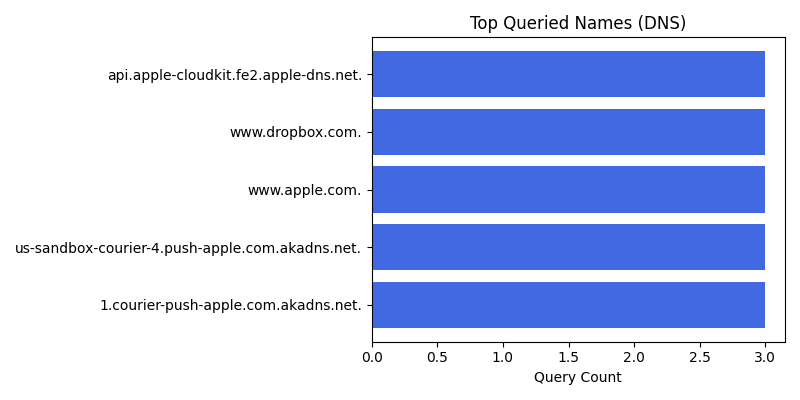
\includegraphics[width=\columnwidth]{images/part2/idle/top_queried_names_dns.png}
%     \caption{Shows the top 5 queried DNS names}
%     \label{fig:dns_names_idle}
% \end{figure}
% When we analyse the DNS requests in \cref{fig:dns_names_idle}, we find that, except for Dropbox, all requested domains are located in the context of Apple. This is since all devices are Apple with the macOS or iOS operating system. In idle mode, these mainly obtain data from Apple in the background. Other Domains have a smaller query count because the devices don't require accessing other services that are responsible for other content. 


% \begin{table*}[ht]
% \caption{Observed domains during idle mode and their functions}
% \label{tab:dns_domains_idle}
% \begin{tabular}{@{}l p{5.5cm}@{}}
% \toprule
% Domain & Function \\
% \midrule
% api.apple-cloudkit.fe2.apple-dns.net. & iCloud API endpoint used to sync app data via CloudKit~\cite{apple_cloudkit}. \\
% www.dropbox.com. & Dropbox file hosting; only non-Apple domain in the capture. \\
% www.apple.com. & Apple homepage; queried by system services for status checks. \\
% us-sandbox-courier-4.push-apple.com.akadns.net. & APNs sandbox endpoint for development/testing notifications~\cite{stackoverflow_apns_sandbox}. \\
% 1.courier-push-apple.com.akadns.net. & APNs production endpoint for background push delivery~\cite{willjessiam}. \\
% \bottomrule
% \end{tabular}
% \end{table*}

% %The first entry \textit{api.apple-cloudkit.fe2.apple-dns.net.} belongs to an iCloud api \cite{apple_cloudkit}. 
% %The third entry \textit{www.apple.com.} is obviously Apple itself. The remaining two entries \textit{1.courier-push-apple.com.akadns.net.} and \textit{us-sandbox-courier-4.push-apple.com.akadns.net.} belong to Apple's push notification API, which is important to receive push-notifications from apps and different services during the idle times. 

% %TODO interpret top 
% \begin{figure}[htbp]
%     \centering
%     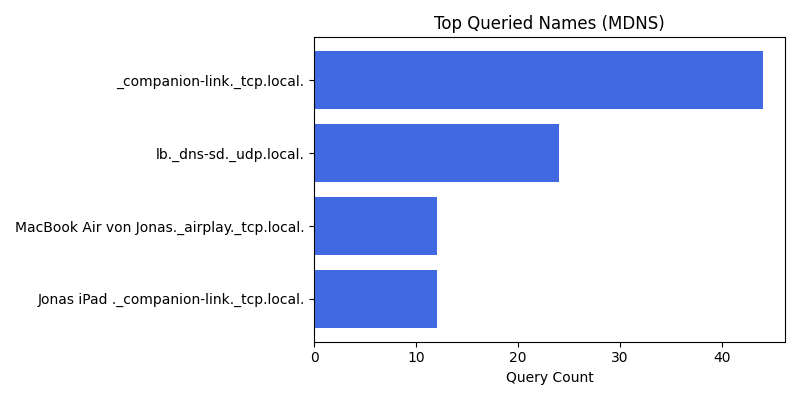
\includegraphics[width=\columnwidth]{images/part2/idle/top_queried_names_mdns.png}
%     \caption{Shows the top 5 queried mDNS names}
%     \label{fig:mdns_idle}
% \end{figure}
% MDNS resolves, in contrast to the DNS requests, only local domains, and the packets are, therefore, directly exchanged between the peers in the local network of the Access Points.
% The top queried Domains, which are shown in \cref{fig:mdns_idle}, belong to Apple's Bonjour protocol to auto discover devices like printers or other Apple devices and determine automatically their IP addresses. Apple devices automatically announce their presence to advertise pairing/linking services. Each device can answer on its own to the requests. For naming each service and device ends on \textit{.local}. By sending out requests for specific services that are device-provided, the querying device can browse through the local network and discover the locally available services of each protocol
% \cite{apple_netservices_introduction}.  
% Regarding the queried domains:
% %todo make it clearer and look on it again
% \begin{itemize}
%     \item \texttt{\_companion-link.\_tcp.local.} belongs to an undocumented TCP service from Apple, but devices are identifiable by it \cite{macpaw_apple_local_network} 
%     \item \texttt{\_dns-sd.\_udp.local.} is a standard mDNS name used in DNS-SD to enumerate all service types on the local network, such as \texttt{\_http.\_tcp.local.}~\cite{cheshire2005dns}
%     \item \texttt{MacBook\ Air\ von\ Jonas.\_airplay.\_tcp.local.} indicates a query for the  local AirPlay service by the iPad to get more information about the availability of the AirPlay service and its IP address~\cite{cheshire2005dns}.
%     \item \texttt{Jonas\ iPad.\_companion-link.\_tcp.local.} indicates an attempt to resolve the MacBook's companion service via Bonjour~\cite{macpaw_apple_local_network}.
% \end{itemize}

% \begin{figure}[htbp]
%     \centering
%     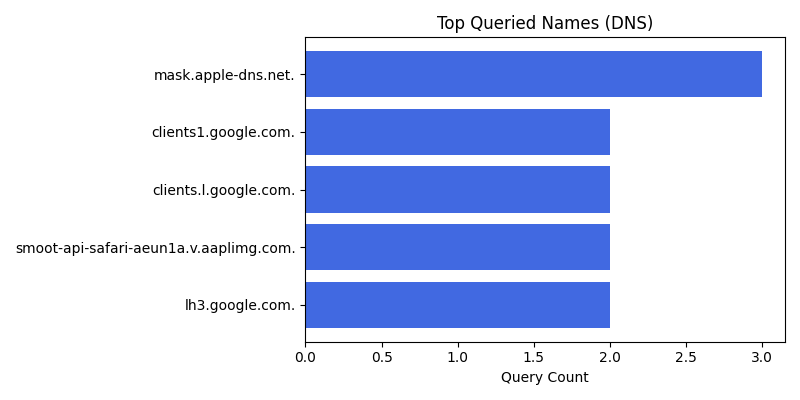
\includegraphics[width=\columnwidth]{images/part2/active use/top_queried_names_dns.png}
%     \caption{Shows the top 5 queried DNS names in active use}
%     \label{fig:dns_active}
% \end{figure}

% \begin{table*}[ht]
% \centering
% \caption{Domains observed in active state and their associated functions}
% \label{tab:idle_dns_domains}
% \begin{tabular}{@{}ll@{}}
% \toprule
% \textbf{Domain} & \textbf{Function} \\
% \midrule
% mask.apple-dns.net. & Used by Apple's iCloud Private Relay to mask DNS queries and IP addresses for user privacy. This comes through the usage of Safari~\cite{apple_mask_dns}. \\
% clients1.google.com. & Endpoint for Google client services, in our case, YouTube and Google search ~\cite{clients1_google_gitlab}. \\
% clients.l.google.com. & Load-balanced alias pointing to Google service endpoints for Google search or YouTube ~\cite{clients_l_google_gitlab}. \\
% smoot-api-safari-aeun1a.v.aaplimg.com. & Apple Safari and Spotlight API endpoint used for suggestions and content lookups~\cite{smoot_api_safari_hn}. \\
% lh3.google.com. & Google image hosting domain for serving photos and thumbnails from Google Photos or Drive~\cite{lh3_google_photos}. \\
% \bottomrule
% \end{tabular}
% \end{table*}

% By comparing the different DNS requests, we can see that during the idle phase (\cref{fig:dns_names_idle}), mostly only domains from Apple are requested, and in the active use phase (\cref{fig:dns_active} the domains from Apple disappear and other Domains are queried through DNS.

% \subsubsection{mDNS}

% \begin{figure}[htbp]
%     \centering
%     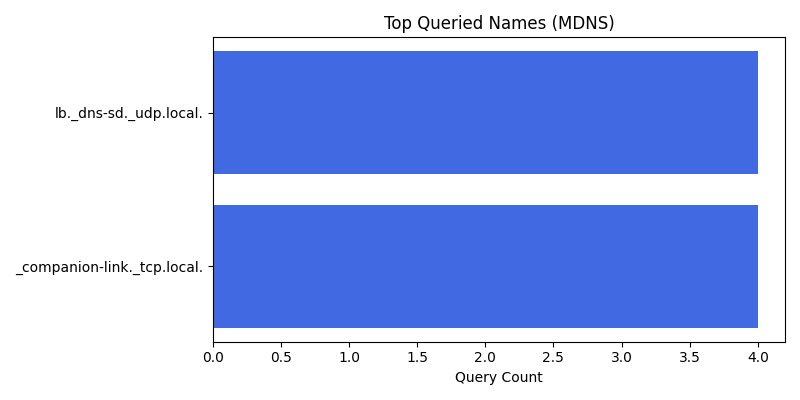
\includegraphics[width=\columnwidth]{images/part2/active use/top_queried_names_mdns.png}
%     \caption{Shows the top 5 queried mDNS names in active use}
%     \label{fig:mdns_active}
% \end{figure}


% Regarding the requested domains in \cref{fig:mdns_active}:
% %todo make it clearer and look on it again
% \begin{itemize}
%     \item \texttt{\_companion-link.\_tcp.local.} belongs to an undocumented TCP service from Apple, but devices are identifiable by it \cite{macpaw_apple_local_network} 
%     \item \texttt{\_dns-sd.\_udp.local.} is a standard mDNS name used in DNS-SD to enumerate all service types on the local network, such as \texttt{\_http.\_tcp.local.}~\cite{cheshire2005dns}
% \end{itemize}

% By comparing the traffic between the active used mDNS (\cref{fig:mdns_active} and during the standby \cref{fig:mdns_idle}, we can observe the reduced number of requests during the active scenario. Additionally, the requests and discovery between the iPad and the MacBook disappeared. The main reason for this could be in \cref{section:scenario_description}, the fact that both scenarios are recorded consecutively. In the first scenario, the devices are trying to discover each other. In the second scenario, the devices have already discovered each other and query the services to see if they are still available.
\subsubsection{DNS and mDNS}
\label{sec:dns_mdns_combined}

Multicast DNS (mDNS) is a zero-configuration networking protocol that enables hostname-to-IP resolution within small local networks without needing a dedicated DNS server. It sends DNS-like queries over UDP port 5353 to a multicast address, allowing devices (e.g., printers, computers) to respond directly on a \texttt{.local} domain namespace or the current subnet \cite{wikipedia:mdns}. It is used, for example, by Apple’s Bonjour protocol for automatic service discovery.

\paragraph{Idle Scenario.}

\begin{figure}[htbp]
    \centering
    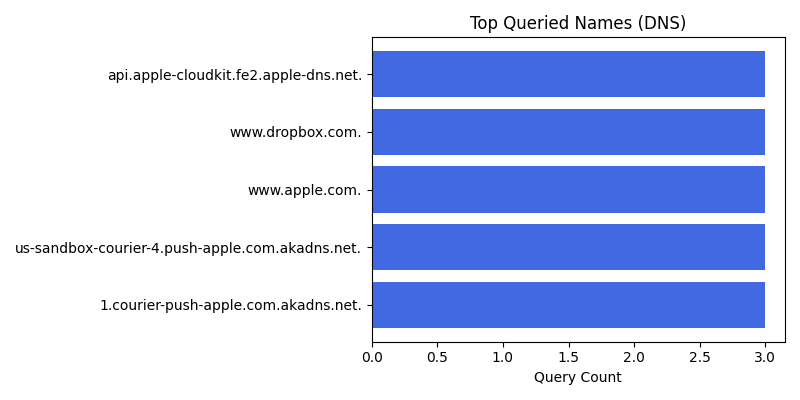
\includegraphics[width=\columnwidth]{images/part2/idle/top_queried_names_dns.png}
    \caption{Top 5 queried DNS names during idle mode}
    \label{fig:dns_names_idle}
\end{figure}

When we analyze the DNS requests in \cref{fig:dns_names_idle}, we find that—except for Dropbox—all requested domains are related to Apple. This is expected, as all devices in the scenario are either macOS or iOS-based. In idle mode, these devices mainly perform background communication with Apple’s services. Other domains have a lower query count because the devices are not actively accessing third-party services.

\begin{table*}[ht]
\caption{Observed domains during idle mode and their functions}
\label{tab:dns_domains_idle}
\begin{tabular}{@{}l p{5.5cm}@{}}
\toprule
Domain & Function \\
\midrule
api.apple-cloudkit.fe2.apple-dns.net. & iCloud API endpoint used to sync app data via CloudKit~\cite{apple_cloudkit}. \\
www.dropbox.com. & Dropbox file hosting; only non-Apple domain in the capture. \\
www.apple.com. & Apple homepage; queried by system services for status checks. \\
us-sandbox-courier-4.push-apple.com.akadns.net. & APNs sandbox endpoint for development/testing notifications~\cite{stackoverflow_apns_sandbox}. \\
1.courier-push-apple.com.akadns.net. & APNs production endpoint for background push delivery~\cite{willjessiam}. \\
\bottomrule
\end{tabular}
\end{table*}

\begin{figure}[htbp]
    \centering
    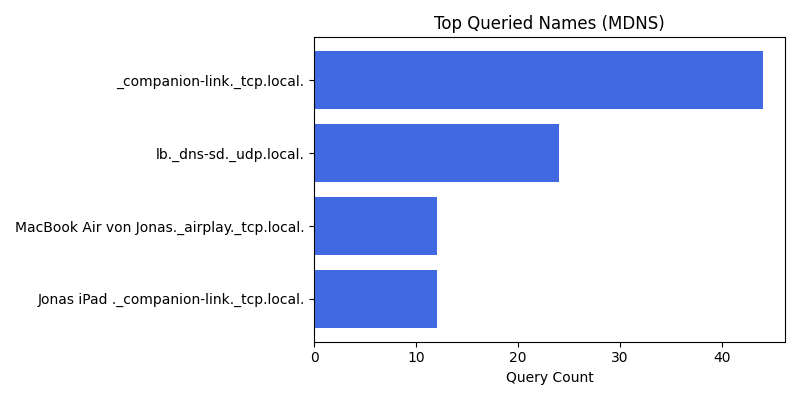
\includegraphics[width=\columnwidth]{images/part2/idle/top_queried_names_mdns.png}
    \caption{Top 5 queried mDNS names during idle mode}
    \label{fig:mdns_idle}
\end{figure}

mDNS, in contrast to DNS, resolves only local domains, and the packets are directly exchanged between peers within the local network. The top queried domains shown in \cref{fig:mdns_idle} mostly belong to Apple’s Bonjour protocol. This is used to automatically discover services like printers or other Apple devices and determine their IP addresses. Devices announce their presence and send out requests for specific services, allowing them to browse locally available protocols.

Regarding the queried domains:

\begin{itemize}
    \item \texttt{\_companion-link.\_tcp.local.} belongs to an undocumented Apple service but is used for identifying devices \cite{macpaw_apple_local_network}. 
    \item \texttt{\_dns-sd.\_udp.local.} is used in DNS-SD to enumerate all service types in the local network, such as \texttt{\_http.\_tcp.local.}~\cite{cheshire2005dns}.
    \item \texttt{MacBook\ Air\ von\ Jonas.\_airplay.\_tcp.local.} is a query sent by the iPad to get availability and IP information of the local AirPlay service~\cite{cheshire2005dns}.
    \item \texttt{Jonas\ iPad.\_companion-link.\_tcp.local.} indicates an attempt to resolve the iPad’s companion service via Bonjour~\cite{macpaw_apple_local_network}.
\end{itemize}

\paragraph{Active Use Scenario.}

\begin{figure}[htbp]
    \centering
    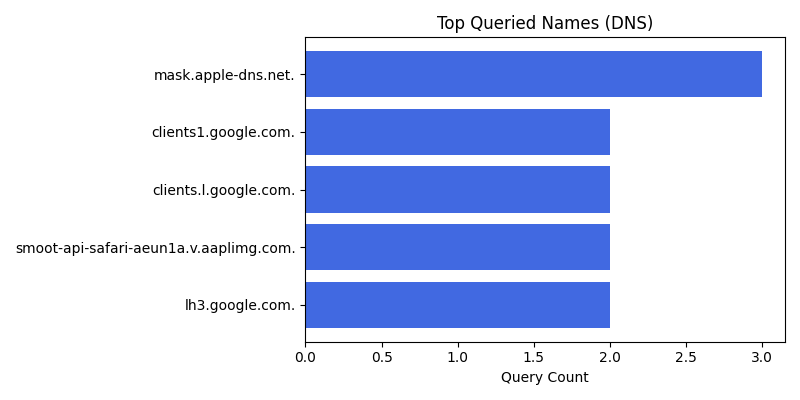
\includegraphics[width=\columnwidth]{images/part2/active use/top_queried_names_dns.png}
    \caption{Top 5 queried DNS names during active use}
    \label{fig:dns_active}
\end{figure}

In contrast, during the active use scenario, the DNS queries change significantly. As seen in \cref{fig:dns_active}, the previously observed Apple domains largely disappear. Instead, services from Google and other third parties become dominant. This is expected, as the device is actively being used to stream a video via YouTube and browse using Safari.

\begin{table*}[ht]
\centering
\caption{Observed domains during active use and their functions}
\label{tab:idle_dns_domains}
\begin{tabular}{@{}ll@{}}
\toprule
\textbf{Domain} & \textbf{Function} \\
\midrule
mask.apple-dns.net. & Used by Apple's iCloud Private Relay to mask DNS queries and IP addresses~\cite{apple_mask_dns}. \\
clients1.google.com. & Endpoint for Google client services, in this case, YouTube and Google search ~\cite{clients1_google_gitlab}. \\
clients.l.google.com. & Load-balanced alias pointing to Google service endpoints ~\cite{clients_l_google_gitlab}. \\
smoot-api-safari-aeun1a.v.aaplimg.com. & Safari and Spotlight API endpoint used for suggestions and content lookups~\cite{smoot_api_safari_hn}. \\
lh3.google.com. & Google image hosting domain (e.g., thumbnails from Google Photos)~\cite{lh3_google_photos}. \\
\bottomrule
\end{tabular}
\end{table*}

\begin{figure}[htbp]
    \centering
    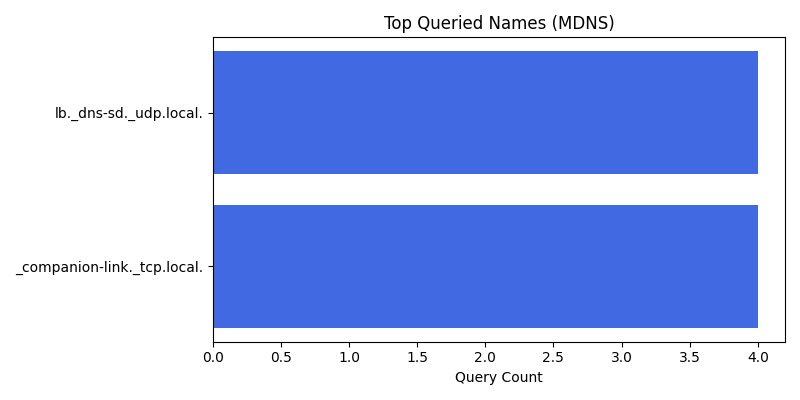
\includegraphics[width=\columnwidth]{images/part2/active use/top_queried_names_mdns.png}
    \caption{Top 5 queried mDNS names during active use}
    \label{fig:mdns_active}
\end{figure}

Looking at the mDNS requests during active use in \cref{fig:mdns_active}, we observe fewer requests overall. The earlier discovery of traffic between the iPad and MacBook (seen in the idle scenario) has disappeared. This is likely due to the fact that the devices have already discovered each other during the idle period. In the active phase, they simply check the availability of previously discovered services.

Relevant domain examples in the active mDNS capture:

\begin{itemize}
    \item \texttt{\_companion-link.\_tcp.local.} — same as before, used for ongoing identification or verification.
    \item \texttt{\_dns-sd.\_udp.local.} — same as before, used for ongoing identification or verification.
\end{itemize}

\paragraph{Comparison.}

By comparing DNS traffic across both scenarios, we see that:

\begin{itemize}
    \item In idle mode (\cref{fig:dns_names_idle}), DNS requests are dominated by Apple services (background updates, iCloud, push notifications).
    \item In active use (\cref{fig:dns_active}), DNS activity reflects actual user interaction: requests to Google, CDNs, and media content providers.
\end{itemize}

The mDNS behavior shows the opposite pattern:

\begin{itemize}
    \item In idle mode (\cref{fig:mdns_idle}), there is a higher number of discovery requests, including device-specific queries.
    \item In active use (\cref{fig:mdns_active}), fewer discovery queries are needed, likely because the devices have already discovered one another and no longer need to repeat the same queries.
\end{itemize}

This behavior aligns with the purpose of each protocol: DNS handles external lookups to Internet domains, while mDNS focuses on local service discovery. The traffic patterns support this distinction and provide insight into how modern Apple devices manage both background and user-driven network activity.


\subsection{Discussion}
To conclude this section and experiment, we investigated the difference in device usage in the network trace of these devices. In order to compare whether the observation also applies to different types of devices from different manufacturers, further investigations would have to be carried out. Unfortunately, since only Apple devices were available, it was only possible to compare them with each other. Additionally, the analysis is limited by the protocol-wise analysis by assuming the iPad and the MacBook are one device and are analyzed together. To get a more comprehensive view. The devices have to be observed and analysed separately from each other. 

\section*{Acknowledgements}
We acknowledge that GitHub Copilot was utilized to help with writing the code for refining plots, and Grammarly was utilized to correct typos and punctuation mistakes. 
%todo investigate more 

%\subsection{Results}
%\label{sec:part-2/res}

% Should be only descriptive
%    No need to interpret
% Plots, numbers, etc.

%\subsection{Discussion}
%\label{sec:part-2/dis}

% Interpret the results
% Deeper discussion, speculation on why some results turned out the way they did.

%%
%% The next two lines define the bibliography style to be used, and
%% the bibliography file.
\bibliographystyle{ACM-Reference-Format}
\bibliography{references}

\end{document}
\endinput
%%
%% End of file `sample-sigconf-authordraft.tex'.
